\chapter{Expérimentations}


\renewcommand{\leftmark}{EXPERIMENTATIONS}

\section{Matériel}

\subsection{Radio logicielle}

La radio logicielle \textit{(Software Defined Radio, SDR)} est une technologie qui permet de mettre en œuvre des systèmes de radio à l'aide de logiciels plutôt que de matériels. Le site RTL-SDR \footnote{RTL-SDR : \href{https://www.rtl-sdr.com/about-rtl-sdr/}{https://www.rtl-sdr.com/about-rtl-sdr/}} donne des informations sur le fonctionnement des radios logicielles, et mentionne également les SDRs utilisées pour ce travail.

\vspace{0.1cm}

Dans les systèmes de radio traditionnel, les différentes fonctions de la radio, comme l'accord sur une fréquence spécifique, la modulation et la démodulation du signal, et le filtrage du bruit, sont mis en œuvre à l'aide de composants matériels tels que des oscillateurs, des amplificateurs et des filtres. En revanche, les systèmes SDR utilisent des logiciels pour effectuer ces fonctions, ce qui les rend beaucoup plus flexible car chaque composante est reconfigurable. Les radios logicielles sont capables d'opérer sur une large portée de fréquences, aussi bien très basse fréquence que haute fréquence.
Les SDR peuvent jouer le rôle d'émetteur ou de récepteur ou les deux. Différentes radios logicielles sont testées pour ce travail, ce qui est motivé pour plusieurs raisons. Tout d'abord cela permet d'observer certaines variations (comme la qualité du signal, la distance) entre les différents récepteurs pour une même expérience et ainsi définir la SDR la plus adéquate. Ensuite, la diversité de radios logicielles permet d'approfondir l'apprentissage de cette technologie et de comprendre plus aisément le fonctionnement d'une radio logicielle. Une version plus simple permet d'assimiler les bases de la pratique avec une SDR, mais pouvoir utiliser des versions plus abouties permet d'expérimenter de manière plus précise les expériences.

\newpage

\subsubsection{RTL SDR DVB-T}\label{dvbt}

La \textit{RTL SDR DVB-T} est la version la moins chère des radios utilisées. Cette radio est initialemnt utilisée pour recevoir des signaux DVB-T (\textit{Digital video broadcasting Terrestrial} télévisés. La figure \ref{term31} montre la radio, qui est un device USB qui inclu un \textit{chipset RTL2832U} et un \textit{RF tuner chip}.

\begin{figure}[h]
\centering

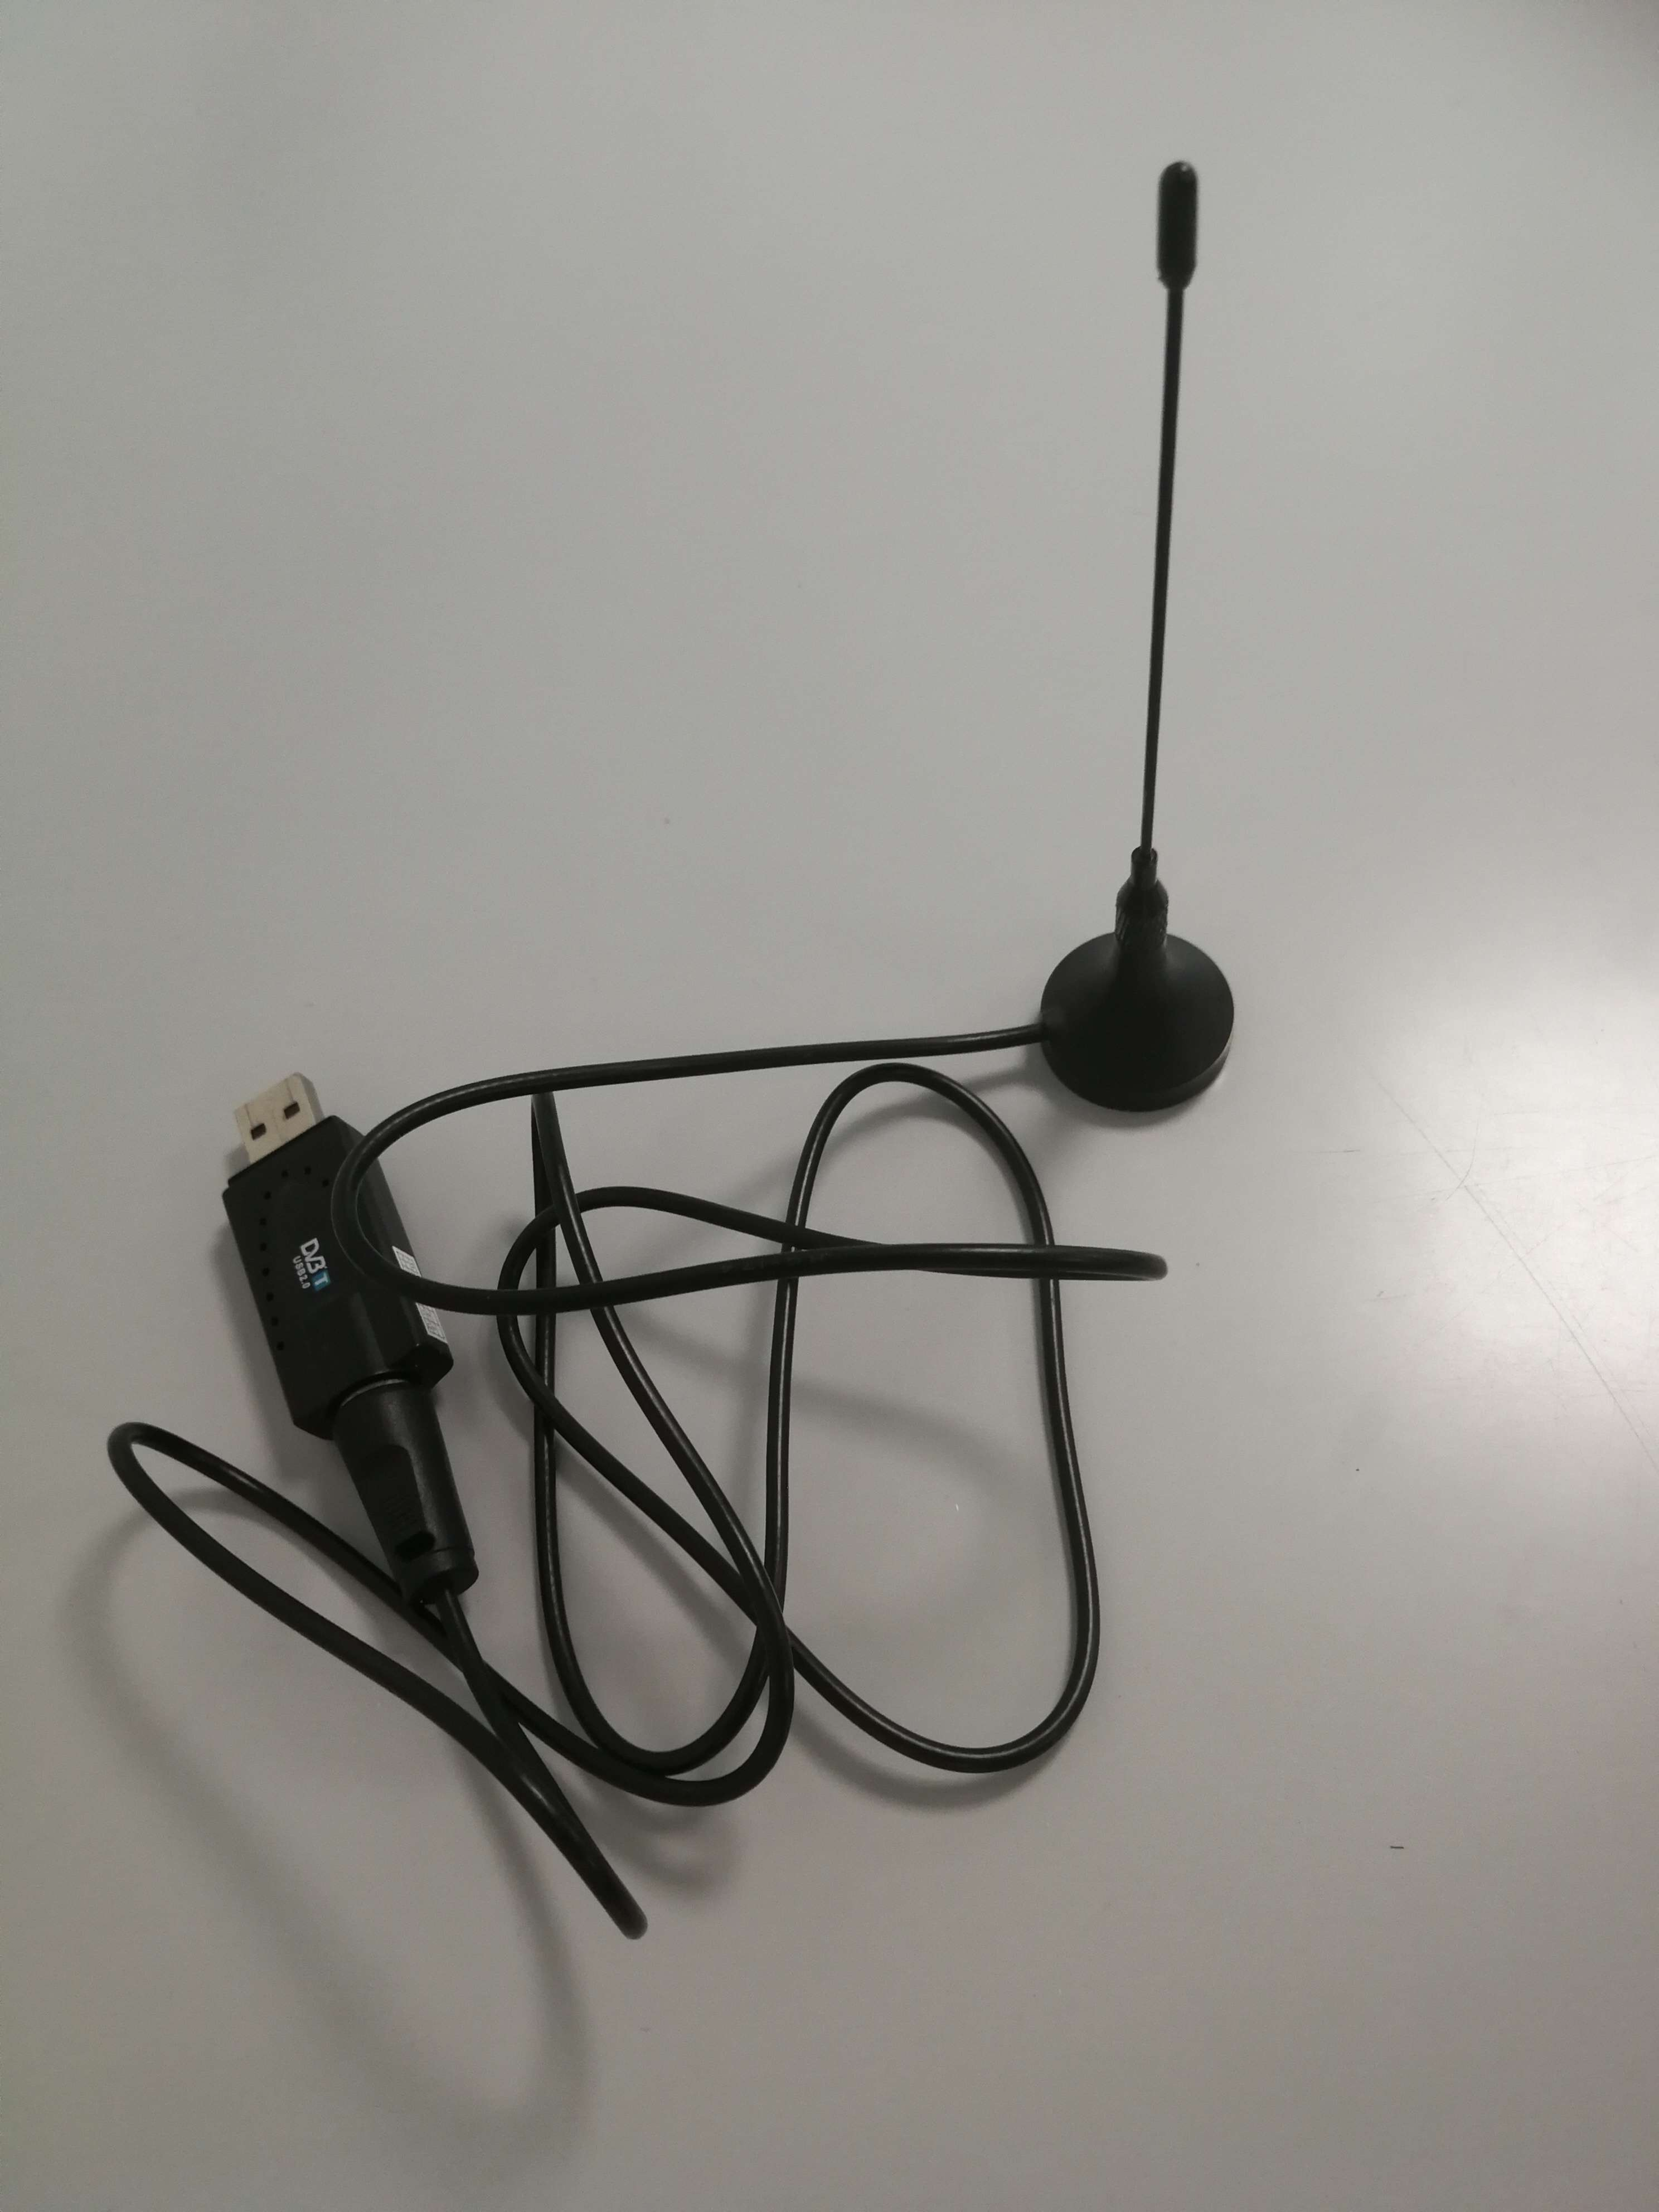
\includegraphics[scale=0.08]{images/dvbt.png}
\caption{RTL SDR DVB-T dongle}\label{term31}
\end{figure}

Le chipset RTL2832U digitalise les signaux RF et les envoie à l'ordinateur. Le tuner permet d'ajuster la fréquence pour couvrir une large portée.
La radio est raccordée à l'ordinateur via le port USB. Le site RTL SDR \footnote{RTL-SDR : \href{https://www.rtl-sdr.com/about-rtl-sdr/}{https://www.rtl-sdr.com/about-rtl-sdr/}} ajoute quelques informations sur l'origine de l'utilisation de DVB-T tuner en tant que SDR. Le schéma bloc de la sdr est représenté sur la figure \ref{term3000}. 

\newpage

\begin{figure}[h]
\centering

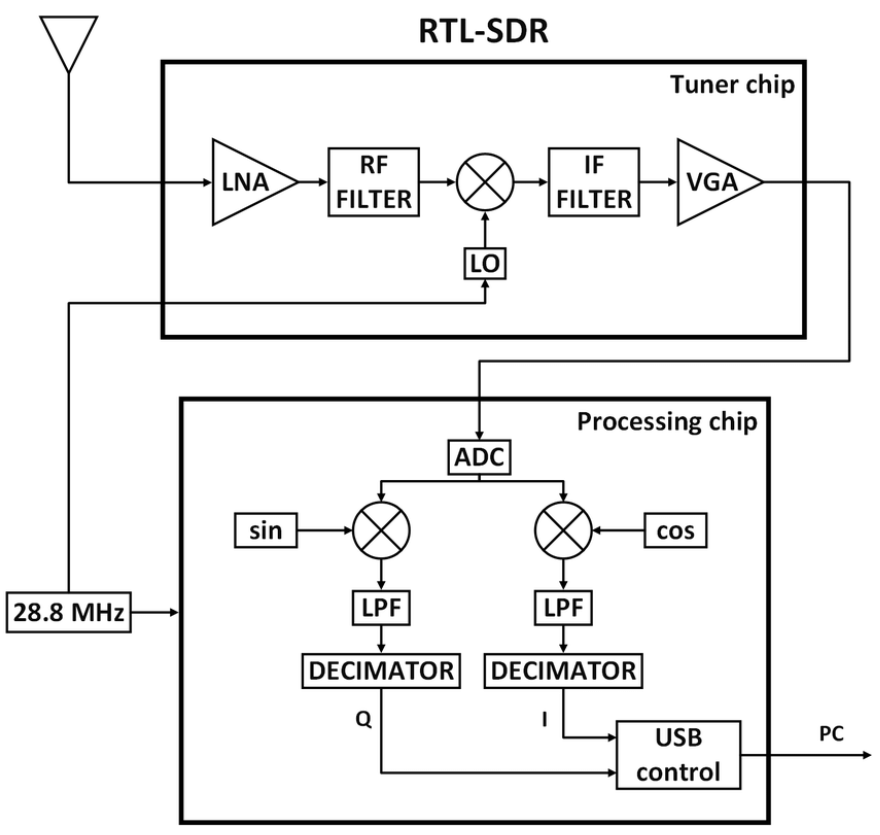
\includegraphics[scale=0.5]{images/SB-rtlsdr.png}
\caption{Schéma bloc de la RTL SDR\cite{SBrtlsdr}}\label{term3000}
\end{figure}


Le tuner comporte les différentes éléments :
\begin{itemize}
\item \textbf{Low Noise Amplifier (LNA)}. le LNA amplifie le signal tout en minimisant l'ajout de bruit, afin de maintenir un SNR faible.
\item \textbf{Radio Frequency Filter (RF Filter)}. Le filtre permettant d'isoler la fréquence désirée.
\item \textbf{Local oscillator (LO)}. La fréquence de l'oscillateur local n'est pas fixe, mais elle est contrôlée par un circuit PLL qui utilise une horloge de référence de 28,8 MHz. Cela permet à la SDR d'opérer sur une plage de fréquence approximative entre 24 MHz et 1,7 GHz. L'utilisation de l'oscillateur local, réglable par le PLL, couplée au signal reçu, produit un signal à une fréquence intermédiaire..
\item \textbf{Itermediate Frequency Filter (IF Filter)}. Ce filtre permet d'isoler le signal à fréquence intermédiaire. L'utilisation d'une fréquence intermédiaire est importante pour pouvoir opérer sur le signal. Par exemple la démodulation est bien plus abordable sur un signal possèdant une fréquence réduite que sa valeur originale.
\item \textbf{Variable Gain Amplifier (VGA)}. Le VGA ajuste l'amplitude du signal pour maintenir un niveau constant.
\end{itemize}

\vspace{0.1cm}

Le chipset contient les éléments suivants :
\begin{itemize}
\item \textbf{Analog to Digital Converter (ADC)} Le signal sortant du tuner est échantillonné par l'ADC à une fréquence d'échantillonnage de 28.8MHz. L'ADC permet de convertir un signal analogique en signal numérique.
\item \textbf{Digital Down Converter (DDC)} Le signal est ramené en bande de base grâce au DDC. Le Digital Down Converter  mixe le signal avec une sinusoide complexe et ensuite applique un filtre \textbf{Low Pass Filter (LPF)}. 
\item \textbf{Decimator} La dernière étape utilise la décimation pour réduire le taux d'échantillonage du signal.
\item \textbf{USB control} Le signal est réduit uniquement aux échantillons complexes I et Q. Ils sont récupérés depuis l'USB de la SDR.
\end{itemize}

\vspace{0.1cm}

Une description détaillée du déroulement de la récupération du signal par la SDR est disponible sur le site \textit{Ajoo's blog}\footnote{Ajoo's blog : \href{https://ajoo-github-blog-old.pages.dev/intro-to-rtl-sdr-part-i-principles-and-hardware}{https://ajoo-github-blog-old.pages
.dev/intro-to-rtl-sdr-part-i-principles-and-hardware}}.




\subsubsection{RTL-SDR R820T2}

\begin{figure}[h]
\centering

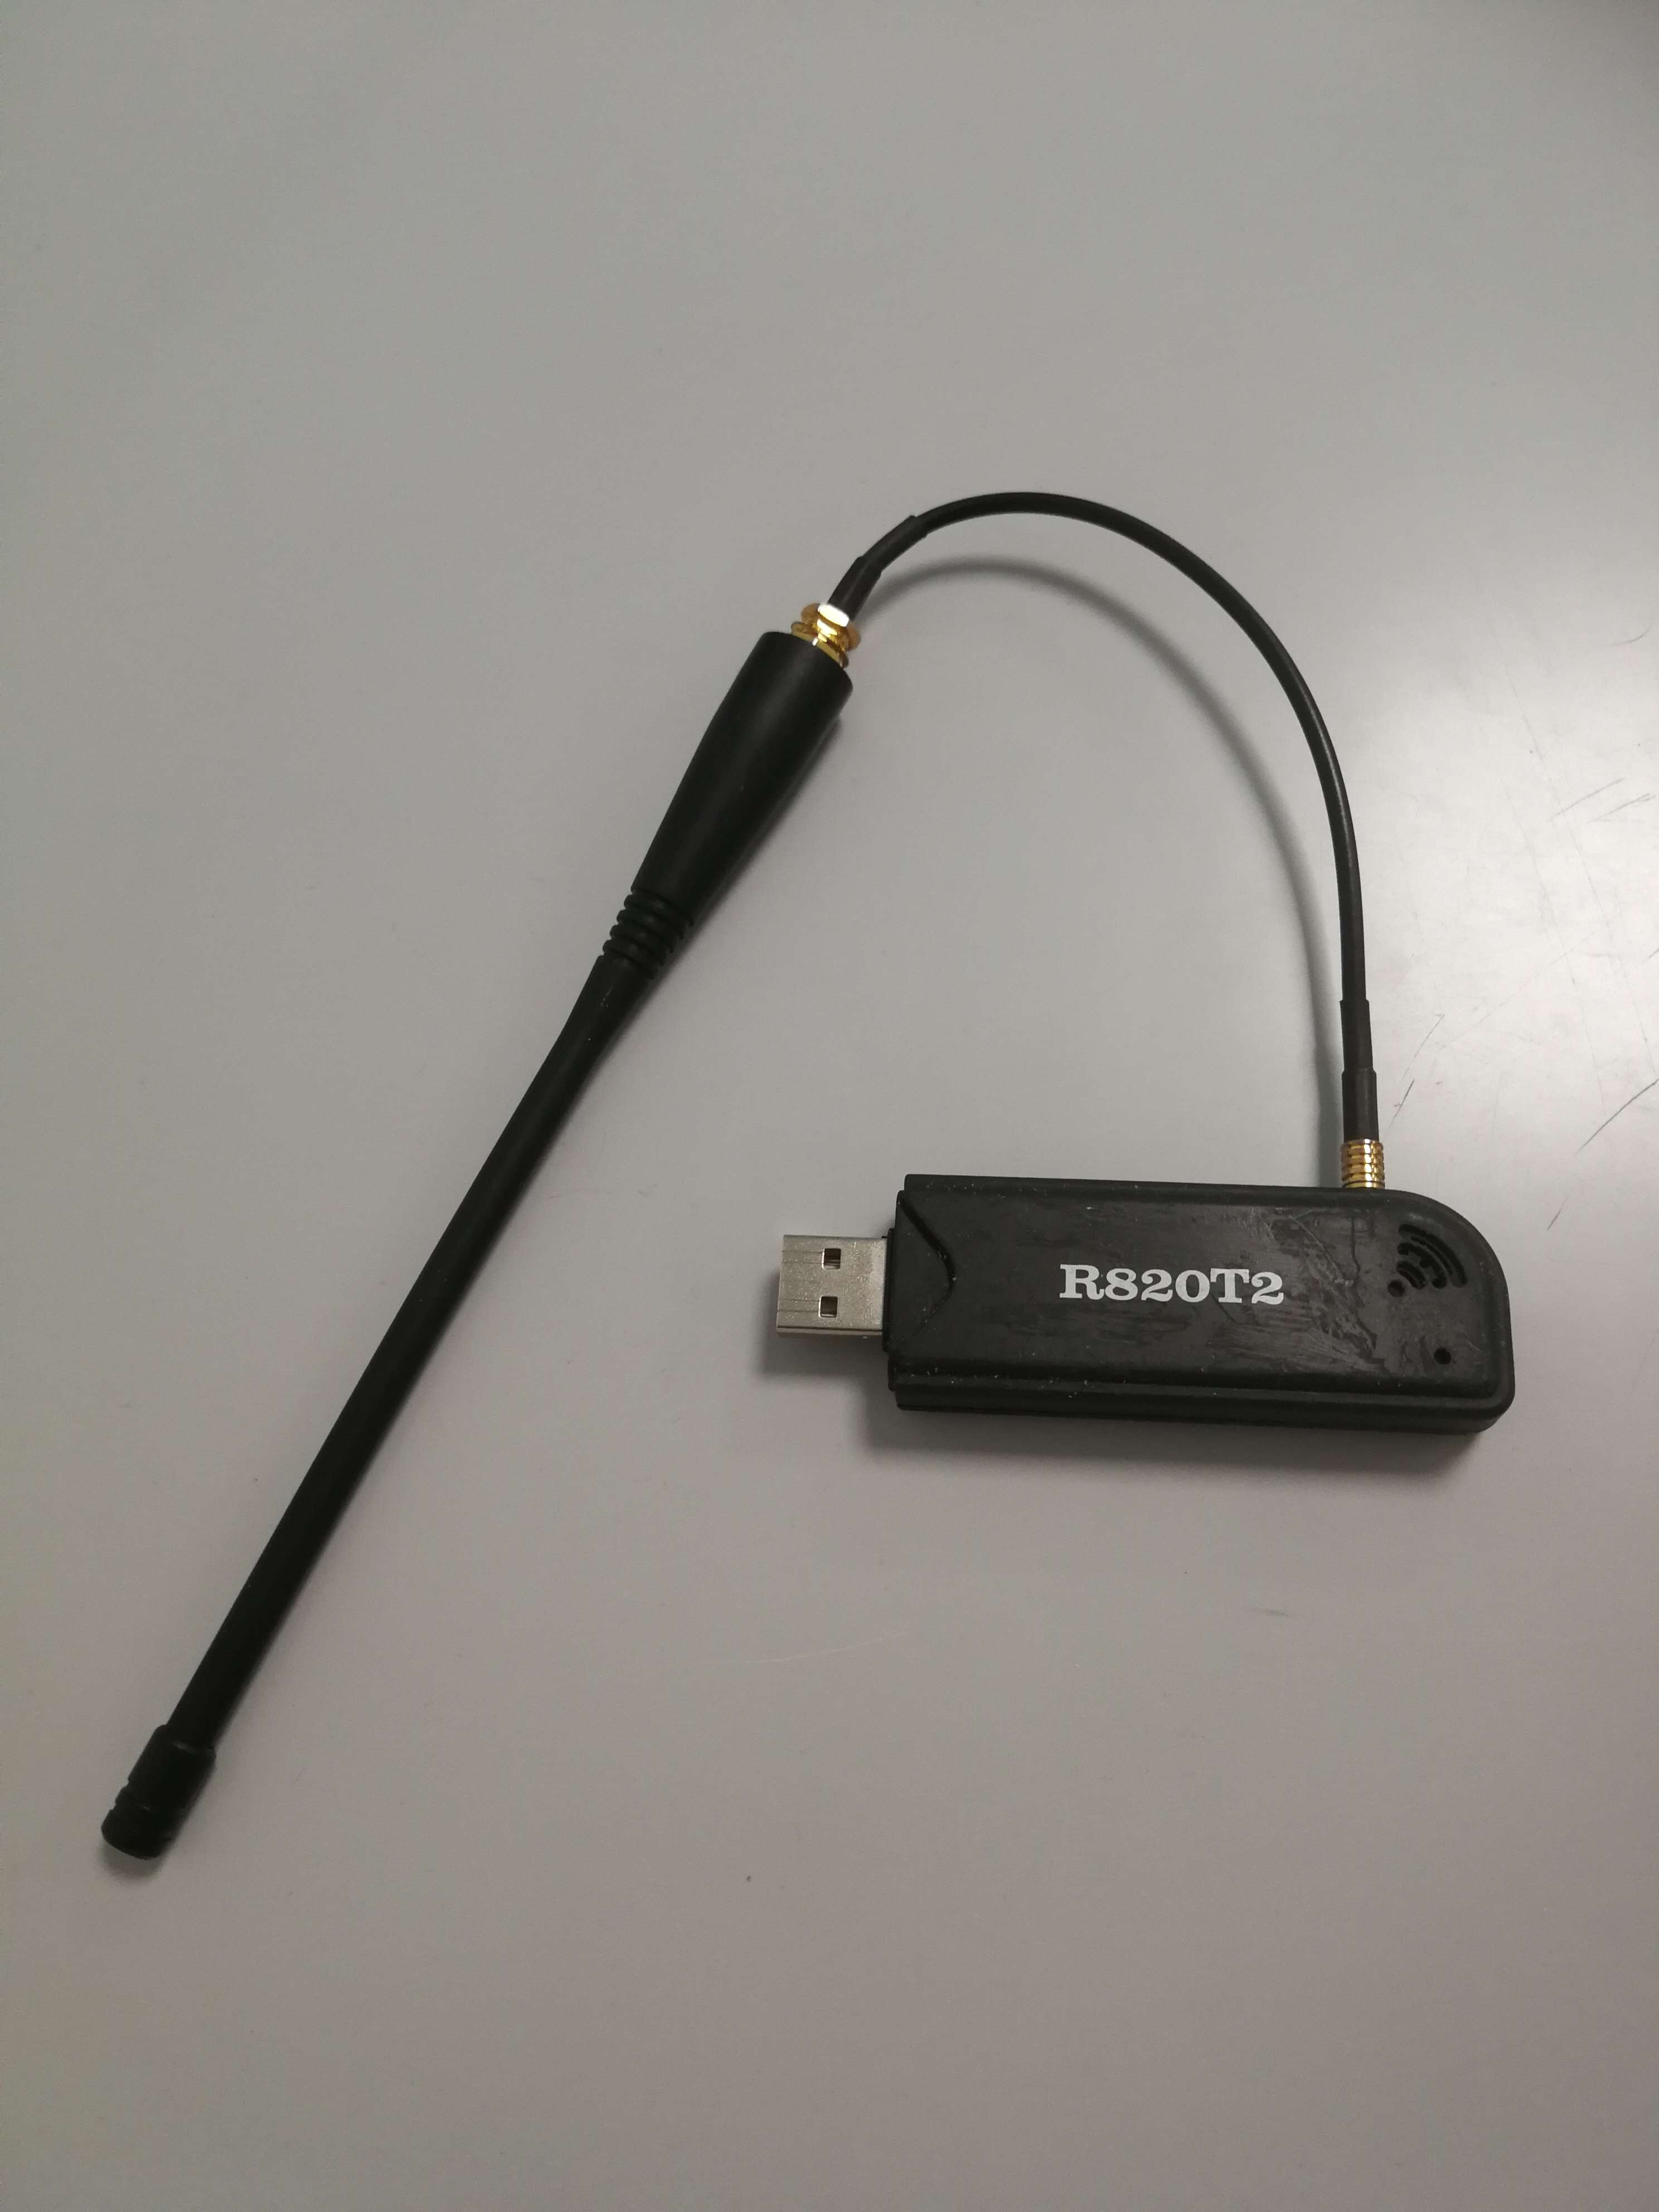
\includegraphics[scale=0.08]{images/r820t2.png}
\caption{RTL SDR R820T2}\label{term32}
\end{figure}

La deuxième radio logicielle utilisée est la \textit{RTL SDR R820T2}. Il y a deux différences majeures avec la radio DVB-T. L'antenne de cette radio logicielle est de meilleure qualité et le tuner chip de cette SDR est un R820T2. Cette version est une version améliorée du tuner qui se trouve dans la dvb-T, ce qui a pour impact une réduction du bruit, une meilleure sensibilité et une couverture de fréquence plus large. La figure \ref{term32} montre la SDR en question. Le schéma bloc de la SDR présentée à la section \ref{dvbt} est le même que pour celui-ci. En effet la différence entre le tuner T et T2 n'est pas visible sur la description du shéma. Une description détaillée de la RTL-SDR R820T2 est disponible sur le site RTL-SDR \footnote{Datasheet R820T2 : \href{https://www.rtl-sdr.com/wp-content/uploads/2013/04/R820T_datasheet-Non_R-20111130_unlocked1.pdf}{https://www.rtl-sdr.com/wp-content/uploads/2013/04/R820T-datasheet-Non-R-20111130-unlocked1.pdf}}


\subsubsection{HackRF One}

La dernière radio logicielle utilisée est la \textit{HackRF One}. Au dela du prix plus élevé, cette dernière radio est différente des deux autres. Elle est notamment capable de gérer la transmission et la réception de signaux, les deux autres sont uniquement des récepteurs. Si la R820T2 offrait déjà une qualité de signal supérieure à la DVB-T, celui de la HackRF est encore plus net. La figure \ref{bothimages} montre la SDR avec l'antenne utilisée montée sur un trépied.

\begin{figure}[h]
\centering
\begin{subfigure}{0.4\textwidth}
  \centering
  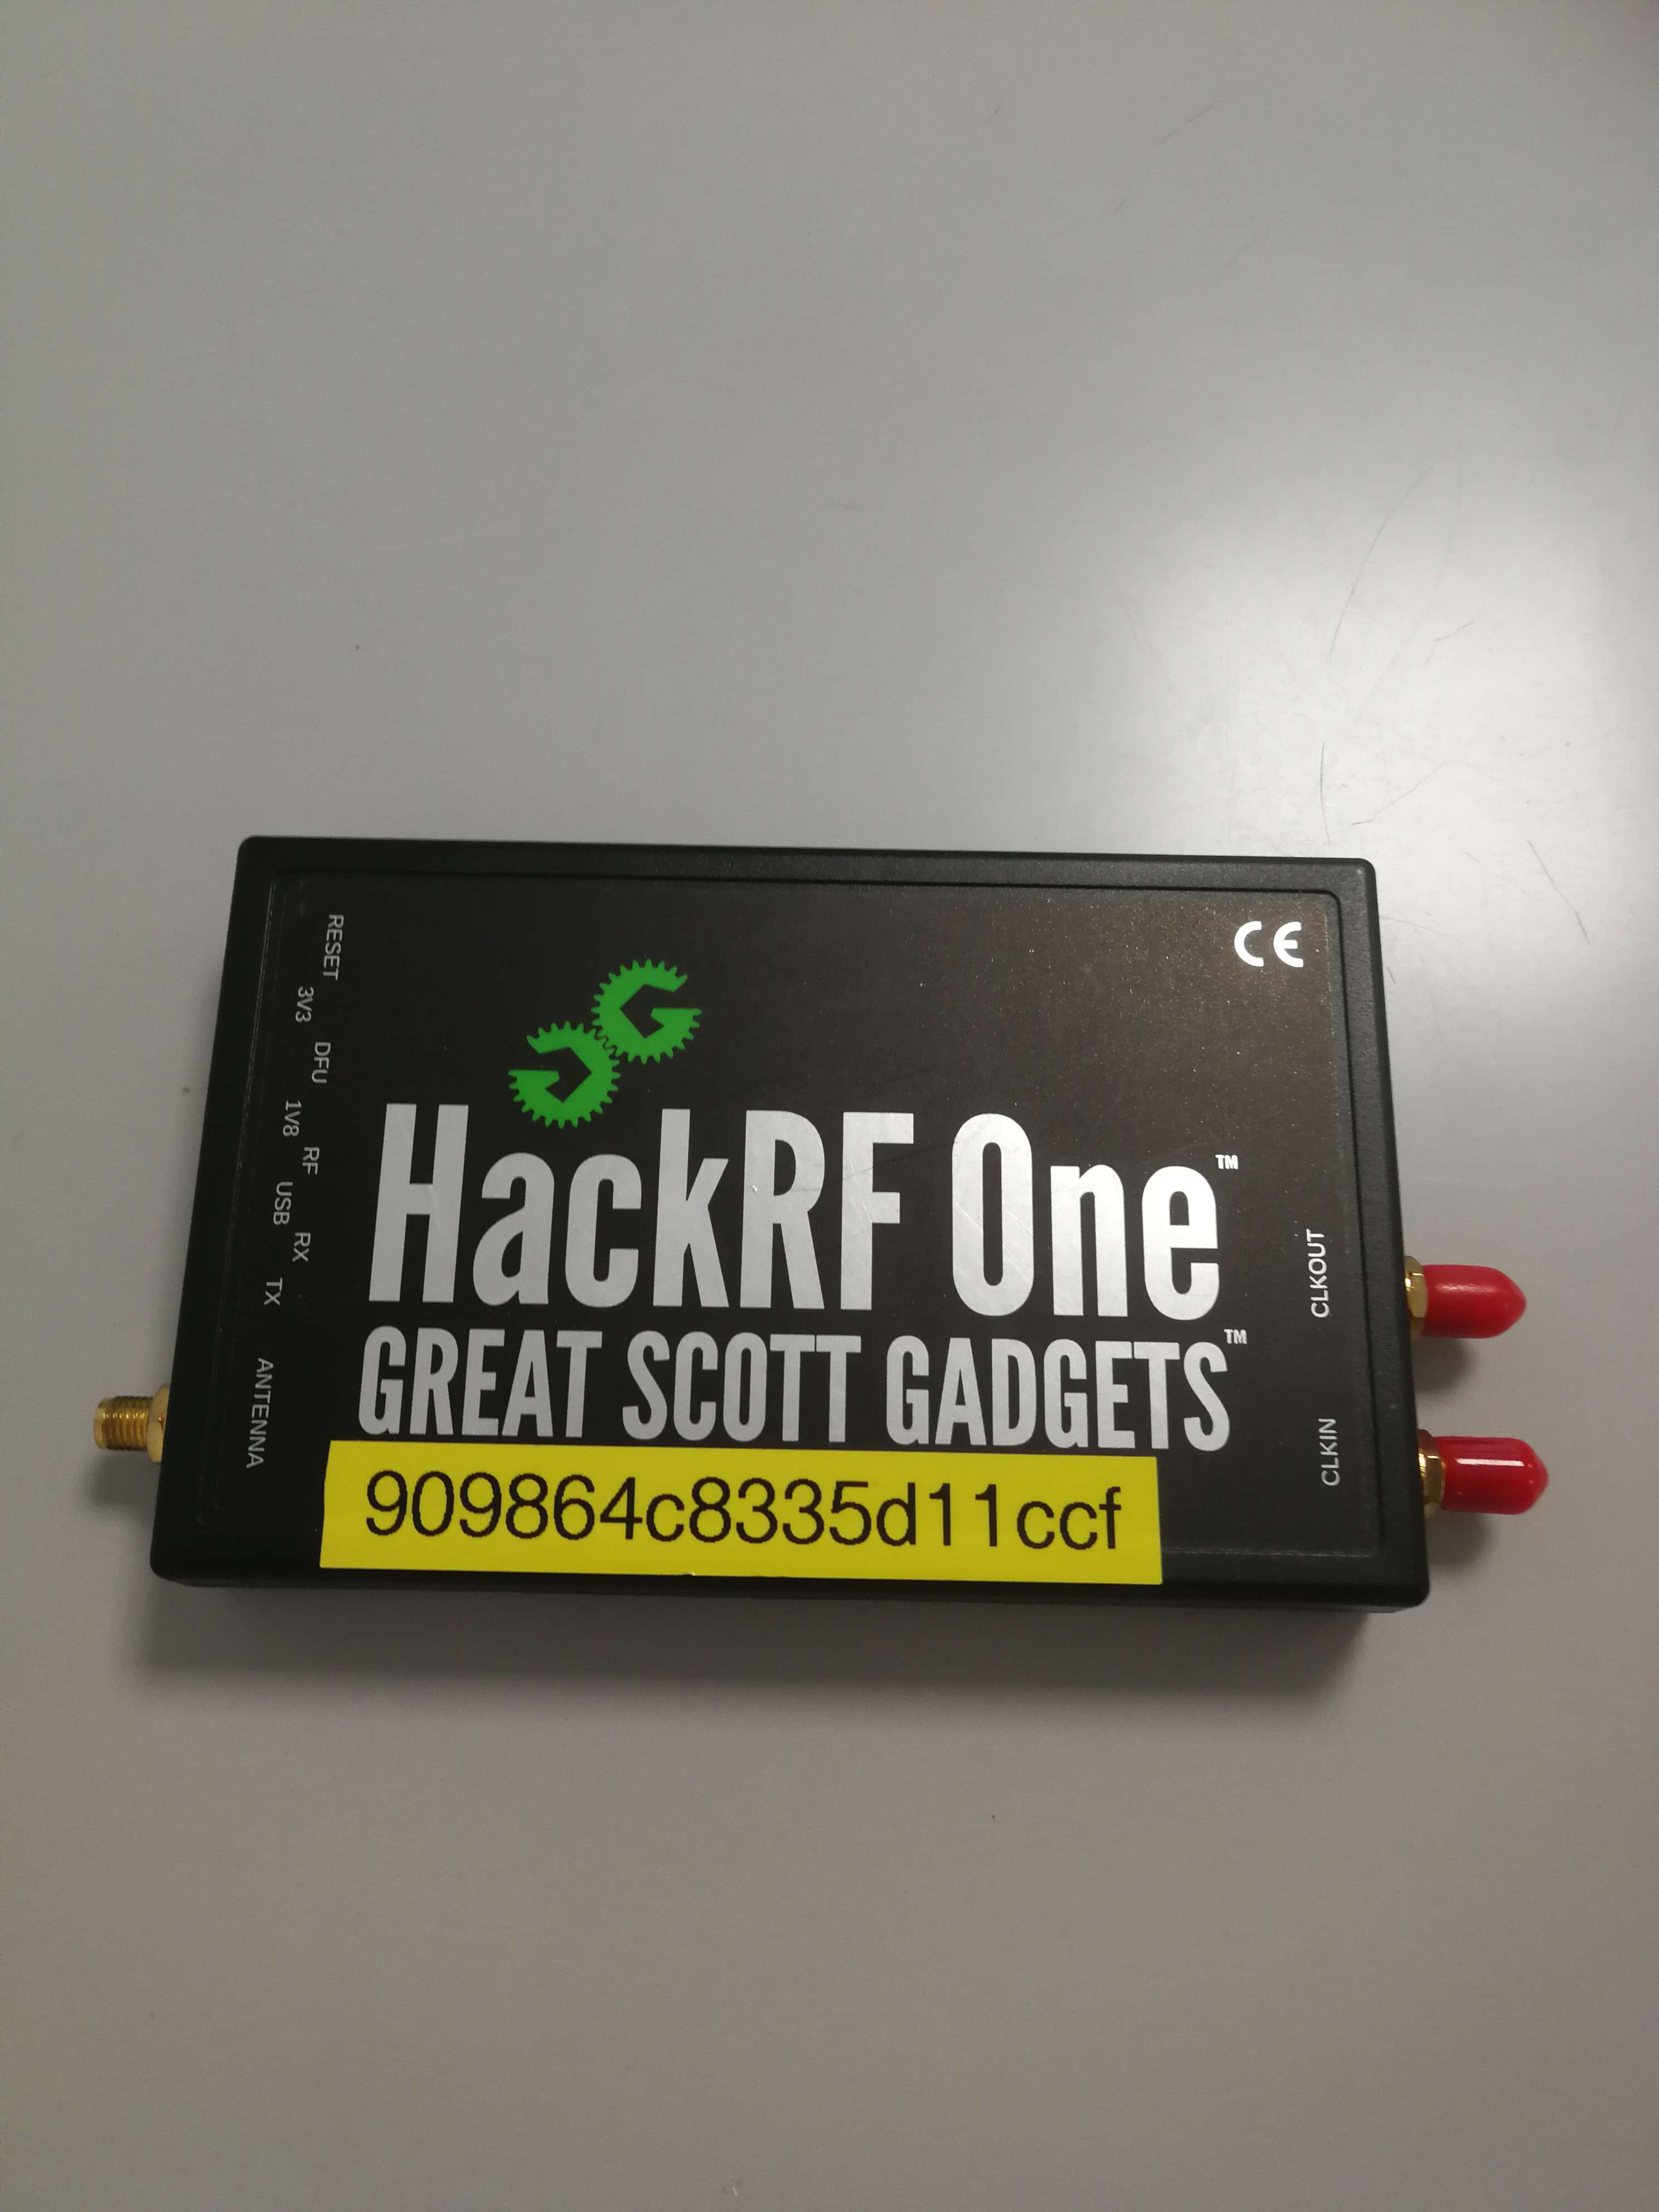
\includegraphics[width=\textwidth]{images/hackrf.png}
  \caption{SDR HackRF One}
  \label{term330}
\end{subfigure}
\hspace{0.5cm} % Adjust the horizontal space between the subfigures
\begin{subfigure}{0.4\textwidth}
  \centering
  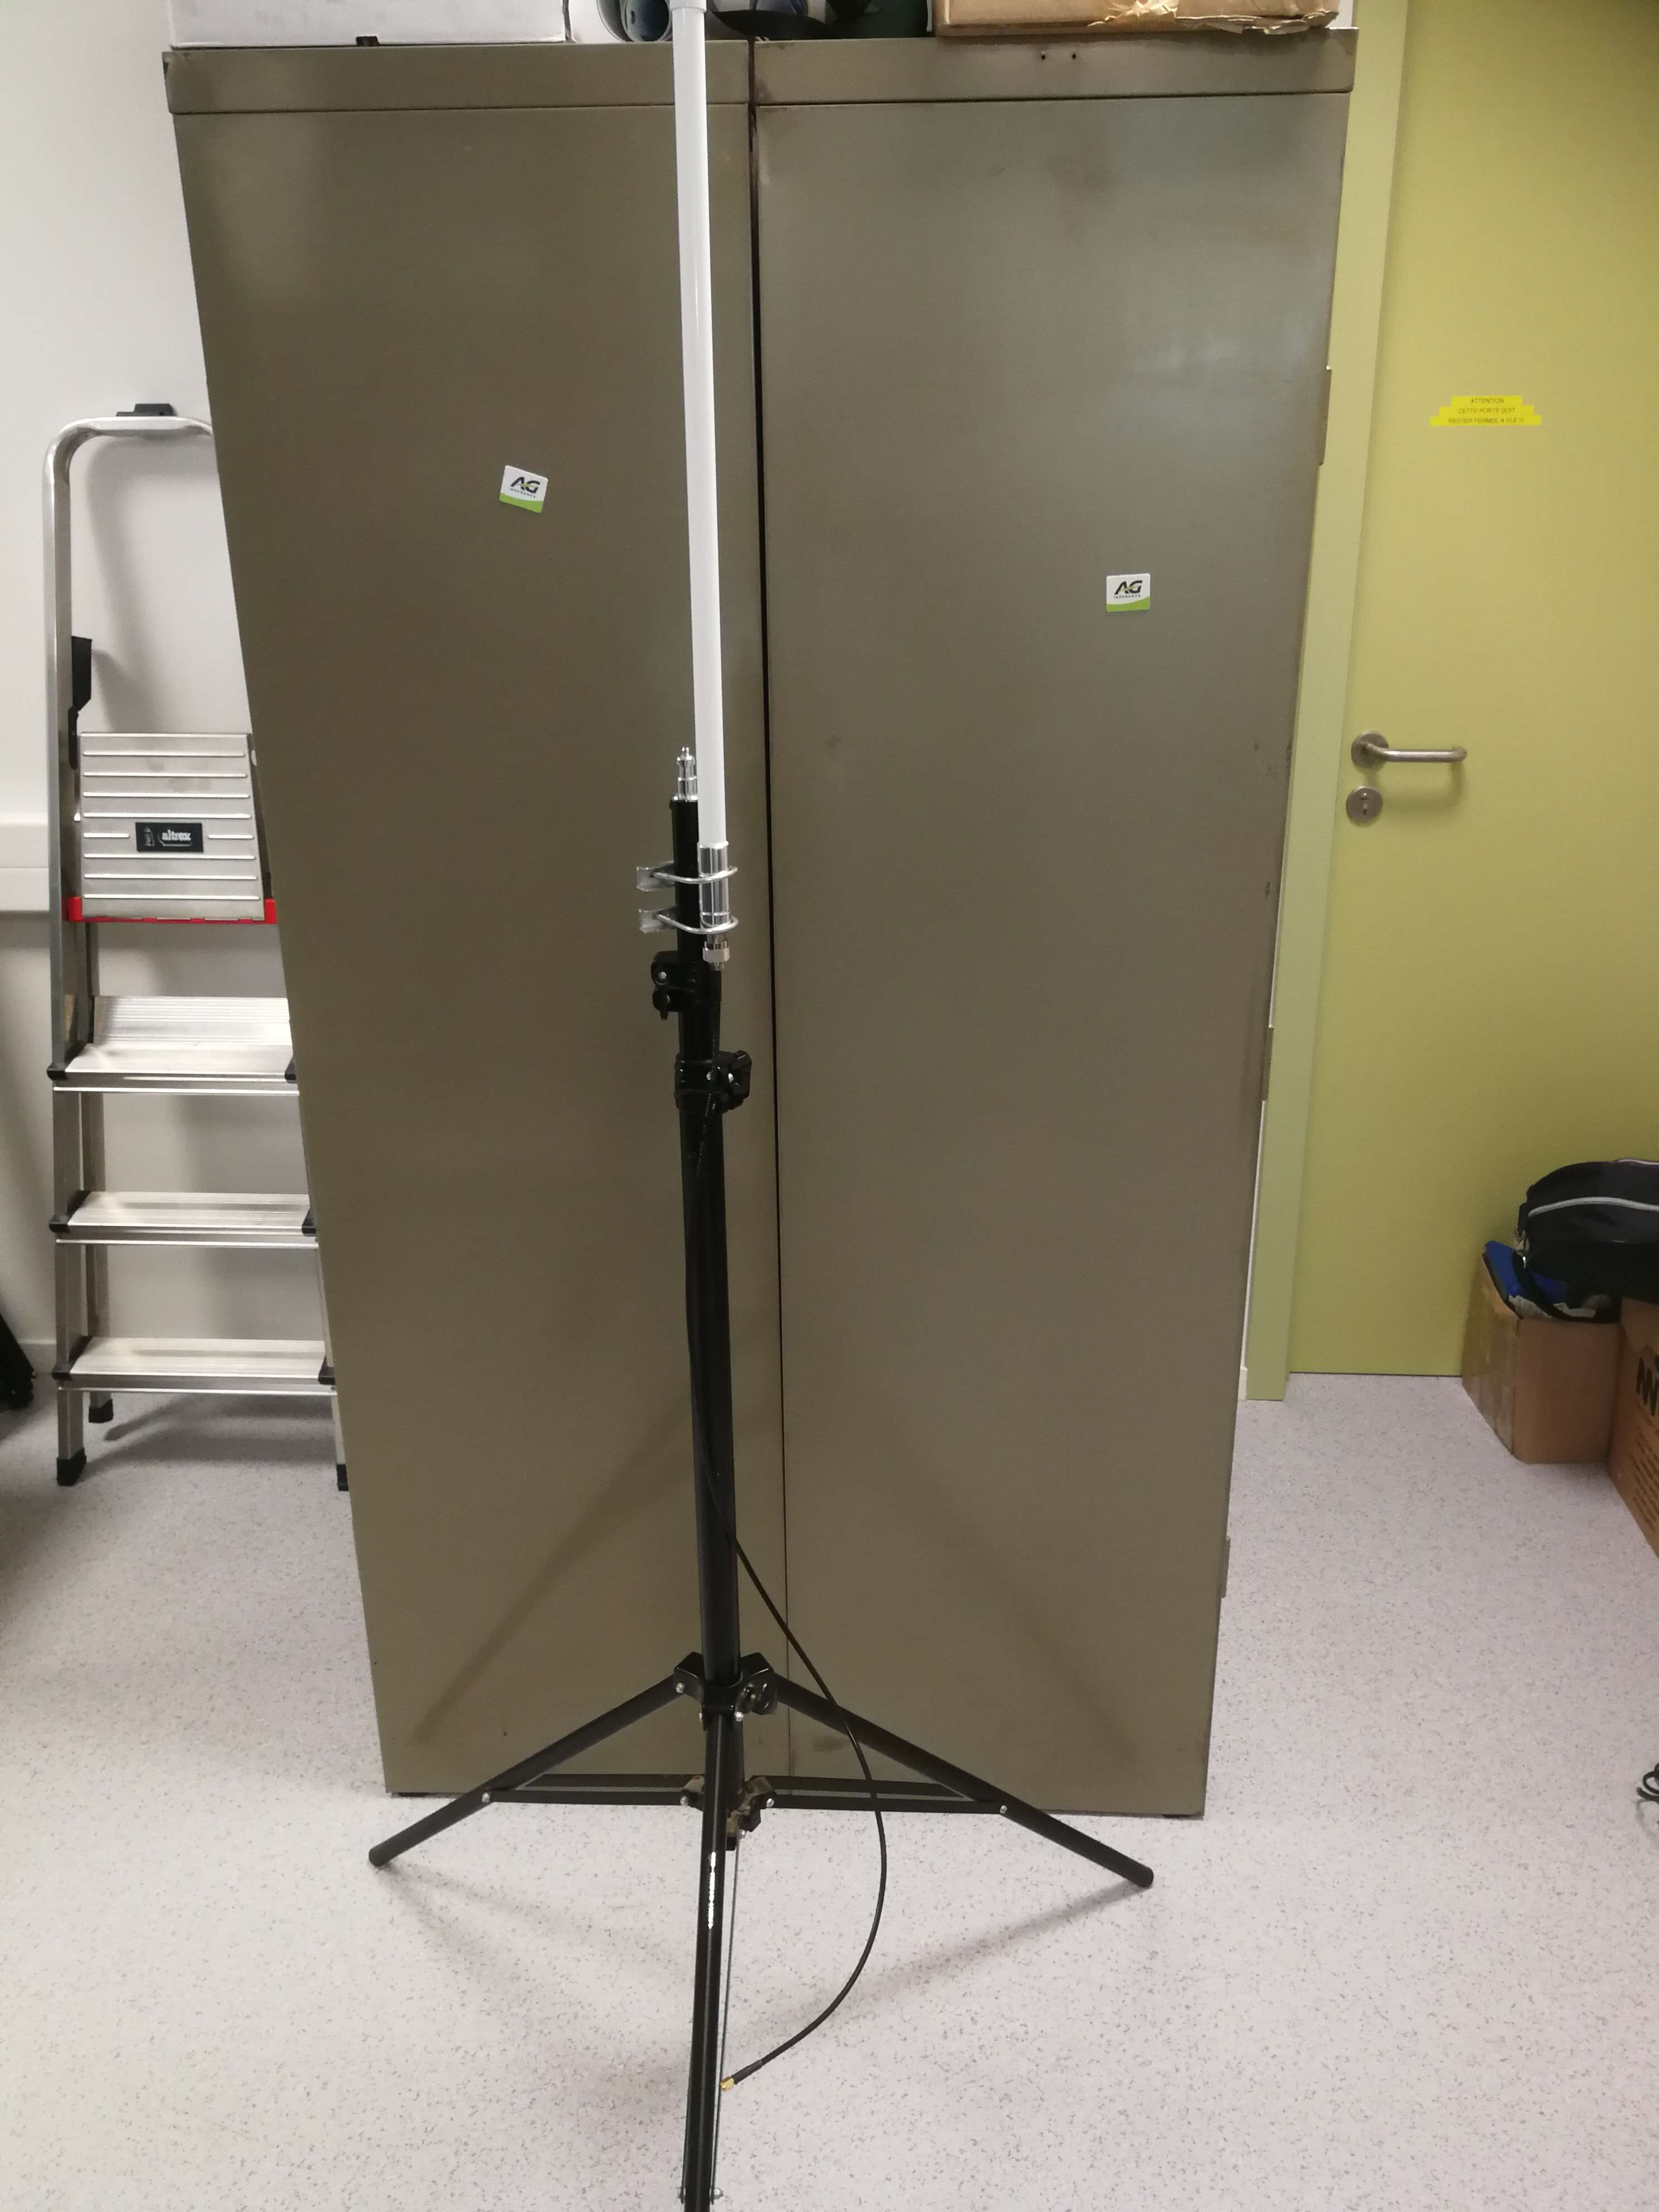
\includegraphics[width=\textwidth]{images/pied.png}
  \caption{Antenne}
  \label{term340}
\end{subfigure}
\caption{SDR HackRf One avec son antenne}
\label{bothimages}
\end{figure}


Le schéma bloc de la SDR est affiché sur la figure \ref{term3001}. Ce dernier est beaucoup plus complexe que celui de la RTL SDR. Il y a d'une part que la HackRF est un transceiver, donc elle possède les étapes nécessaires à l'émission que la RTL SDR ne possède pas. Ensuite, il y a plusieurs étapes de fréquences intermédiaires. L'architecture de la HackRF \footnotemark[10] permet d'utiliser plusieurs étapes de mixeur pour atteindre la fréquence désirée. Chaque étape possède sa fréquence intermédiaire.

\begin{figure}[h]
\centering

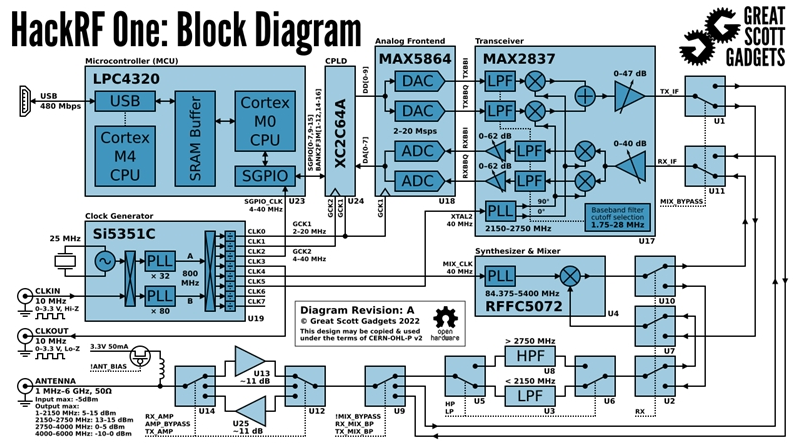
\includegraphics[scale=0.8]{images/SBhackrf.png}
\caption{Schéma bloc de la HackRF One\protect\footnotemark[10]}\label{term3001}
\end{figure}

\footnotetext[10]{HackRF One : \href{https://www.hb9afo.ch/articles/HackRF/default.htm}{https://www.hb9afo.ch/articles/HackRF/default.htm}}
 
La table \ref{table1} résume les différents critères pertinents pour les trois radios logicielles. Ces critères permettront de sélectionner la SDR la plus adéquate pour les expérimentations.


\begin{table}[h]
\centering
\begin{adjustbox}{width=1\textwidth}
\begin{tabular}{|c|c|c|c|}
\hline
\multicolumn{1}{|c|}{Caractéristiques importantes} & \multicolumn{1}{c|}{RTL SDR DVB-T} & \multicolumn{1}{c|}{RTL SDR R820T2} & \multicolumn{1}{c|}{HackRF One}\\
\hline
Portée (Fréquence) & \multicolumn{2}{c|}{24MHz - 1.7GHz} & 1MHz - 6GHz \\
\hline
Taux d'échantillonnage & \multicolumn{2}{c|}{jusqu'à 3.2MHz} & jusqu'à 20MHz \\
\hline
Largeur de bande & \multicolumn{2}{c|}{jusqu'à 2.4MHz} & jusqu'à 20MHz  \\
\hline
Résolutions de l'ADC & \multicolumn{3}{c|}{8 bits} \\
\hline
RX & \multicolumn{3}{c|}{oui} \\
\hline
TX & \multicolumn{2}{c|}{non} & oui \\
\hline
Compatibilié logicielle & \multicolumn{3}{c|}{oui, notamment avec ceux décrits dans la section \ref{fft}} \\
\hline
Qualité du signal & mauvaise &\multicolumn{2}{c|}{très bonne}\\
\hline
Prix & $+-$ 20 euros & $+-$ 30 euros & $>$ 250 euros \\
\hline
\end{tabular}
\end{adjustbox}
\caption{Table comparative des radios logicielles utilisées}
\label{table1}
\end{table}



\subsection{Module d'émission Lora}

La transmission de signaux via la technologie LoRa est un aspect essentiel du travail. Afin de garantir la meilleure qualité de transmission possible, différents modules sont testés. Cela permet de distinguer les variations de performance et de capacitées entre les modules. Certains modules sont plus facilement configurable que d'autres, et d'autres nécessitent des composants hardware ou software spécifiques.

\subsubsection{Module RN2483}

\begin{figure}[h]
\centering

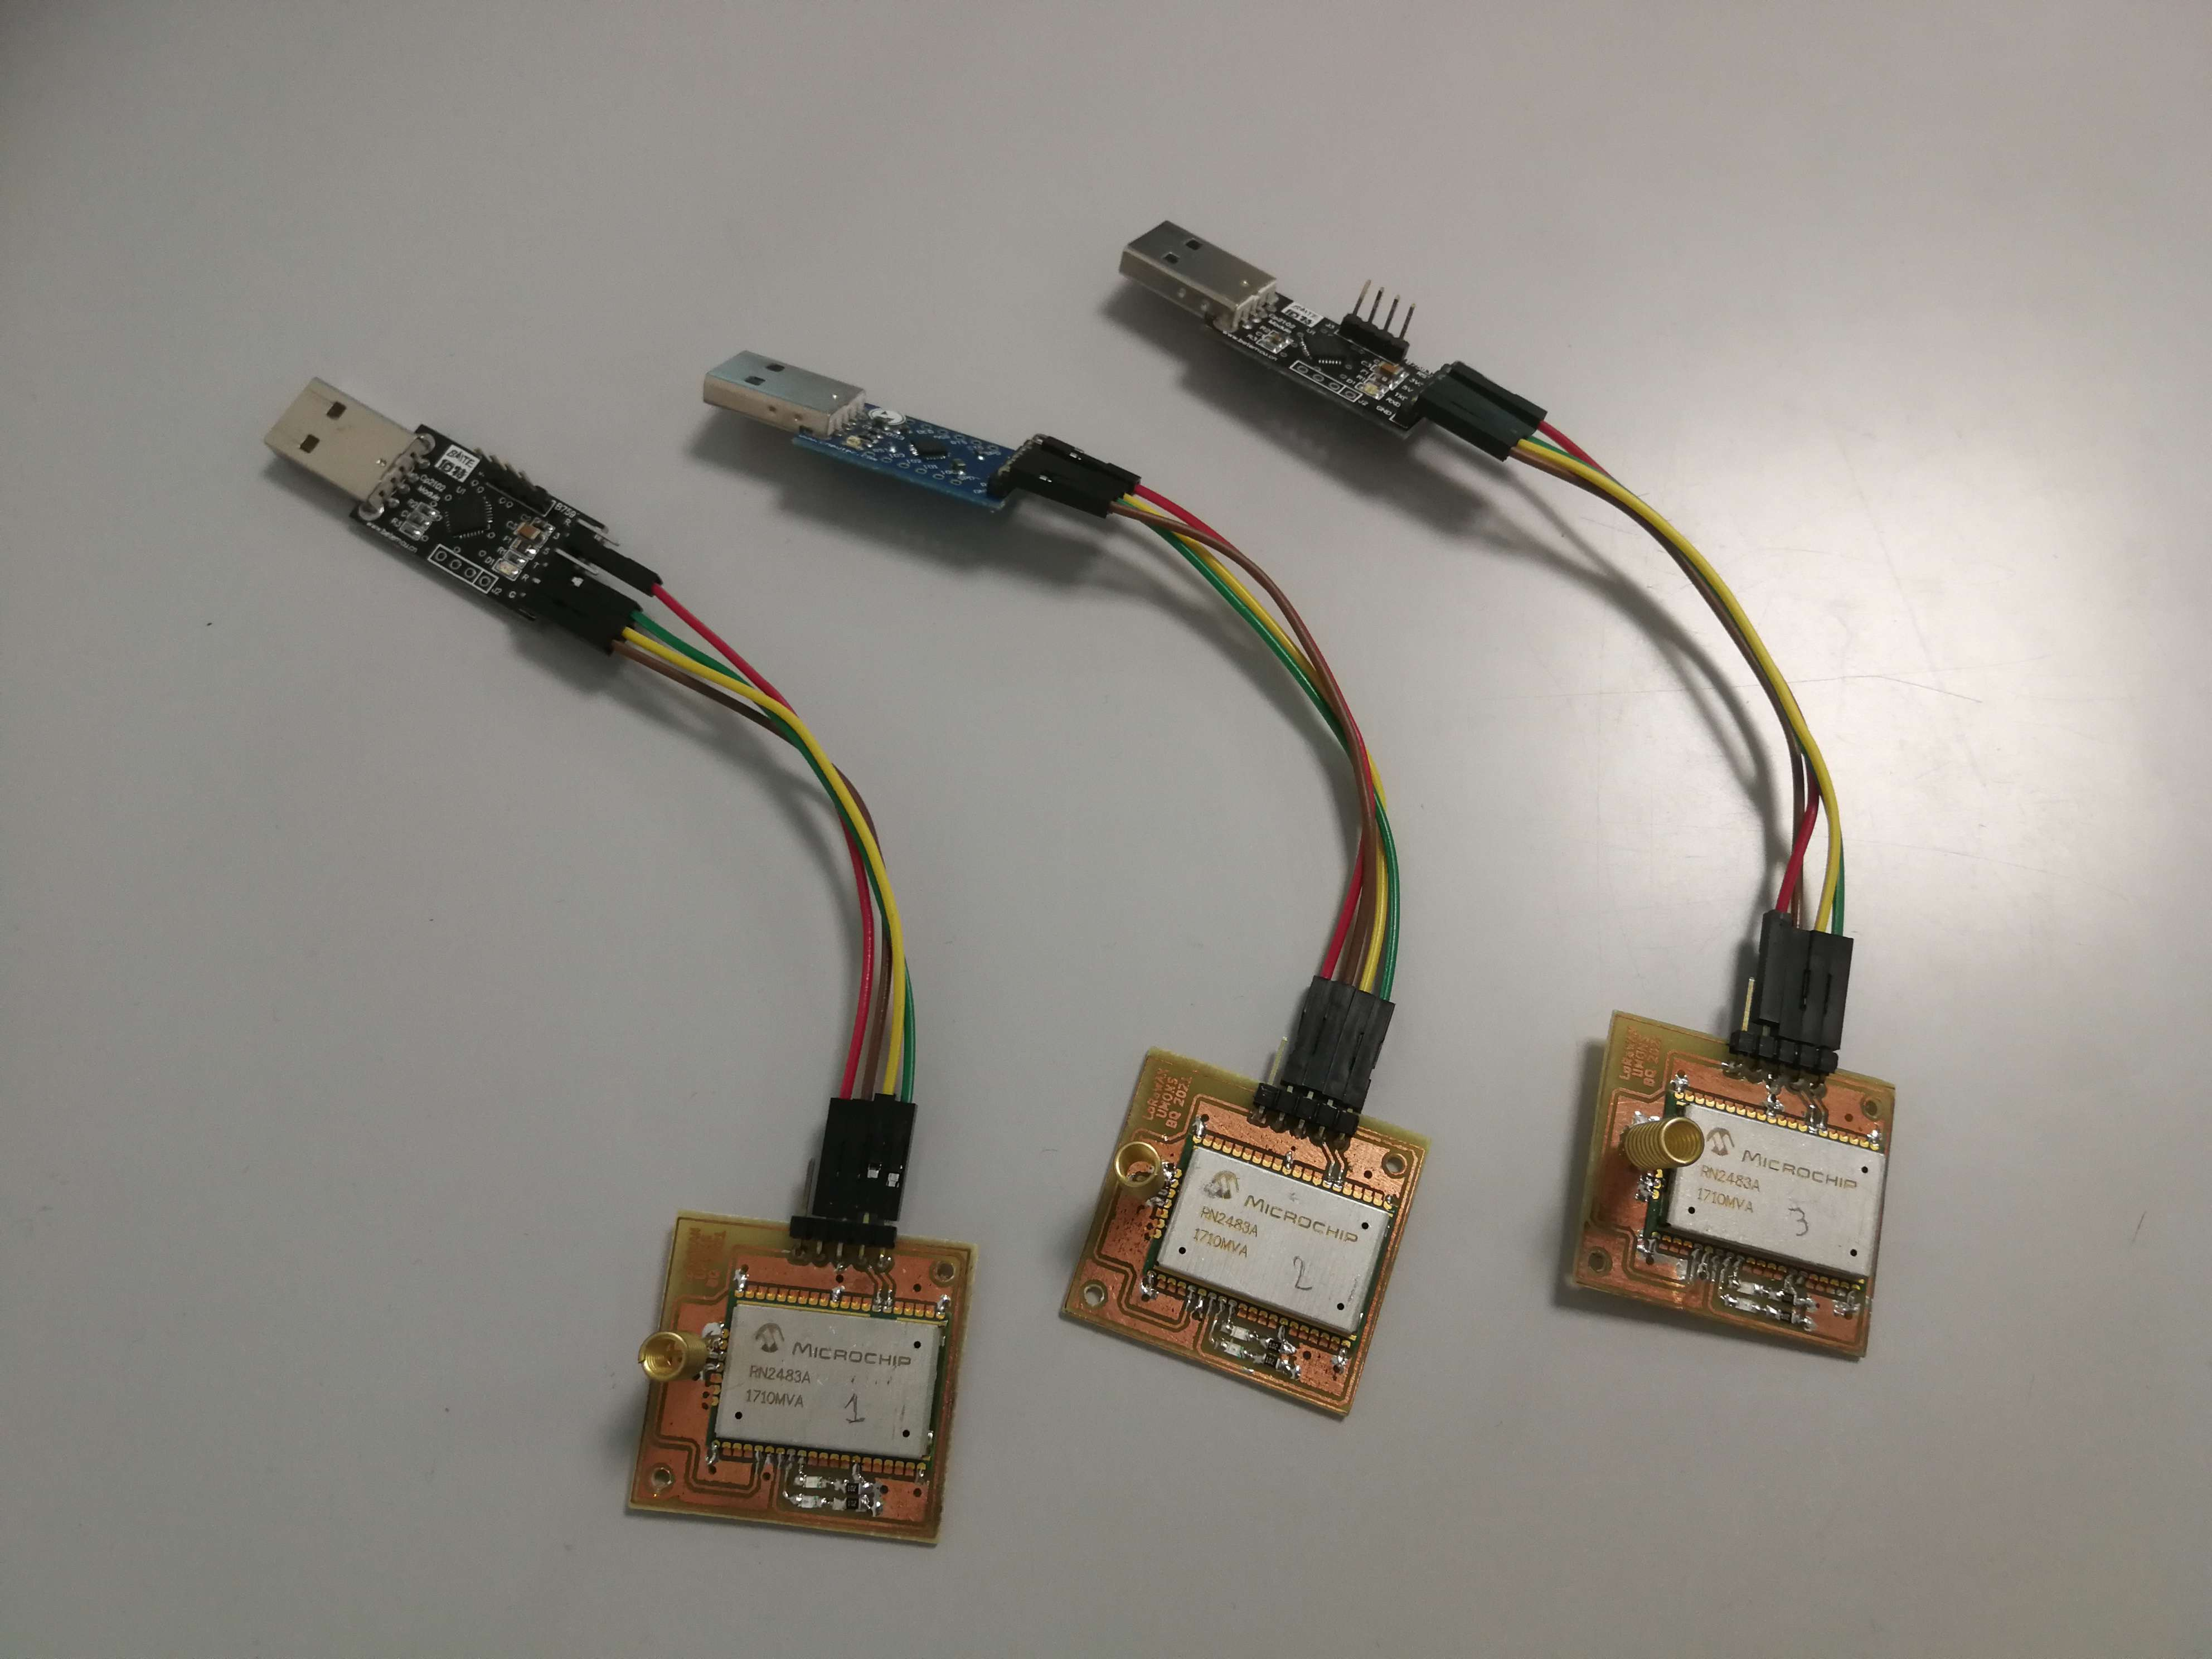
\includegraphics[scale=0.08]{images/rn2483.png}
\caption{3 modules RN2483}\label{term34}
\end{figure}


Le \textit{microchip RN2483}\footnote{Datasheet RN2483 :\href{https://ww1.microchip.com/downloads/en/DeviceDoc/40001784B.pdf}{https://ww1.microchip.com/downloads
/en/DeviceDoc/}} est un module de technologie spécifique à LoRa permettant de communiquer à longue portée et à faible coup. Le Schéma bloc \footnote{Shéma bloc rn2483 : \href{https://www.mouser.be/new/microchip/microchip-rn2483-module/}{https://www.mouser.be/new/microchip/microchip-rn2483-module/}} du module est représenté à la figure \ref{term3002}. Le module RN2483 de la figure \ref{term34} est un simple \textit{transceiver (transmitter and receiver)} radio de type SX127x couplé à un microcontroleur. Les informations relatives à ce type de transceivers sont disponibles sur le site de Semtech \footnote{Semtech : \href{https://www.semtech.com/products/wireless-rf/lora-connect/sx1278}{https://www.semtech.com/products/wireless-rf/lora-connect/sx1278}}.


Voici quelques spécificités du module:
\vspace{0.1cm}

\begin{itemize}
\item Il comprend la technologie de modulation LoRa, ce qui lui donne son atout de faible consommation et de longue portée. Il gère également les modulations \textit{FSK (frequency shift keying)} et \textit{GFSK (Gaussian frequency shift keying)}.
\item Une faible consommation induit une faible puissance, le module possède un amplificateur de puissance maximale de 14dBm.
\item Les bandes de fréquences disponibles sont compatibles avec la bande ISM. Le module couvre de 863Mhz à 870Mhz pour la région européenne.
\item Le data rate maximum en modulant avec LoRa est de 27343.75 bps (bit par seconde) pour un largeur de bande de 125KHz et un facteur d'étalement de 7.
\item tous les paramètres TX sont configurables.
\end{itemize}


\begin{figure}[h]
\centering

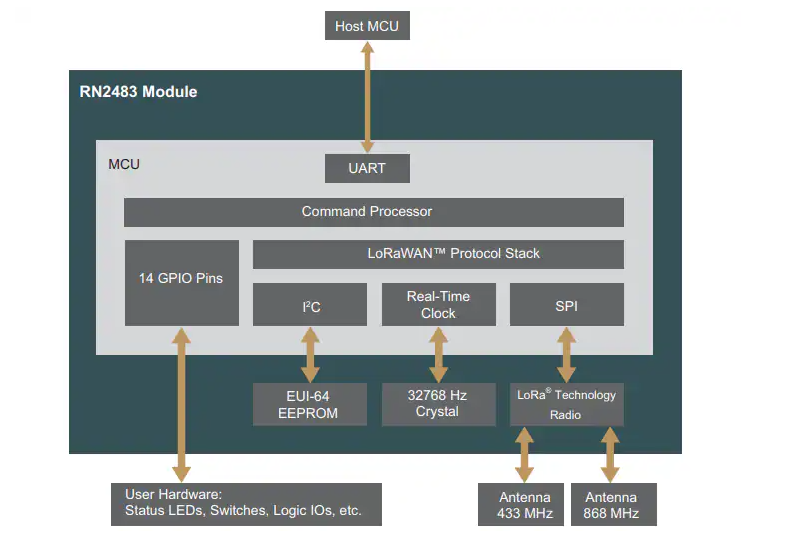
\includegraphics[scale=0.8]{images/SBrn2483.png}
\caption{Schéma bloc du module RN2483}\label{term3002}
\end{figure}

L'utilisation du module RN2483 est détaillée dans la section \ref{signallora}.

\subsubsection{Module Pycom LoPy}



Le module \textit{Pycom LoPy} \footnotemark[11] est un appareil programmable en micro python. Il comprend un microcontroleur ainsi qu'une série de pins digitaux input/output,  des composantes de connectivité sans fil et un port micro USB. La figure \ref{term35} montre le module  connecté à une antenne.

\newpage

\begin{figure}[h]
\centering

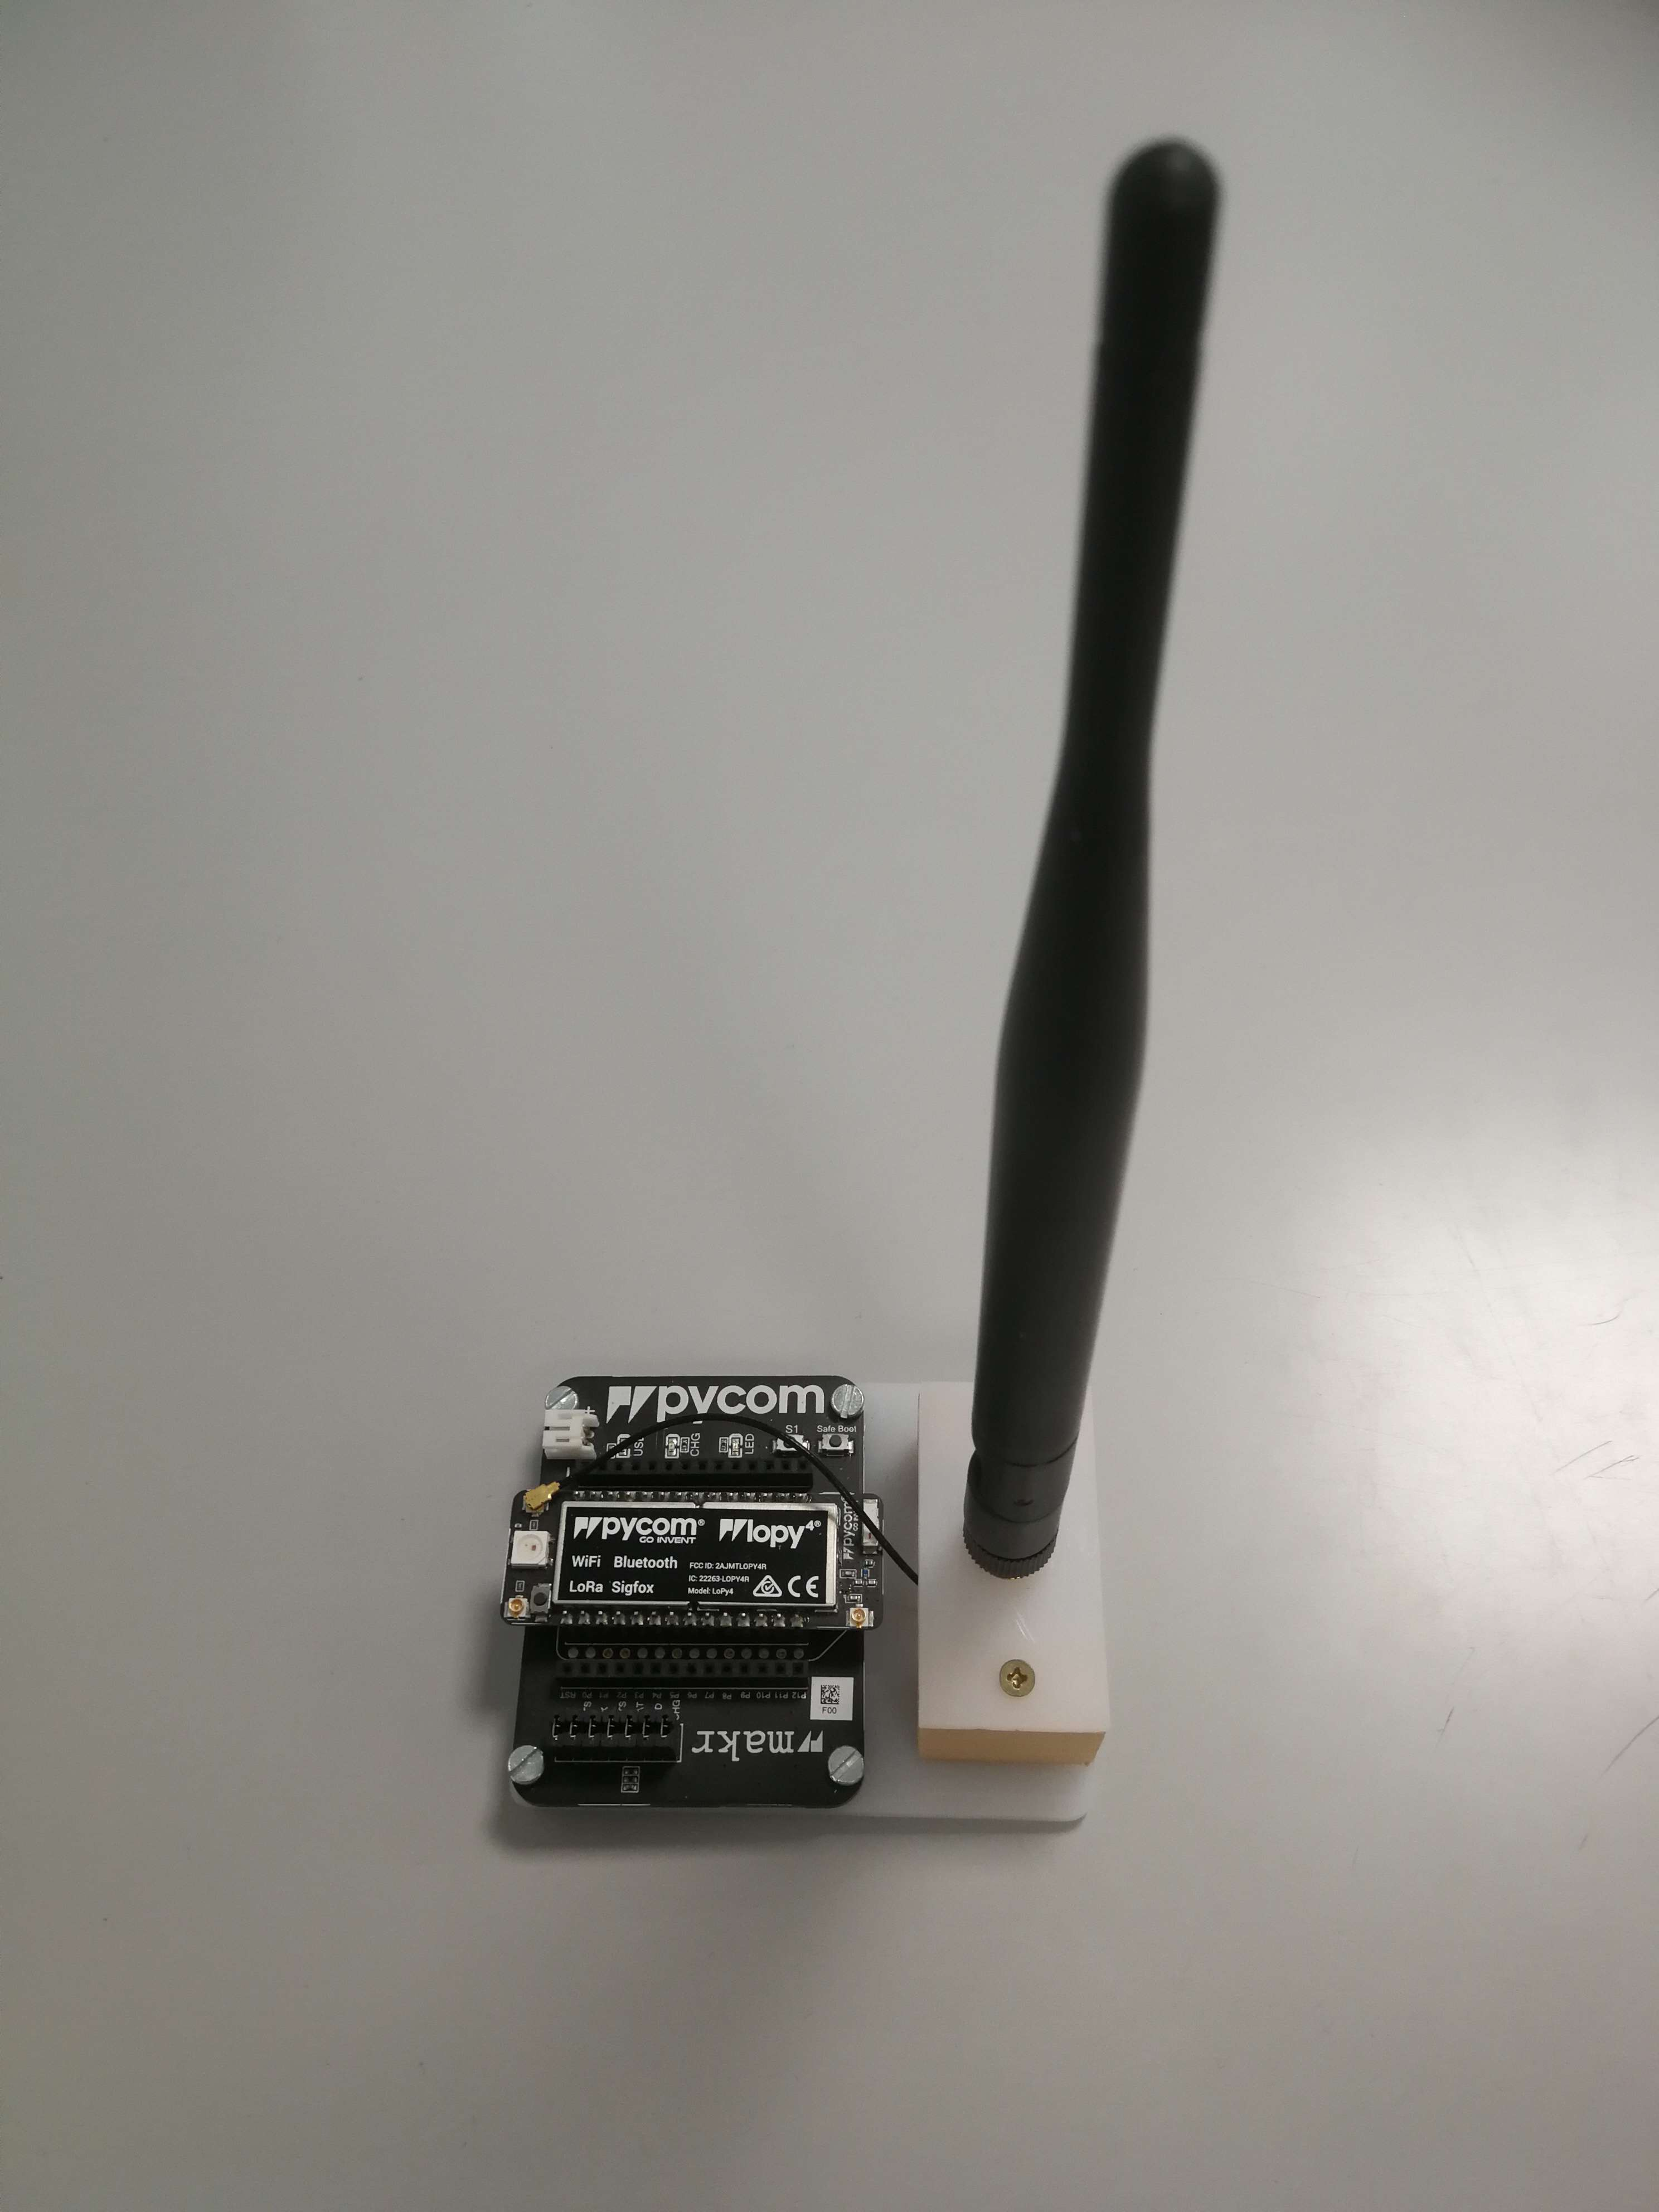
\includegraphics[scale=0.08]{images/lopy.png}
\caption{Un module Pycom lopy avec une antenne}\label{term35}
\end{figure}


Le shéma bloc \footnotemark[11]  est représenté à la figure \ref{term3003}. Contrairement au module RN2483, on remarque que le module LoPy possède des fonctions supplémentaires 
(qui ne sont pas intéressantes pour l'expérimentation) comme une connexion Wifi ou Bluetooth. Le microcontrolleur possède aussi plusieurs interfaces autres que UART (qui est la seul disponible sur le module RN42483).

\newpage

\begin{figure}[h]
\centering

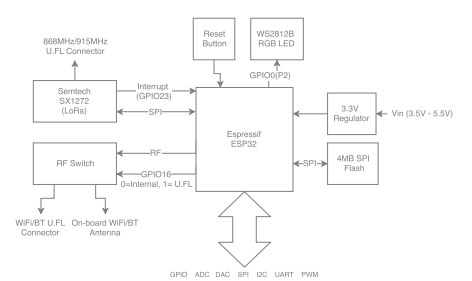
\includegraphics[scale=1]{images/SBlopy.png}
\caption{Schéma bloc du module Pycom LoPy \protect\footnotemark[11]}\label{term3003}
\end{figure}

\footnotetext[11]{Datasheet Pycom LoPy : \href{https://docs.pycom.io/gitbook/assets/specsheets/Pycom_002_Specsheets_LoPy_v2.pdf}{https://docs.pycom.io/gitbook/assets/specsheets/Pycom002SpecsheetsLoPyv2.pdf}}

\subsubsection{Module Arduino couplé à un transceiver LoRa}\label{arduino}

\begin{figure}[h]
\centering

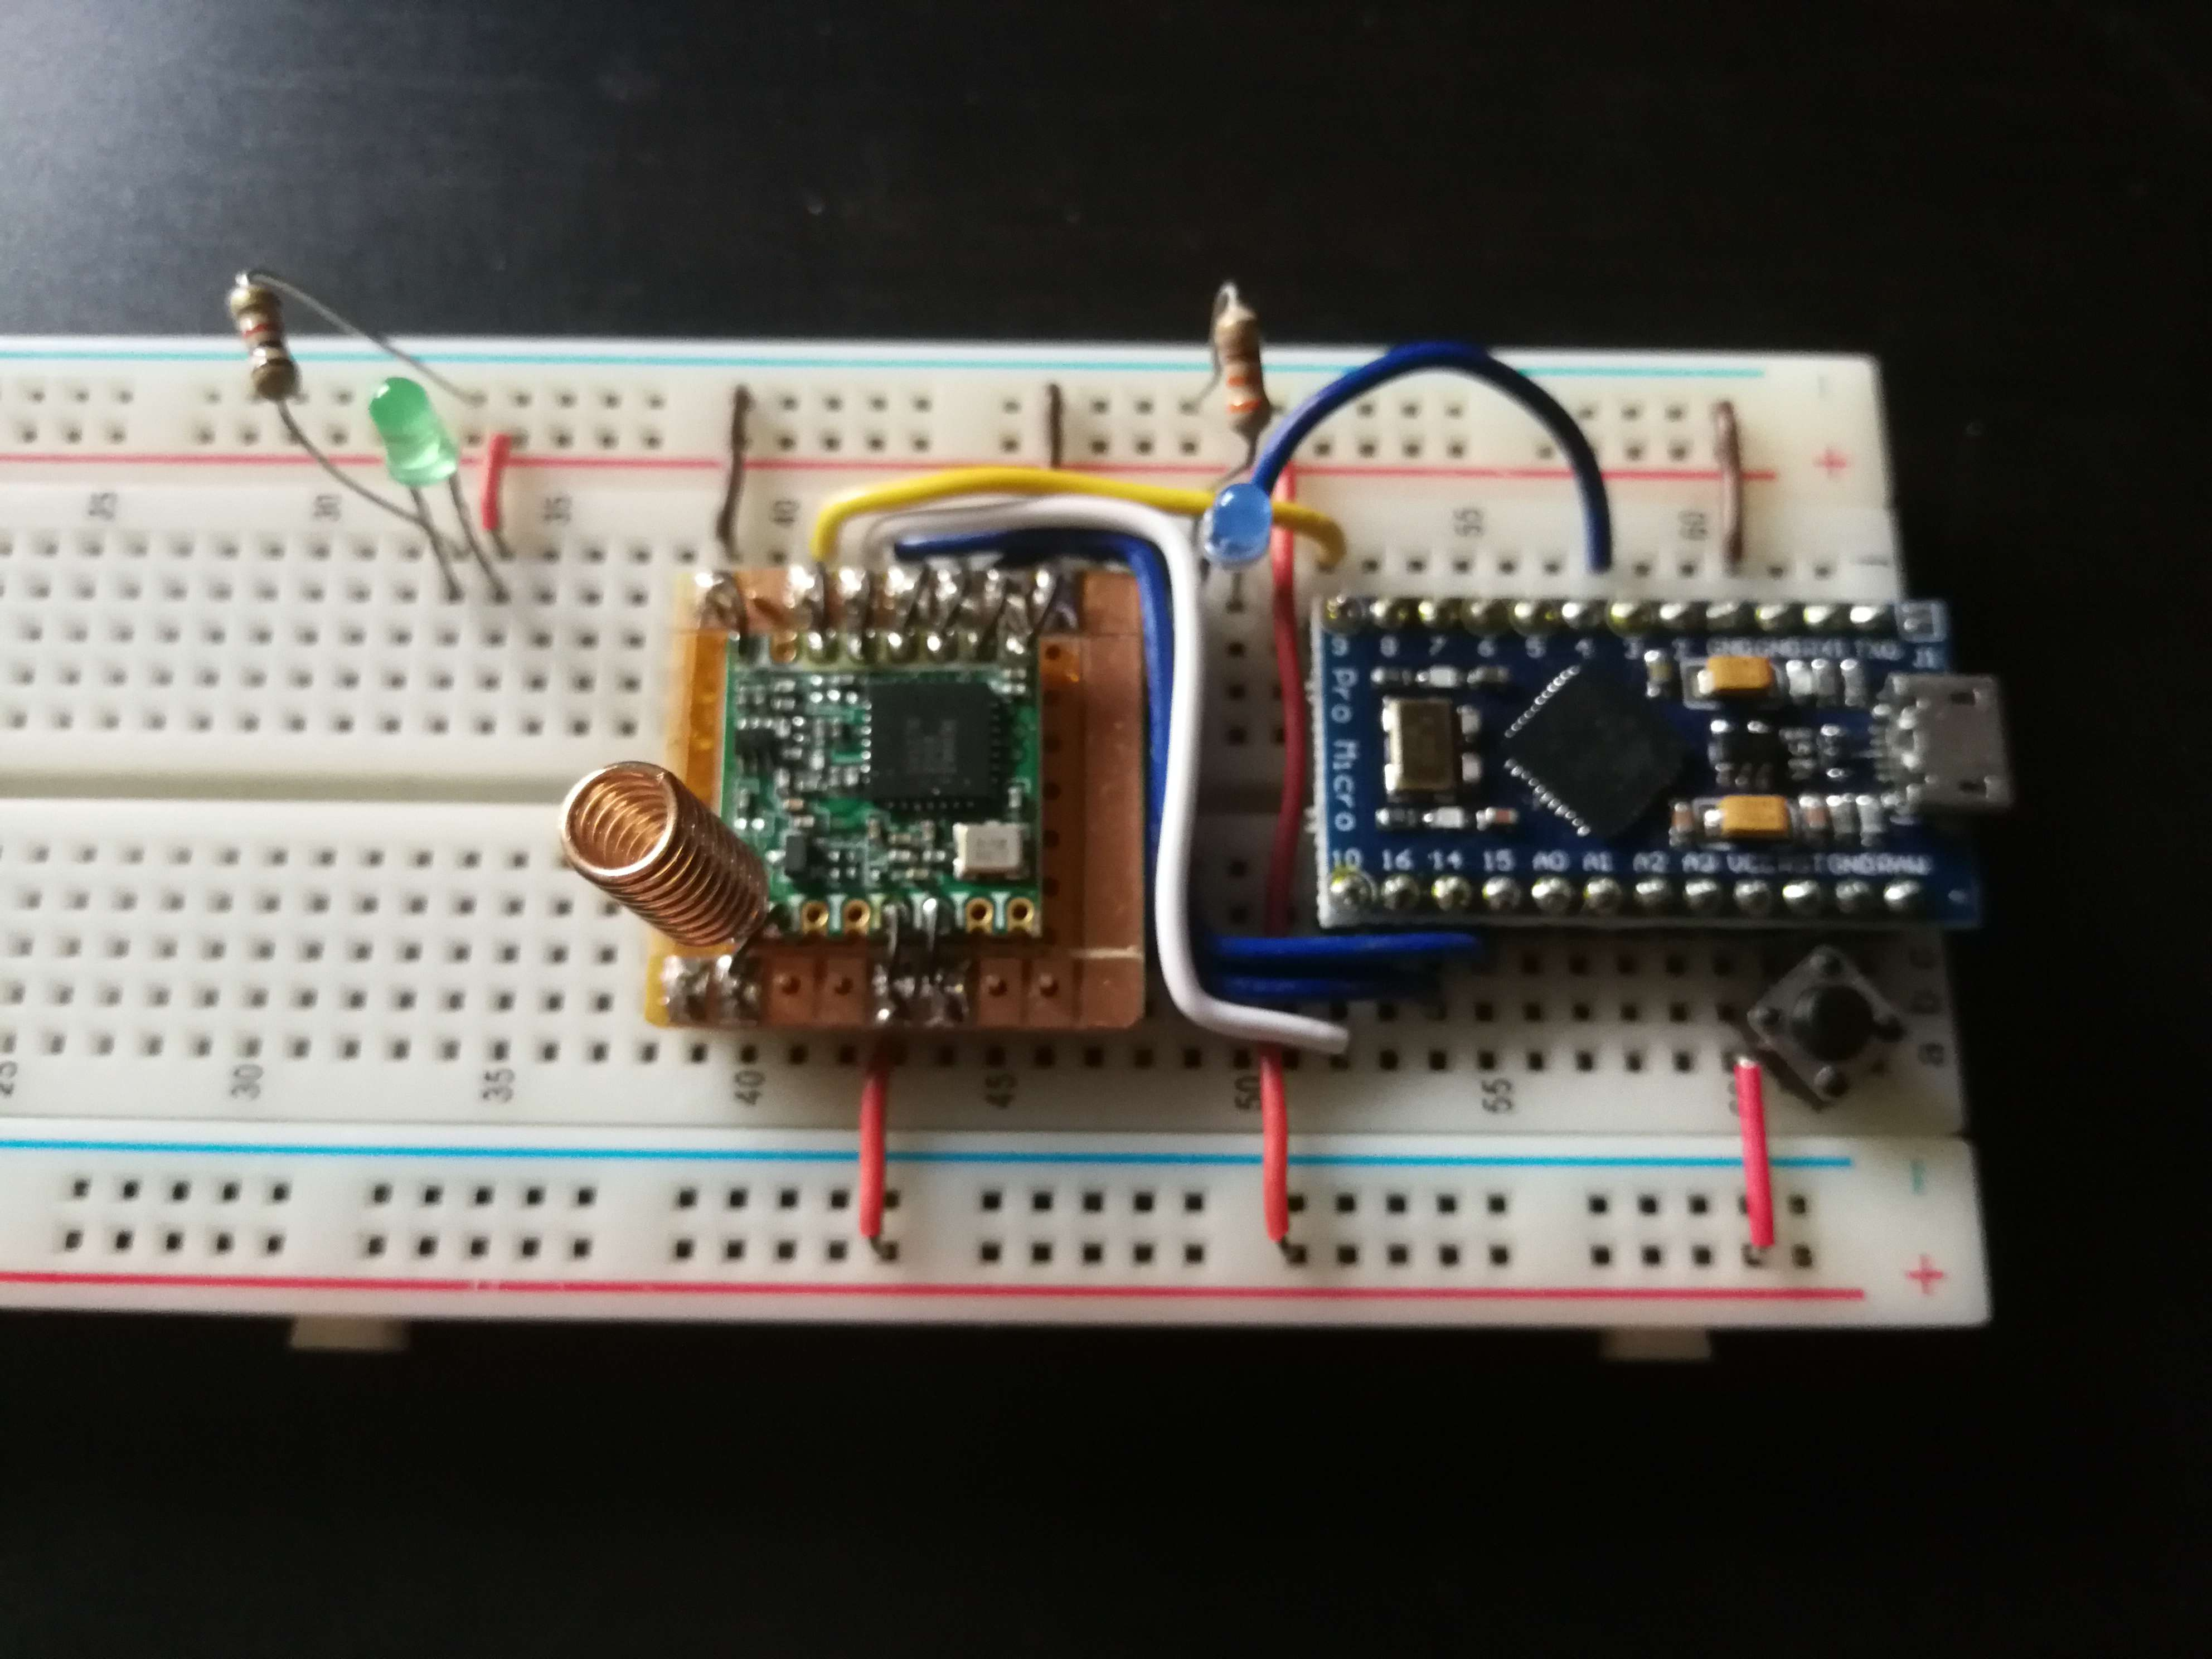
\includegraphics[scale=0.07]{images/arduino.png}
\caption{Un module Arduino}\label{term36}
\end{figure}

L'avantage principal du module \textit{Arduino} est qu'il est possible de configurer une largeur de bande bien plus faible que les autres modules. Les modules RN2483 ou LoPy ont une largeur de bande minimale de 125KHz, tandis qu'avec l'arduino il est possible de descendre jusqu'à 7.8 KHz. Il est également possible de réduire le facteur d'étalement en dessous de la valeur imposée par LoRa (minimum de LoRa SF = 7, ici SF = 6 possible). Pour rappel, une largeur de bande plus faible permet un \textit{time on air (TOA)} plus grand, ce qui est très utile pour analyser les signaux. Le transceiver est de type SX127x (comme celui du RN2483).

\vspace{0.1cm}

L'utilisation de l'IDE Arduino 2.2.1 est nécessaire pour la configuration du module Arduino décrit dans la section \ref{arduino}. L'IDE permet d'uploader le code  dans le module. Le code est disponible dans l'annexe \ref{codearduino}.

\subsection{Logiciels}\label{fft}

Une fois les différents appareils choisis, il faut les accompagner avec les softwares adéquats. Ainsi il faut des logiciels d'analyse de signaux compatibles avec les différents modules et radios logicielles.

\subsubsection{GQRX}

Le premier logiciel choisi est \textit{GQRX}. c'est un logiciel open source d'analyse de fréquences radio pour les SDR. Le fonctionnement du logiciel est assez direct, la figure \ref{term37} montre comment configurer simplement le logiciel.

\begin{figure}[h]
\centering
\begin{subfigure}{0.4\textwidth}
  \centering
  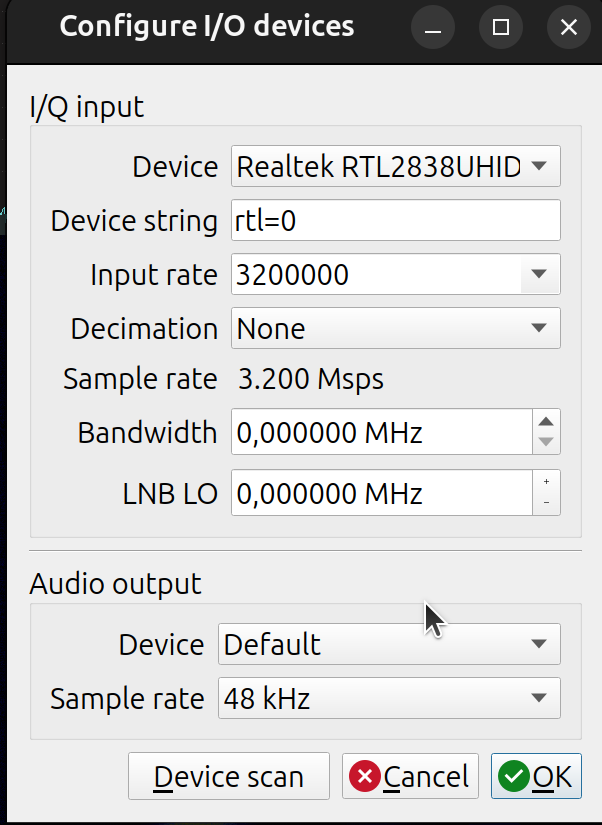
\includegraphics[width=\textwidth]{images/gqrx2.png}
  \caption{SDR input}
  \label{term331}
\end{subfigure}
\hspace{0.5cm} % Adjust the horizontal space between the subfigures
\begin{subfigure}{0.4\textwidth}
  \centering
  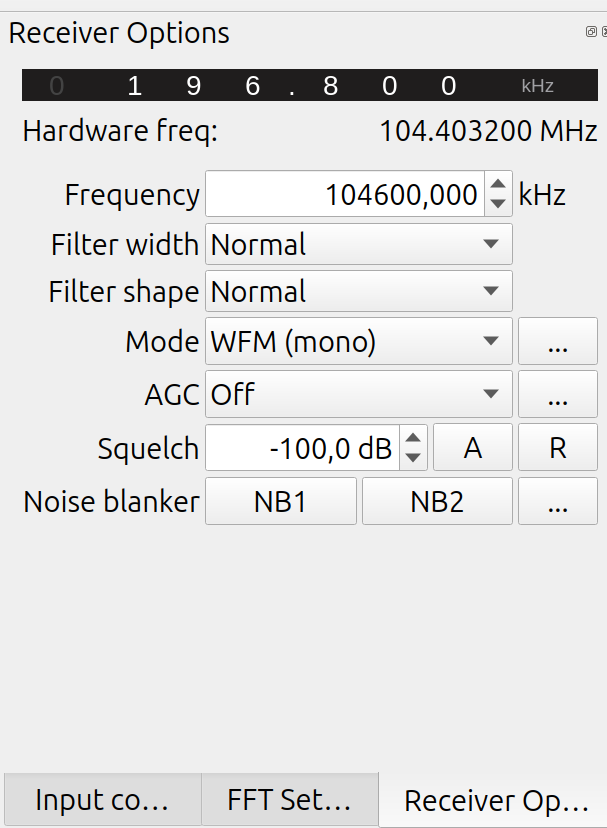
\includegraphics[width=\textwidth]{images/gqrx3.png}
  \caption{Receiver options}
  \label{term341}
\end{subfigure}
\caption{Configuration de GQRX}
\label{term37}
\end{figure}

La figure \ref{term331} demande de compléter les paramètres suivants:

\vspace{0.1cm}

\begin{itemize}
\item \textbf{Device}: il faut sélectionner la SDR dans la liste des appareils. Le \textit{Device String} fait référence à cet appareil dans GQRX.
\item \textbf{Input rate}: le taux d'échantillonage capturé par la SDR, il apparait plus bas comme \textit{sample rate}.
\item \textbf{Decimation}: c'est un procédé qui permet de réduire le nombre d'échan\-tillons gérés par le logiciel, pour économiser des ressources.
\item \textbf{Bandwidth}: la largeur de bande supplémentaire que peut gérer la SDR.
\item \textit{Low Noise Block Local Oscillator (\textbf{LNB LO})}: ce paramètre est spécifique à la réception satéllite et représénte le frequency offset aplliqué par l'oscillateur locale dans un LNB downconverter.
\item L'\textbf{Audio output} concerne la sortie sonore du signal.
\end{itemize}

\vspace{0.1cm}

La figure \ref{term341} ajoute des paramètres pour le récepteur, c'est à dire pour l'interface de GQRX :

\vspace{0.1cm}

\begin{itemize}
\item \textbf{frequency}: la fréquence que l'on souhaite écouter.
\item \textbf{Filter Width}: ce paramètre permet de changer la taille de la largeur de bande du filtre appliqué au signal.
\item \textbf{Filter Shape}: contrairement au Filter Width ce n'est pas la taille mais la forme du filtre que l'on peut modifier.
\item \textbf{Mode}: le mode de démodulation.
\item \textbf{Automatic Gain Control (ACG)}: l'ACG ajuste le gain du récepteur pour maintenir un signal constant.
\item \textbf{Squelch}: c'est un threshold qui coupe la sortie sonore s'il est franchi.
\item \textbf{Noise blanker}: c'est une fonctionnalité qui permet de réduire l'impact des interférences sur le signal.
\end{itemize}

\vspace{0.1cm}

La figure \ref{term38} montre un exemple de ce qu'on observe quand on écoute la fréquence radio de Classic21. GQRX affiche le signal reçu sous deux formes différentes : en spectre et en cascade.

\vspace{0.1cm}

L'affichage du spectre fournit une représentation graphique en temps réel du spectre RF sur une gamme de fréquences.
Il montre la puissance du signal de différentes fréquences sur une plage de fréquences spécifiée.
L'axe horizontal représente la fréquence, tandis que l'axe vertical affiche la force du signal (mesurée en dB).

\vspace{0.1cm}

L'affichage en cascade est un spectrogramme qui visualise la force du signal au fil du temps.
Il montre une série de spectres instantannés empilés les uns sur les autres, où l'intensité de la couleur représente la force du signal.
Chaque ligne horizontale du tracé en cascade représente une vue du spectre capturée à un moment précis, créant ainsi un enregistrement de l'activité du signal.
L'axe horizontal représente la fréquence et l'axe vertical représente le temps.

\newpage

\begin{figure}[h]
\centering

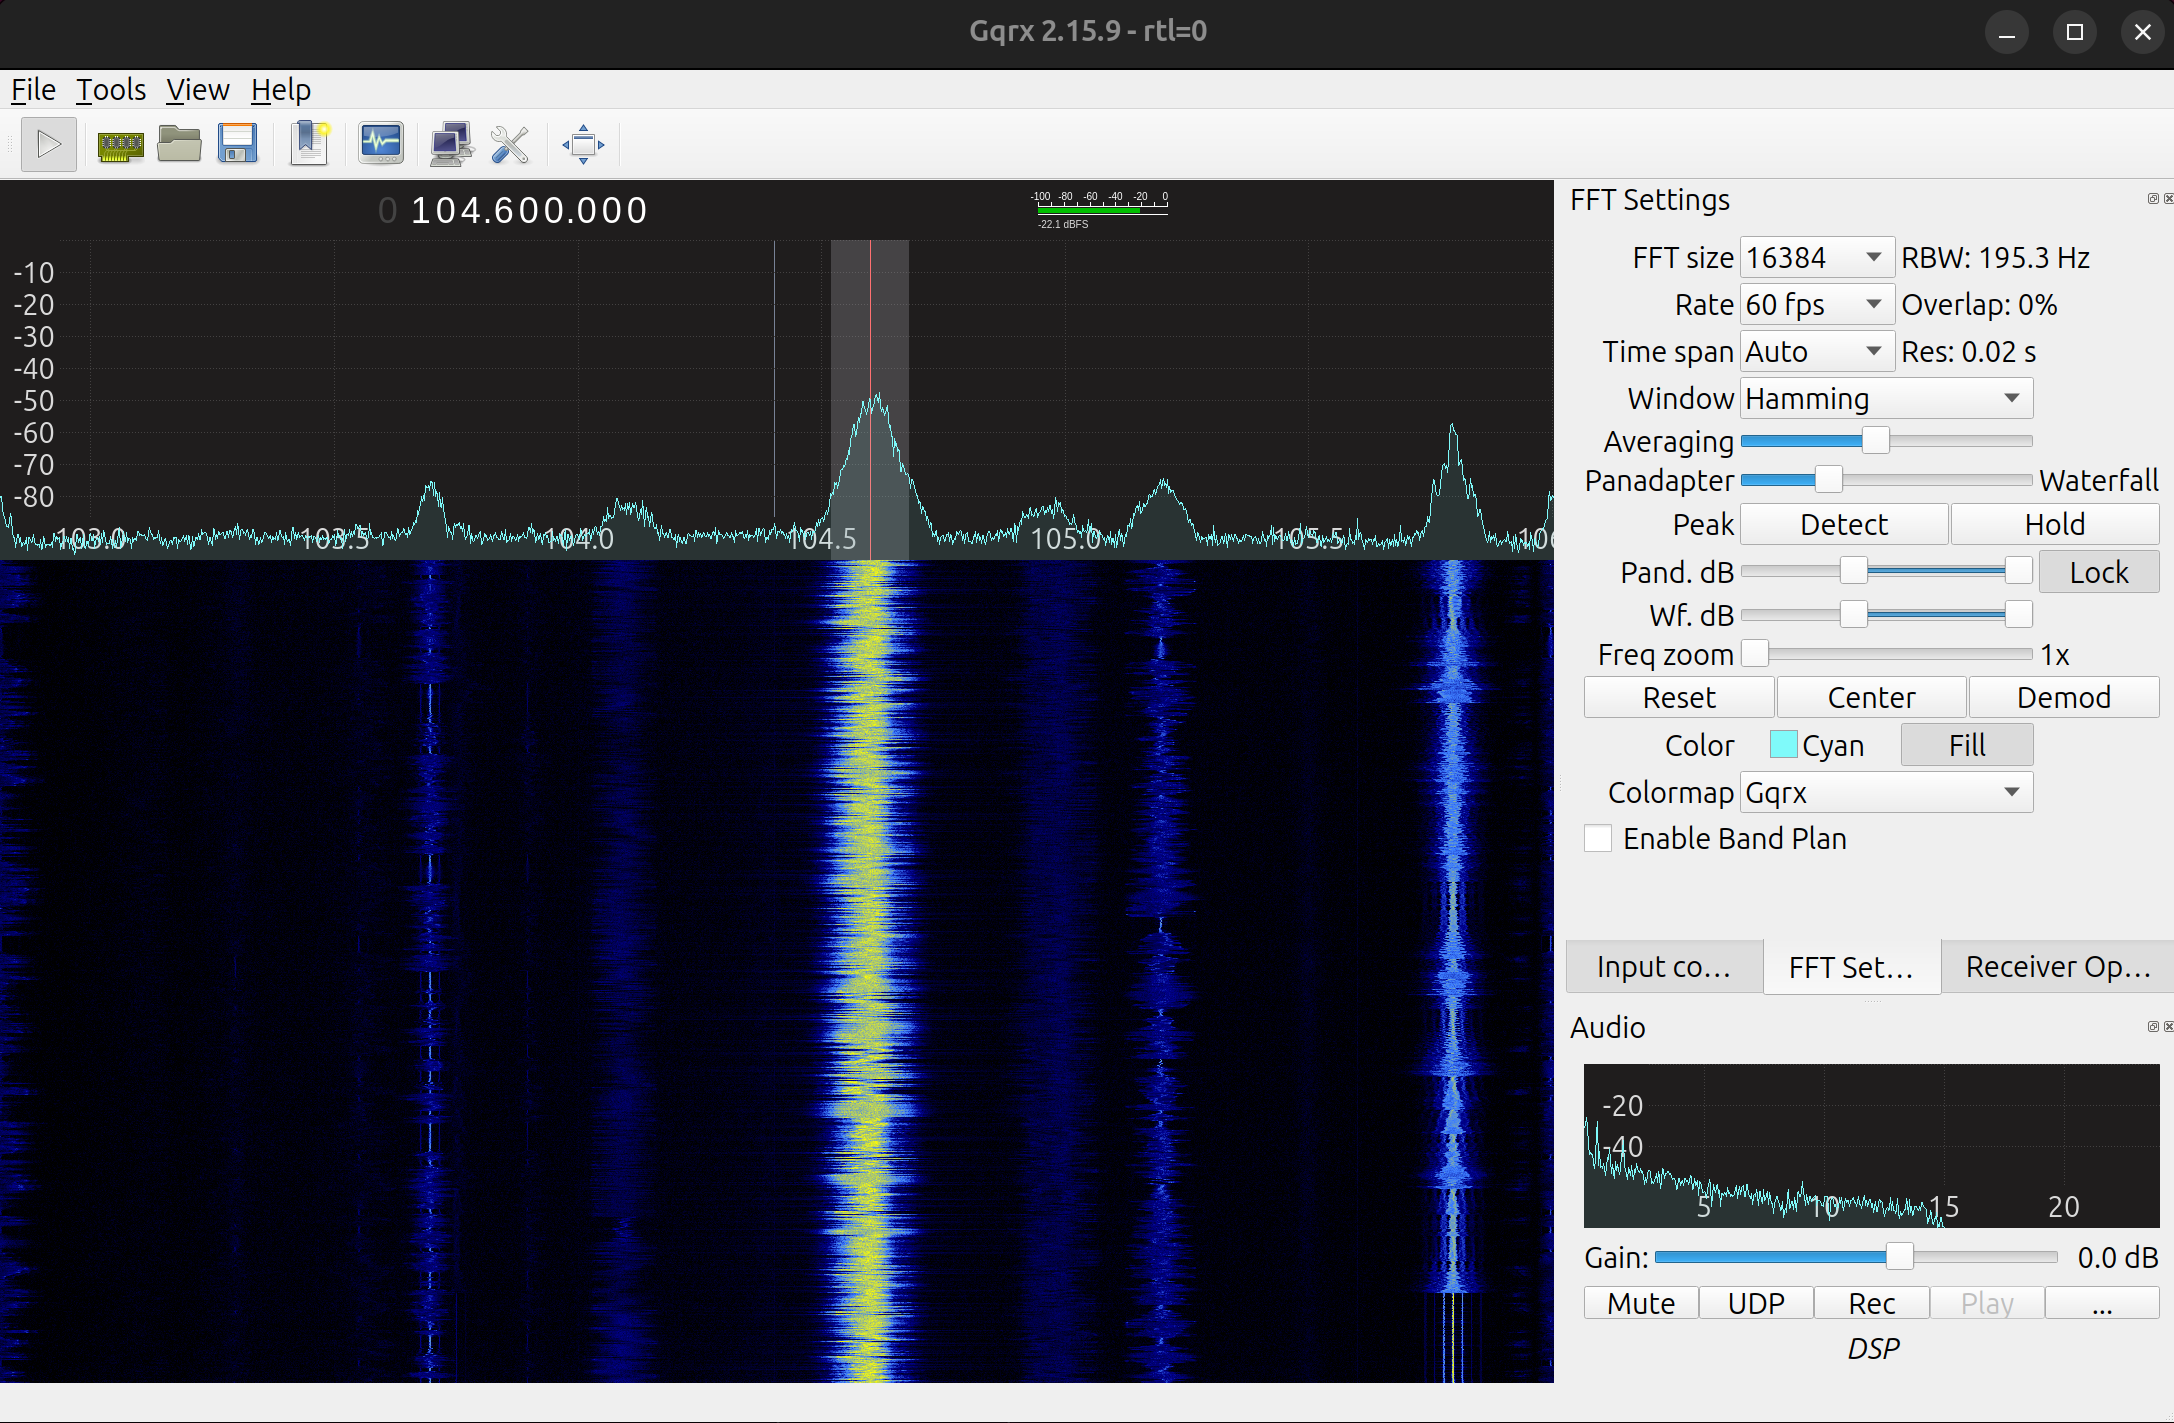
\includegraphics[scale=0.18]{images/gqrx1.png}
\caption{Réception de la station radio Classic21}\label{term38}
\end{figure}

Durant la réception du signal, il est possible de modifier l'affichage. A droite de l'affichage en spectre et en cascade sur la figure \ref{term38}, il y a différents paramètres :

Pour l'affichage en spectre, le paramètre \textbf{Panadapter dB} représente la force du signal des fréquences radio reçues affichées sur l'axe vertical du graphique du spectre. Pour l'affichage en cascade, le paramètre \textbf{Waterfall dB} modifie l'intensité utilisée pour afficher la force du signal, permettant ainsi d'ajuster le contraste ou la visibilité des signaux plus faibles ou plus forts. 

\vspace{0.1cm}

Les paramètres suivants sont communs et affectent les deux affichages :

\vspace{0.1cm}

Le paramètre \textbf{FFT size} détermine le nombre d'échantillons utilisés dans chaque calcul de la FFT. Une valeur plus large donne un meilleure résolution, mais consomme plus de ressources. La valeur est une puissance de deux pour des raisons d'éfficacité de calculs.

\vspace{0.1cm}

Le paramètre \textbf{Rate} détermine le taux de rafraichissement de l'affichage. Un taux relativement faible avec une taille de frame FFT élevé induit un effet d'overlap, c'est à dire que des frames consécutives partagent des échantillons, ce qui donne un affichage plus lisse du spectre.


\subsubsection{Universal radio hacker, URH}


Universal Radio Hacker est un logiciel open source similaire à GQRX. Son role principal est l'analyse de signaux radio. Au dela de l'écoute en temps réel, URH peut sauvegarder des signaux et lire des enregistrements à partir de fichiers. La figure \ref{term39} montre comment enregistrer un signal. Les paramètres à configurer sont similaires à GQRX (le choix de la SDR, le fréquence, le taux d'échantillonage, la largeur de bande et le gain). Comme URH est le principal outil d'analyse pour ce travail, les analyses avec ce dernier sont détaillées dans la section \ref{urh}.

\begin{figure}[h]
\centering

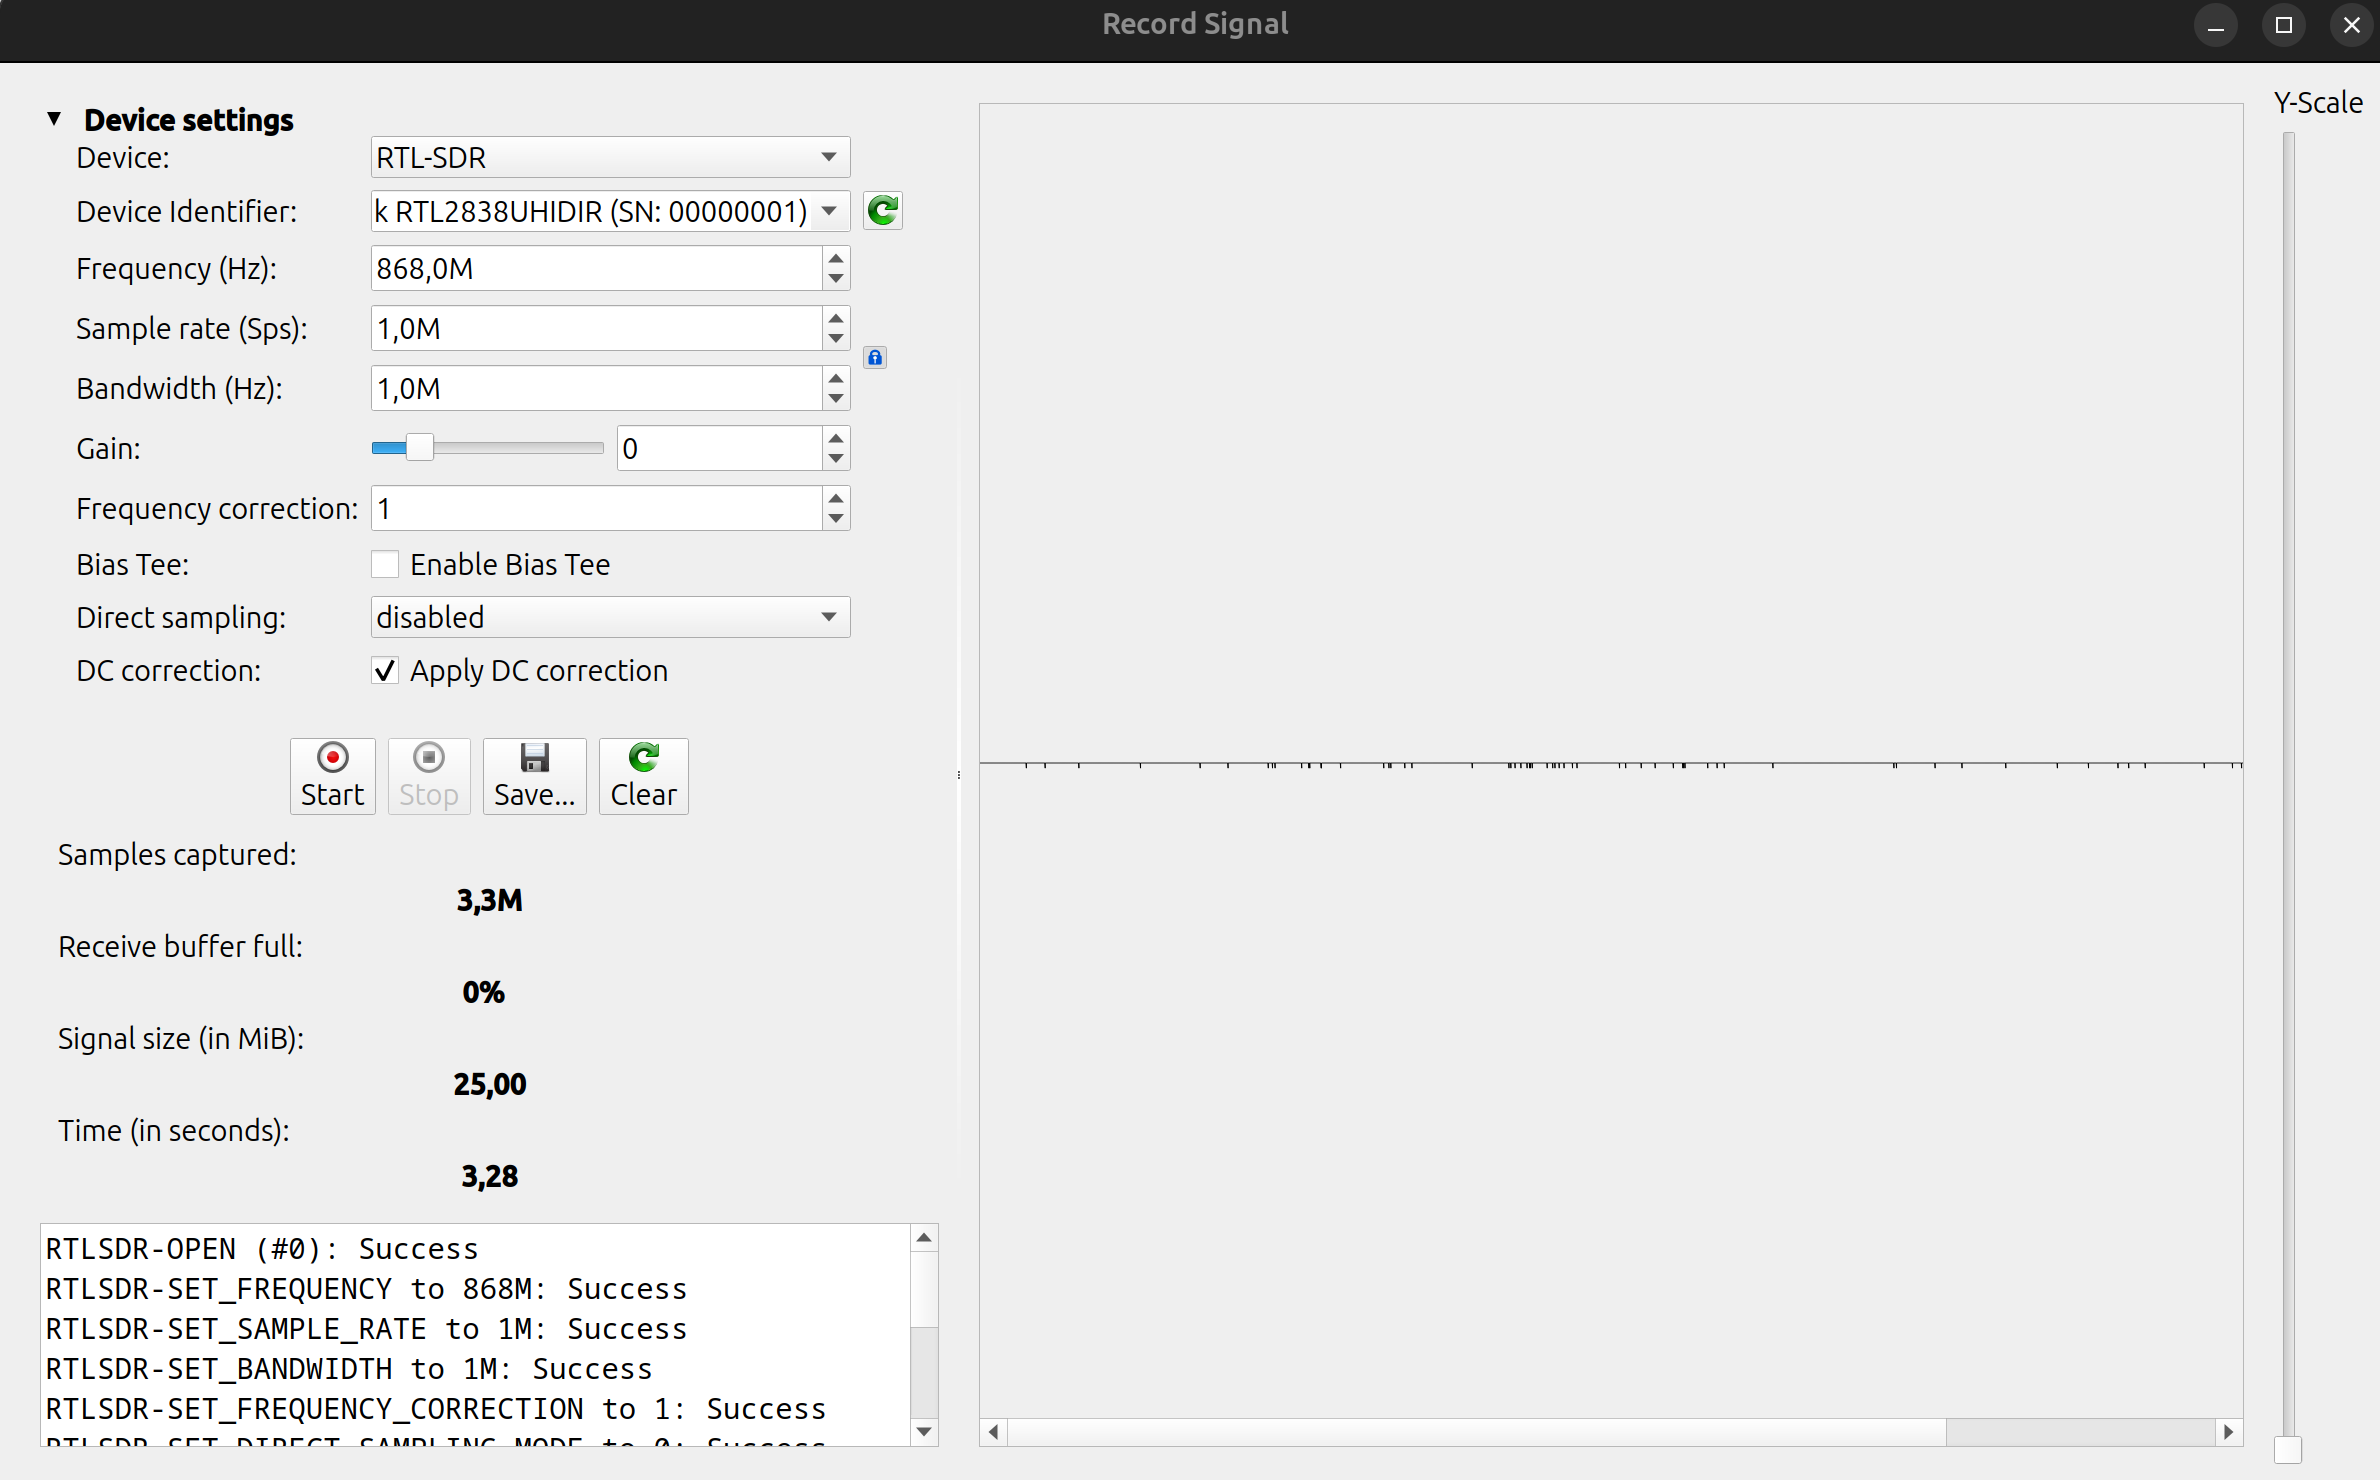
\includegraphics[scale=0.16]{images/urh1.png}
\caption{Enregistrement d'un signal avec URH}\label{term39}
\end{figure}

\newpage

Les fichiers qu'URH peut interpréter ou enregistrer sont au format \textit{.complex}. Ce format est utilisé pour sauvegarder les signaux sous forme d'échantillons \textit{I/Q (In phase / Quadrature)} Il existe plusieurs variantes de ce format supporté par URH :

\vspace{0.1cm}

\begin{table}[h]
\centering
\begin{tabular}{|c|c|c|c|}
\hline
\multicolumn{1}{|c|}{} & \multicolumn{1}{c|}{Taille I (bits)} &\multicolumn{1}{c|}{Taille Q (bits)} & \multicolumn{1}{c|}{Type}\\
\hline
.complex & 32 & 32 & float \\
\hline
.complex64 & 32 & 32 & float\\
\hline
.complex16u & 8 & 8 & unsigned int\\
\hline
.complex16s &  8 & 8 & int\\
\hline
.complex32u & 16 & 16 & unsigned int \\
\hline
.complex32s & 16 & 16 & int  \\
\hline
\end{tabular}
\caption{Table des formats supportés par URH}
\label{format}
\end{table}



\section{Python}

Le choix du langage pour l'implémentation du travail est Python (version 3.11.4). Python donne l'accès à plusieurs librairies très pertinentes pour faire du \textit{signal processing}. Voici les principales librairies utilisées :

\vspace{0.1cm}

\begin{itemize}
\item \textit{Numpy}. Cette librairie est fondamentale pour la gestion des \textit{arrays}. Elle contient également de nombreuses fonctions et formats mathématiques utiles au projet.
\item \textit{Matplotlib}. Cette librairie permet d'effectuer des plots des données de manière simple et efficace.
\item \textit{PyRTLSDR}. La librairie PyRTLSDR est essentielle pour pouvoir manipuler la SDR R820T2. Il est possible de configurer la SDR sans devoir passer par un software tier comme GQRX ou URH grâce à cette librairie.
\item \textit{PyHackRf}. L'équivalent de PyRTLSDR mais pour la SDR HackrF One.
\item \textit{Datashader}. Cette librairie permet la visualisation améliorée de grande quantité de données via l'ajout de gradient coloré.
\item \textit{Serial}. La manipulation des modules rn2483 est possible grave à la librairie serial. Cette librairie permet d'intéragir avec les apparails connecté via USB.
\end{itemize}

\newpage

L'environement de travail utilisé est Visual Studio Code (version 1.87.1). Cet IDE est open source et largement populaire ce qui permet un apprentissage pour des travaux spécifiques très rapides via Internet. L'utilisation de VSCode est motivée par son système d'extension, qui contient plusieurs extensions qui permettent de manipuler directement les modules d'émission LoRa. Le module Lopy de Pycom est compatible avec VSCode via l'extension PyMakr. GitHub est également intégré dans VSCode, ce qui permet de simplifier la mise en ligne du travail.

\begin{table}[h]
\centering
\begin{tabular}{|p{4cm}|p{2cm}|p{2cm}|p{3.5cm}|}
\hline
\multicolumn{1}{|c|}{Caractéristiques importantes} & \multicolumn{1}{c|}{GQRX} & \multicolumn{1}{c|}{URH} & \multicolumn{1}{c|}{Python}\\
\hline
Interface Utilisateur & GUI avec affichage en temps réel & GUI avec outils plus poussés pour analyse & / \\
\hline
Réception de signaux & \multicolumn{3}{c|}{oui} \\
\hline
Génération de signaux & non & \multicolumn{2}{c|}{oui} \\
\hline
Sauvegarde des données & pas de sauvegarde possible & \multicolumn{2}{c|}{sauvegarde et chargement possibles} \\
\hline
Format des données & / & voir table \ref{format} & .complex64 jusqu'à .complex512 \\
\hline
Démodulation &  &  & toutes\\
\hline
Courbe d'apprentissage & prise en main très rapide & prise en main rapide & plus de possibilités donc plus de temps d'apprentissage \\
\hline
Analyse du signal & concentrée sur le temps réel & \multicolumn{2}{c|}{concentrée sur l'analyse en profondeur} \\
\hline
SDR supportées & \multicolumn{3}{c|}{toutes les SDR présentées} \\
\hline
\end{tabular}
\caption{Table comparative des logiciels utilisés}
\label{table2}
\end{table}

GQRX offre globalement de meilleurs outils pour la visualisation en temps réel, là où URH permet l'analyse de manière plus précise et avec plus de possibilités. Python permet une customisation encore plus poussée à condition de manuellement rajouter ces fonctionnalités.

\newpage

\section{Géneration et réception d'un signal LoRa} \label{signallora}

La première étape de l'expérimenation consiste à générer via un module un signal LoRa et à le capturer à l'aide d'une radio logicielle. Pour cette première étape, le module d'émission choisi est le module RN2483, car il est le plus facile et rapide à configurer.
Via python, il est possible d'utiliser la librairie \textit{Serial} pour se connecter au port usb reliant le module à l'ordinateur. Ensuite, via les différentes commandes, on configure le module en modifiant les paramètres suivants : 

\vspace{0.1cm}

\begin{itemize}
\item la modulation, en LoRa.
\item La fréquence. 868MHz, la fréquence de la bande ISM , la bande d'émission en Europe.
\item La largeur de bande choisie est de 125Khz, ce qui est la plus petite valeur possible que permet le module.
\item La puissance du module, au maximum (14dBm).
\item Le spreading factor, la valeur la plus grande possible est choisie (SF = 12).
\item Le coding rate. Il y a 4 valeur possibles: 4/5, 4/6, 4/7 and 4/8. Cela signifie que tout les 4 bits seront codé par 4, 5, 6, 7 ou 8 bits de transmissions en fonction de cette valeur. Plus la valeur est faible (la plus faible étant 4/8), plus le TOA sera élevé, car cela prend plus de temps pour transmettre le message.
\item Le message à envoyer. Le but de cette expérimentation n'est pas de récupérer l'information initiale (le contenu du message), il n'a donc pas un grand intérêt. Le message à envoyer est un nombre héxadécimal : $0x1509ACF$.
\end{itemize}

\vspace{0.1cm}

Le choix des valeurs pour les différents paramètres est de maximiser le TOA. Les commandes relatives à la configuration sont disponibles dans l'annexe \ref{codern}

\subsection{Analyse avec GQRX}

Une fois que le module est configuré, il faut paramètrer le recepteur, la radio logicielle. La SDR choisie est la RTL SDR T820R2. Voici les paramètres de la SDR:

\vspace{0.1cm}

\begin{itemize}
\item la fréquence. La fréquece d'écoute, idéalement la même fréquence de celle de l'émetteur (868MHz).
\item Le taux d'échantillonage. Il est possible de choisir la quantité d'échantillons traitée chaque seconde. Un taux plus élevé donnera un signal plus complet. Le taux minimal ne doit jamais être inférieur à deux fois la largeur de bande (Théorème de Nyquist-Shannon).
\item Le gain. Dépendant de la qualité du signal il peut être nécessaire d'ajouter du gain, c'est à dire d'amplifier la force du signal. Un gain trop élevé peut saturer le signal, c'est à dire quand l'amplitude dépasse la portée du récepteur.
\end{itemize}

\vspace{0.1cm}

La figure \ref{term301} montre la capture de deux signaux LoRa. On remarque que malgré la configuration des paramètres pour maximier le TOA, il est difficile d'observer en détail le signal. On observe également que le signal se situe entre la fréquence 867,915MHz et 868,040MHz, ce qui correspond bien à la largeur de bande de 125Khz (0.125MHz) choisie.

\begin{figure}[h]
\centering

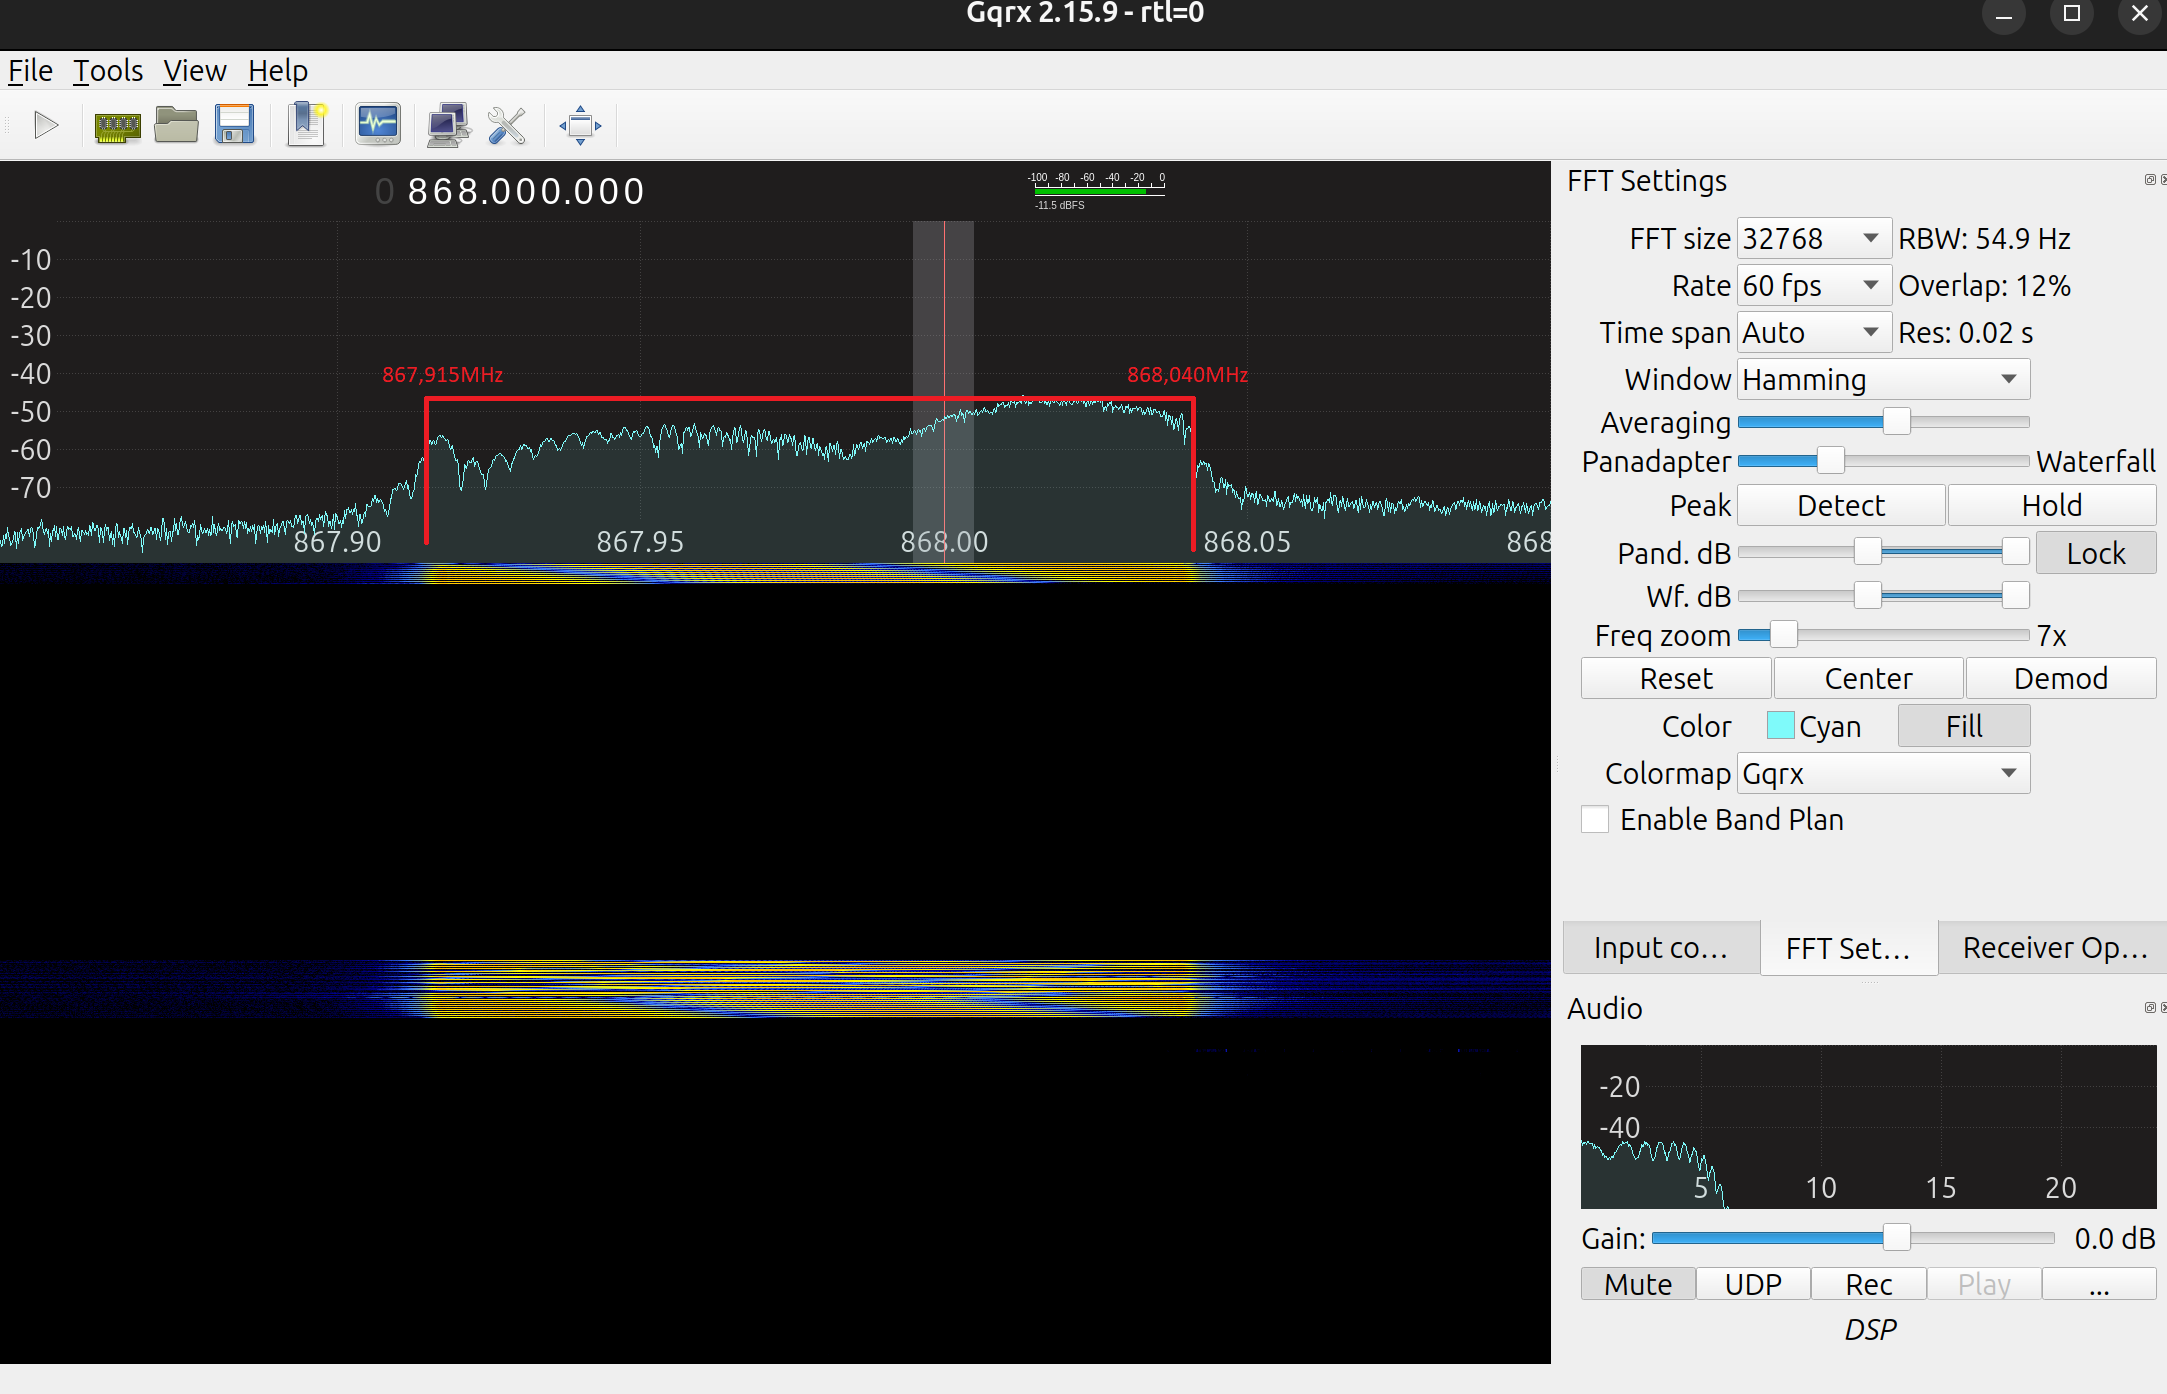
\includegraphics[scale=0.28]{images/gqrx4.png}
\caption{capture module rn2483 sur GQRX avec RTLSDR R820T2. Sample rate = 1.8MHz}\label{term301}
\end{figure}

Le module Arduino, contrairement aux modules Pycom et RN2483, permets d'utiliser une largeur de bande beaucoup plus faible. La figure \ref{term302} montre la capture d'un signal LoRa émis depuis le module Arduino. La largeur de bande choisie est de 7.8Khz, les autres paramètres d'émissions (la modulation, la fréquence et le spreading factor) sont similaires à ceux de la capture précédente. Cette fois ci, on distingue clairement sur l'affichage en spectre un pic à 868,070MHz. Sur l'affichage en cascade, le signal se dessine sous forme de traits (les chirps). Cela correspond bien à la théorie de la modulation LoRa où le signal modulé est composé de upchirps et downchirps. Il y a de part et d'autre du signals des silhouettes. Cela est dû à la sensibilité de la SDR, si on observe les pics de fréquences dans l'affichage en spectre, on constate qu'ils sont négligeables car leurs échelles de puissances sont bien inférieures (environ 60dB plus faible) à celle du pic principal. GQRX permet de visualiser le signal, mais pour pousser l'analyse plus en détails d'utilisation d'Universal Radio Hacker est nécessaire.

\begin{figure}[h]
\centering

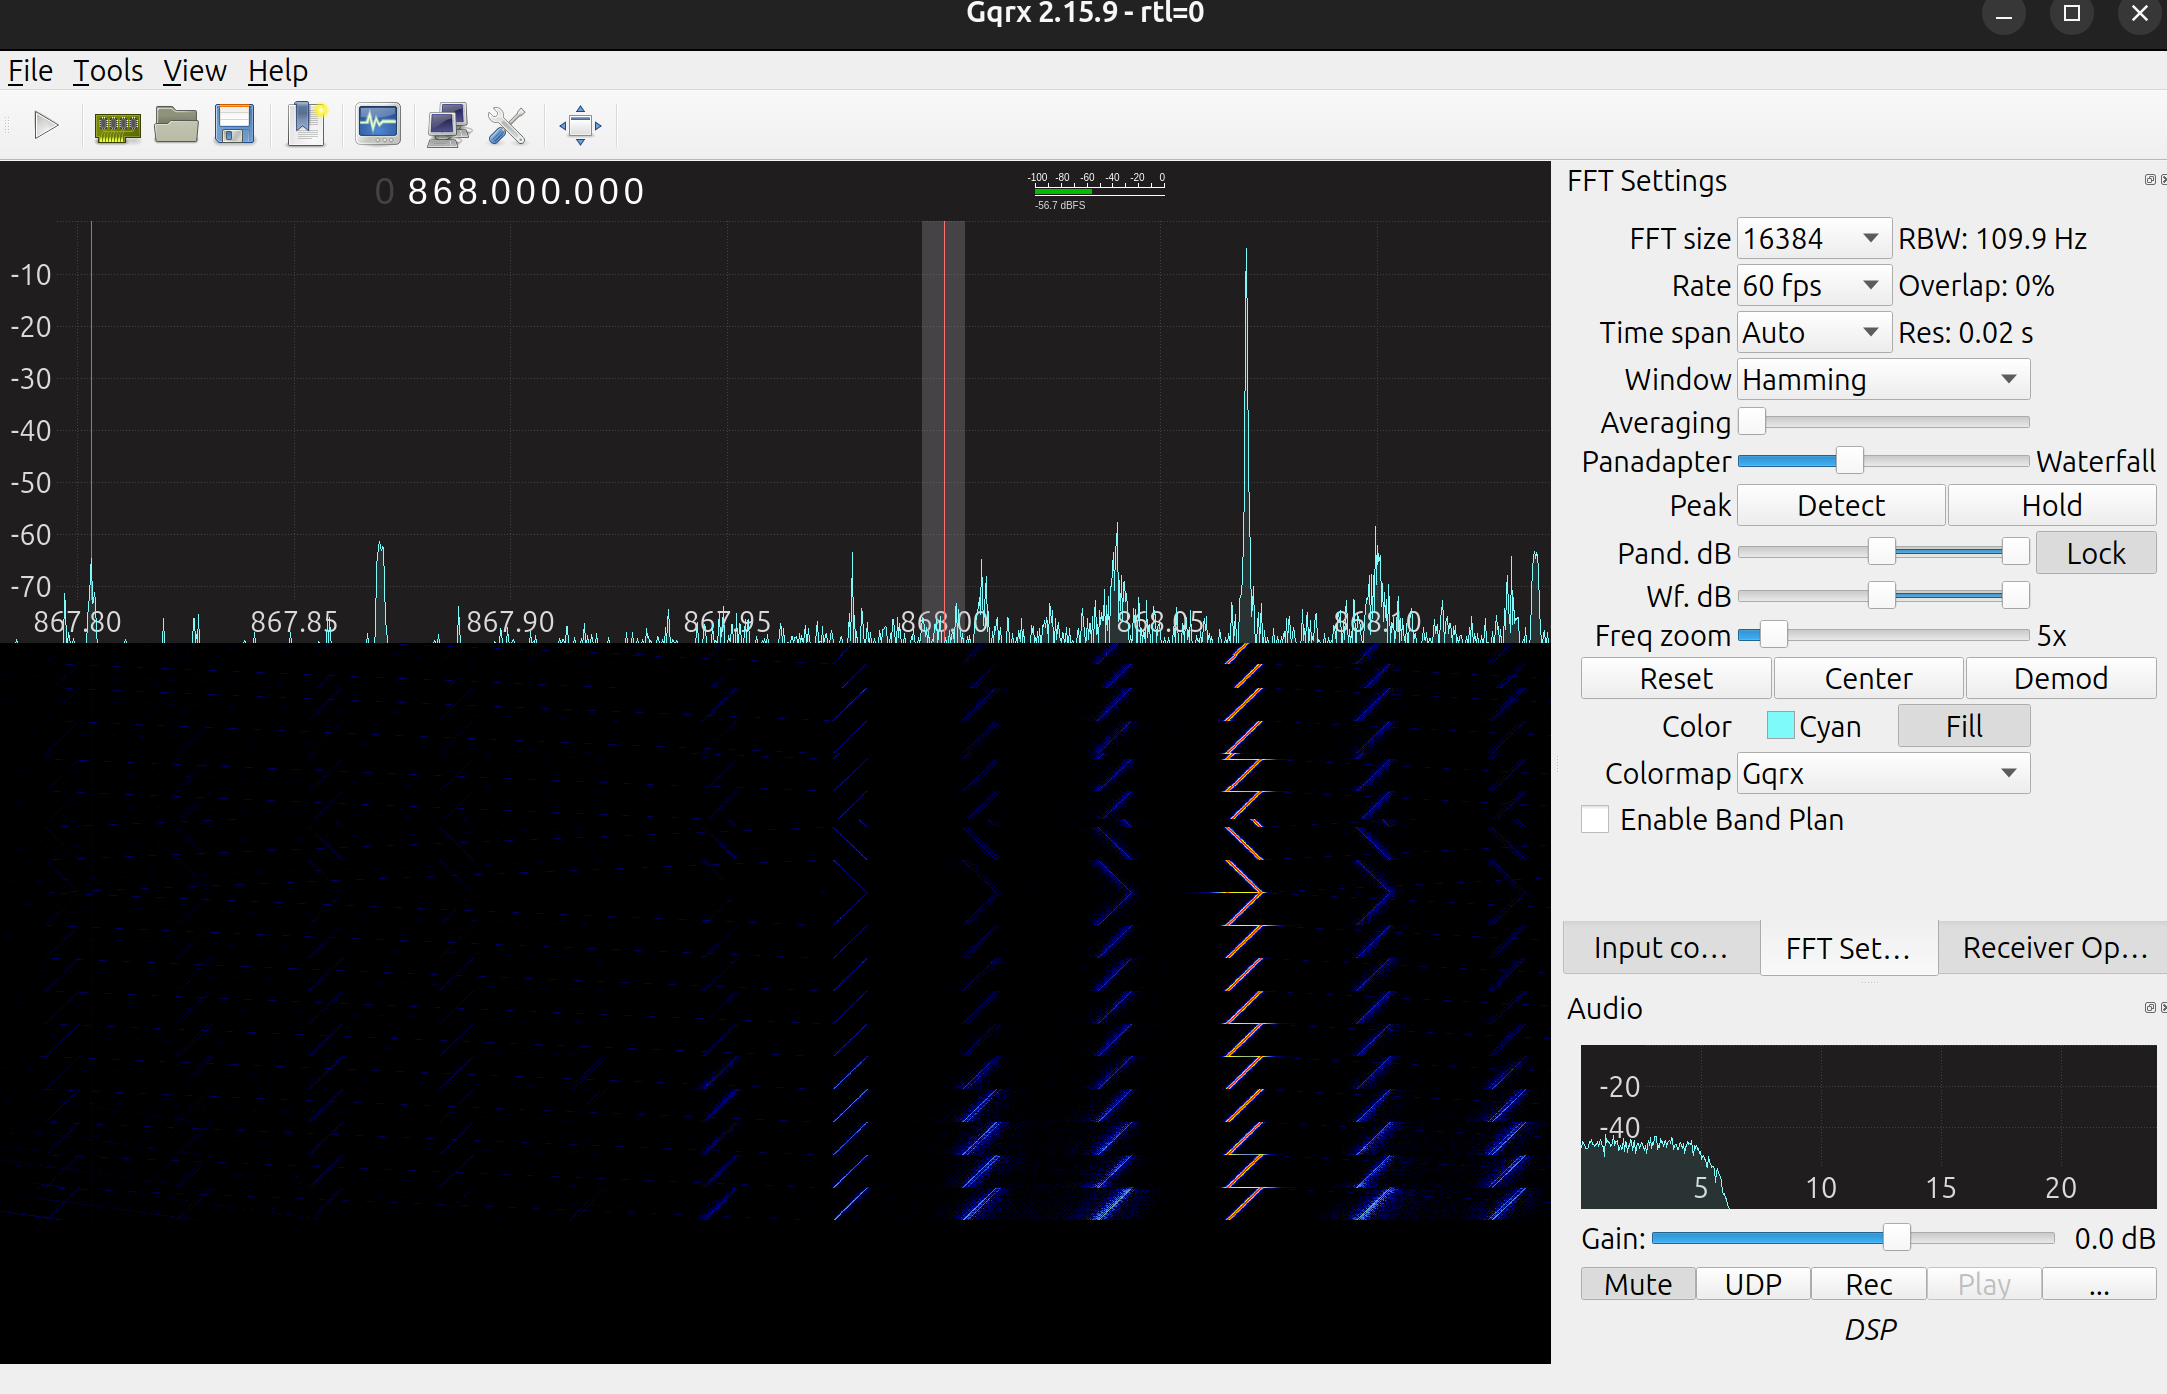
\includegraphics[scale=0.17]{images/gqrx5.png}
\caption{capture module Arduino sur GQRX avec RTLSDR R820T2 Sample rate = 1.8MHz}\label{term302}
\end{figure}


\subsection{Analyse avec URH}\label{urh}

GQRX permet de zoomer sur les fréquences mais pas sur le temps, ce qui demande donc de générer un signal dont le TOA doit être le plus élevé possible. URH offre plus de flexibilité sur l'analyse ce qui permet de ne pas devoir utiliser des largeurs de bande aussi faibles que celles du module Arduino. Ainsi, pour l'analyse avec URH, les modules Pycom et RN2483 sont utilisés. La figure \ref{term303} et \ref{term304} montre la capture et la sauvegarde d'un signal LoRa. Le module utilisé est rn2483, la SDR est la R820T2. les paramètres d'émission sont les suivants : BW = 125KHz, SF = 8, freq = 868MHz, Mode = LoRa, cr = 4/8, pwr = 14. Les paramètres du récepteurs sont les suivants : frequency = 868MHz, SR = 1.8MHz, gain = 0dB. Pour des raisons de sipmlicité, le signal capturé avec ses paramètres sera utilisé comme référence pour toute la partie analyse jusqu'à la fin de la section \ref{signallora}.

\newpage

\begin{figure}[h]
\centering

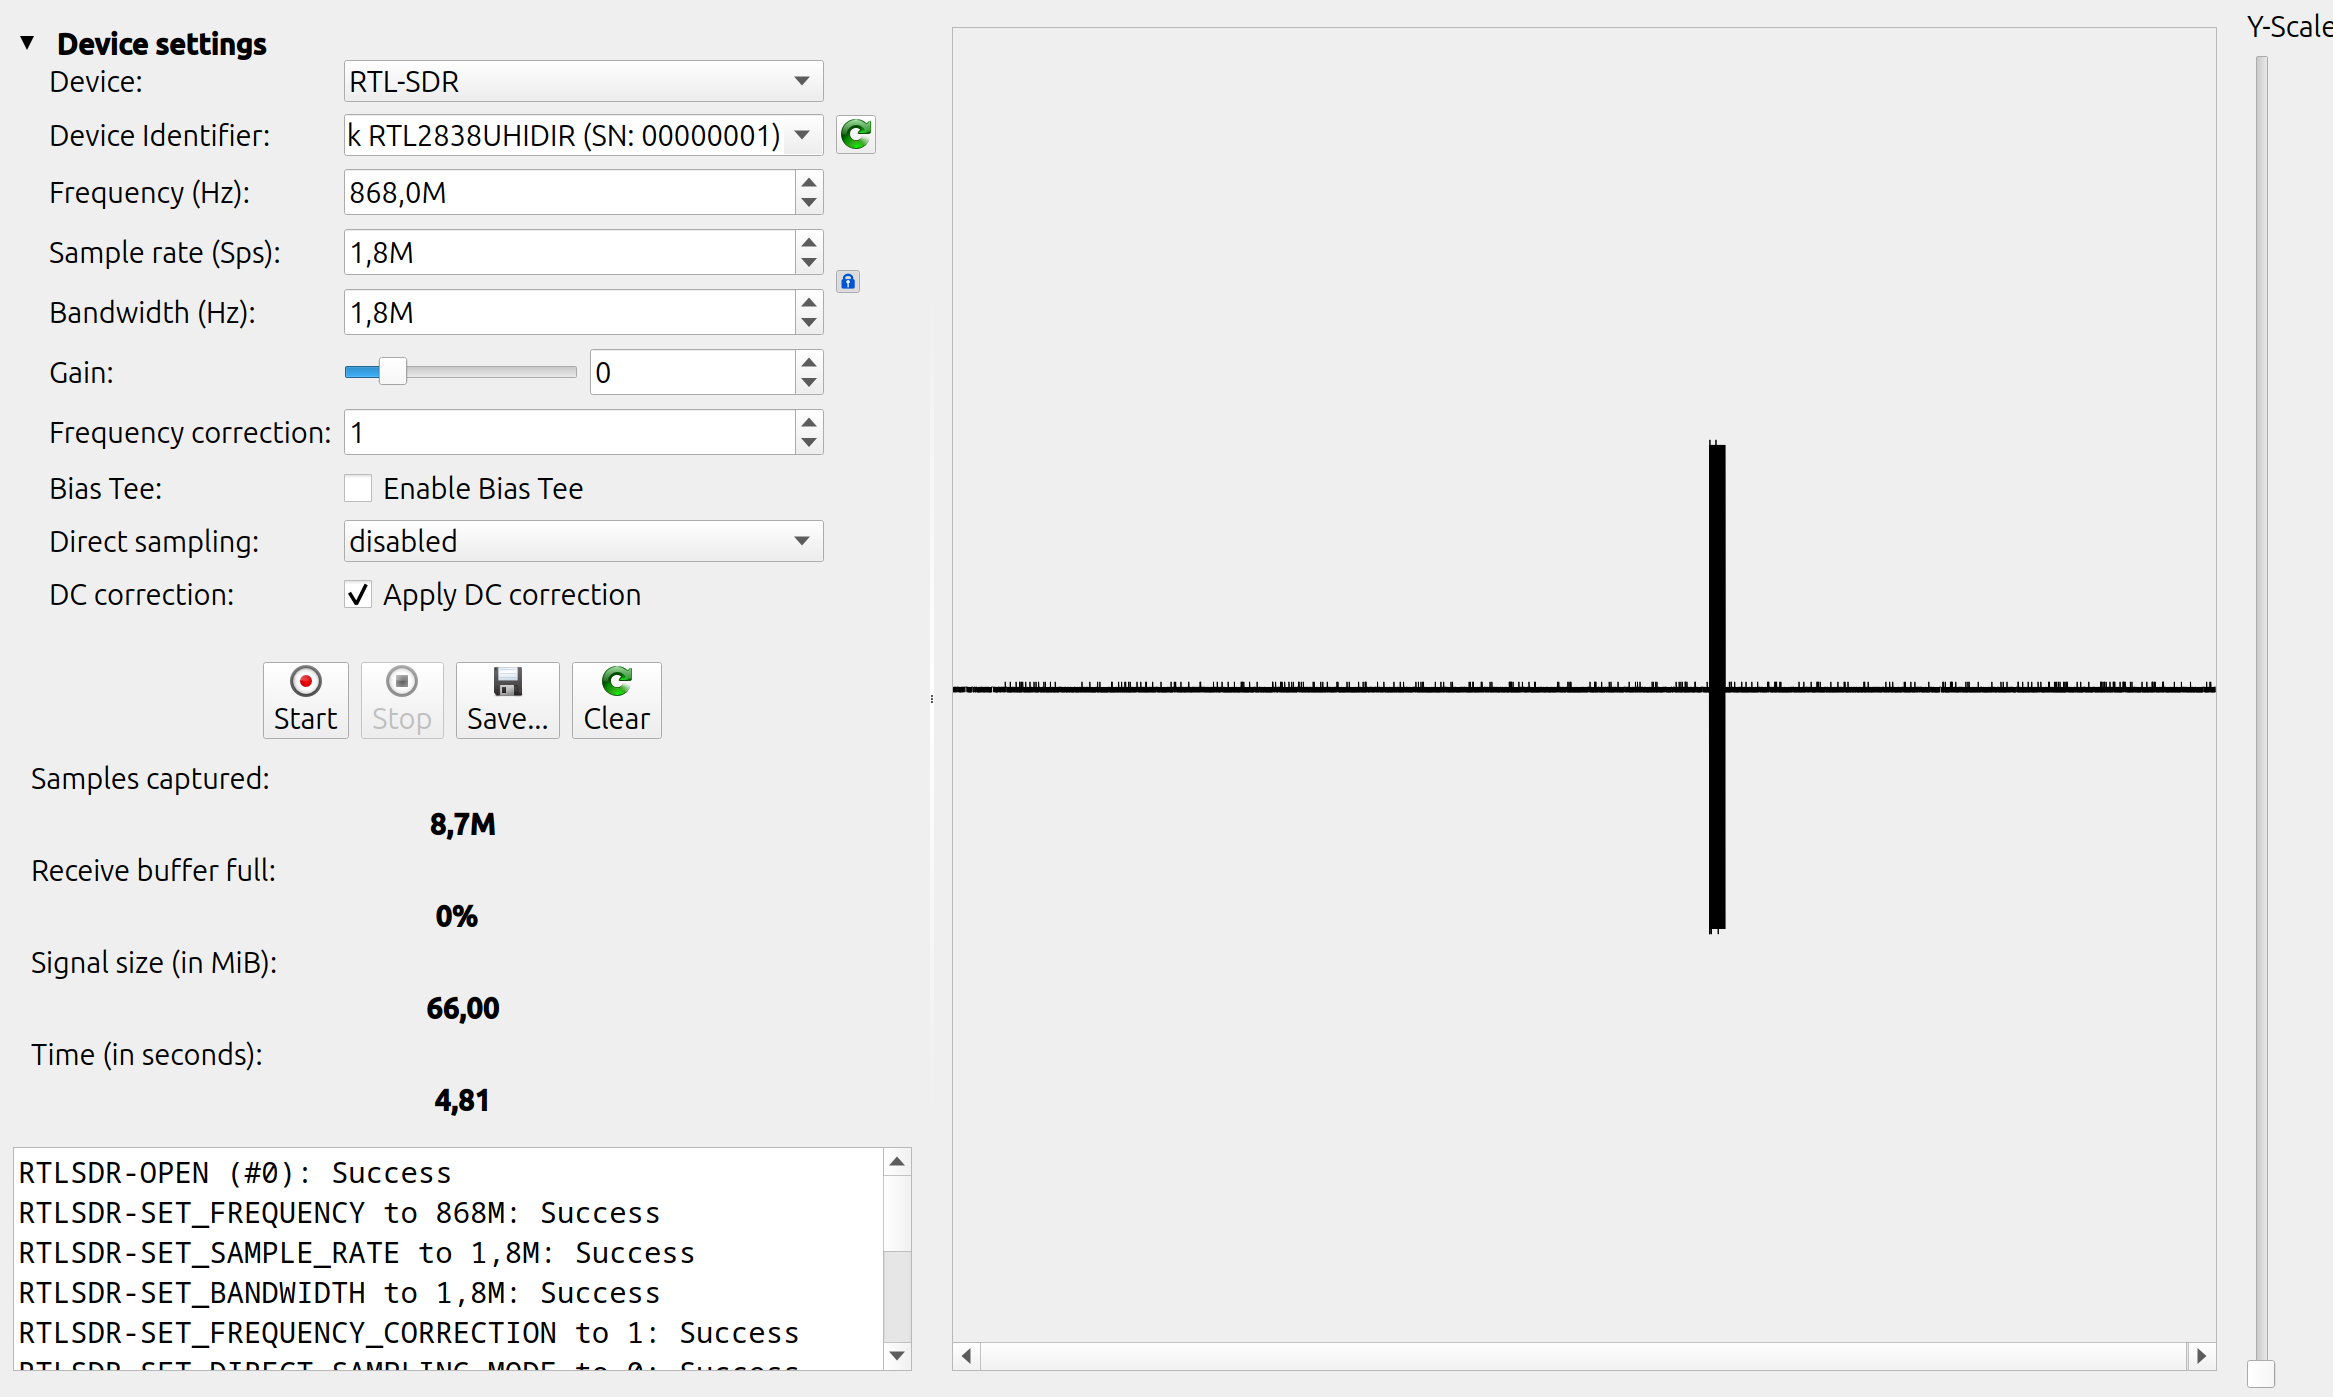
\includegraphics[scale=0.17]{images/urh2n.png}
\caption{Capture du signal}
\label{term303}
\end{figure}

\begin{figure}[h]
\centering

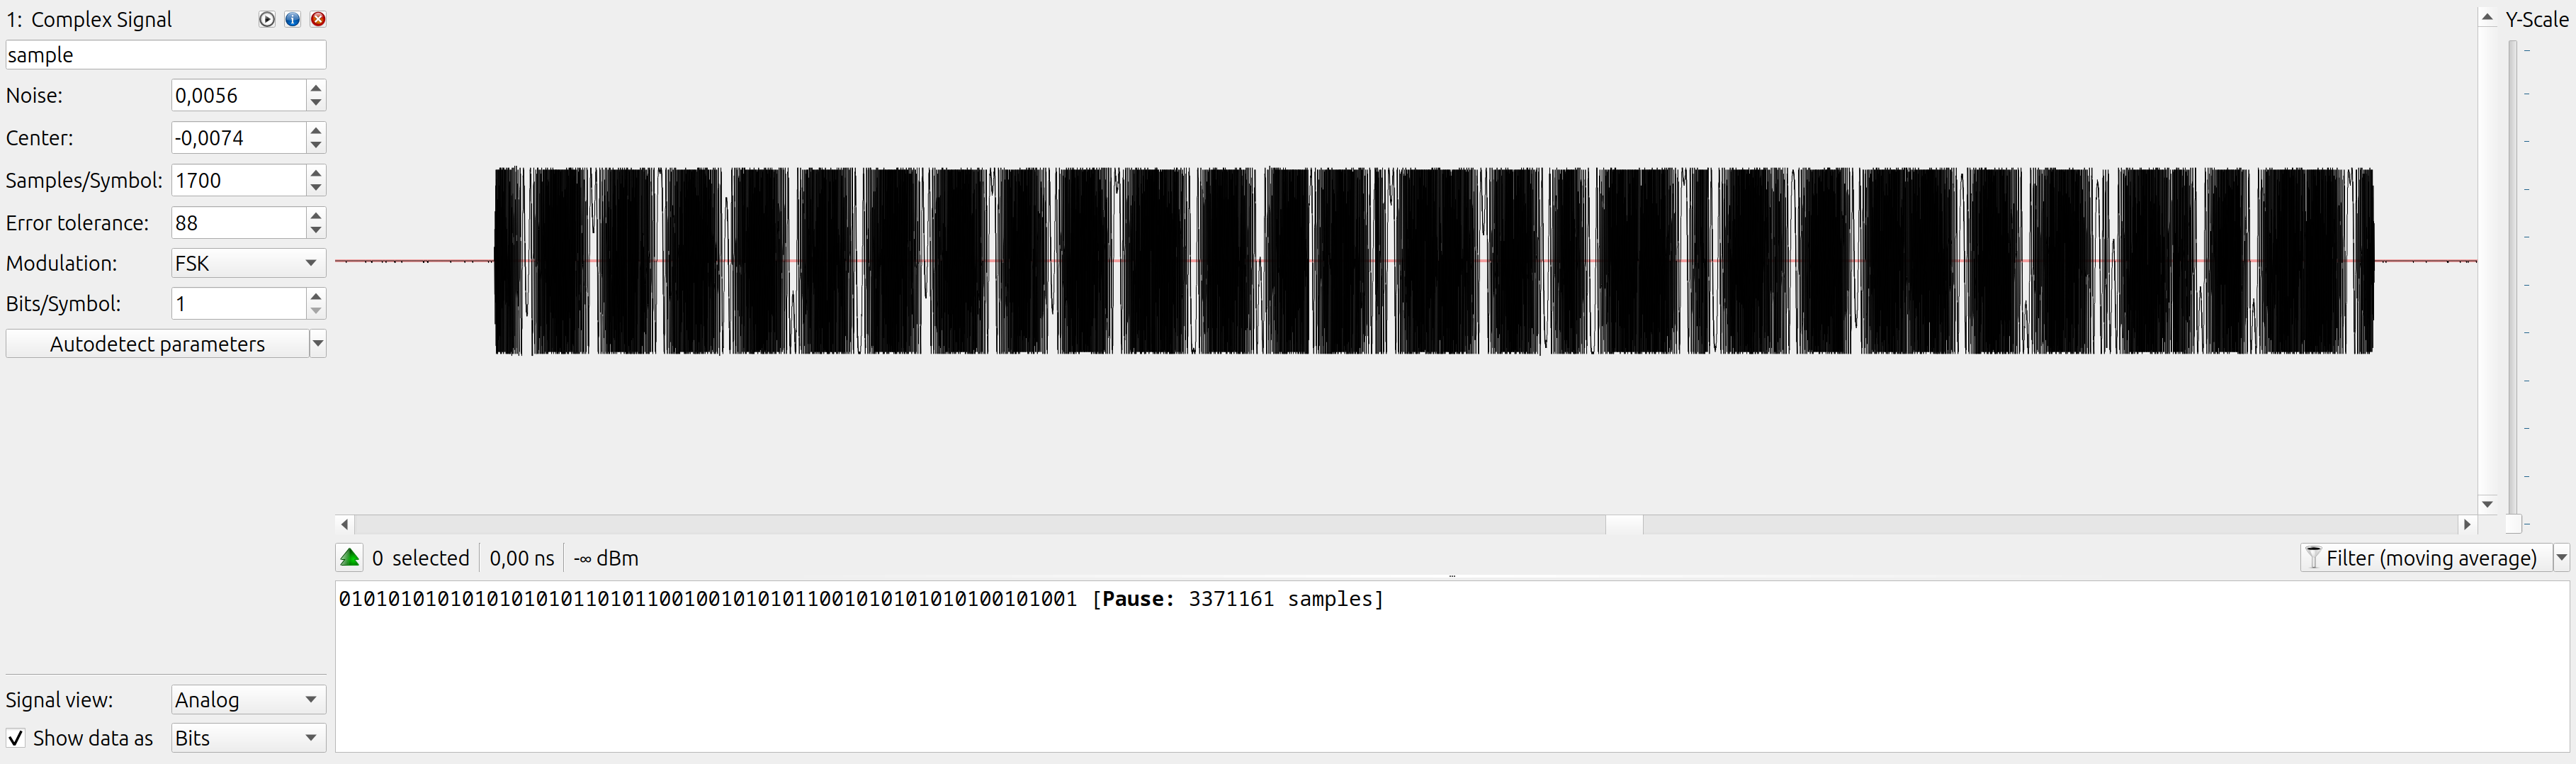
\includegraphics[scale=0.11]{images/urh3n.png}
\caption{Sauvegarde du signal}
\label{term304}
\end{figure}

A partir de la figure \ref{term304}, il est possible de couper une partie de l'enregistrement, notamment celle qui ne contient pas le signal. URH permet également d'afficher le signal sous forme de spectrogramme, la figure \ref{term306} montre le signal sous sa forme analogique et sous spectrogramme. On constate cependant que les deux affichages ne correspondent pas. En effet si on se fie au spectrogramme, la fréquence devrait augmenter durant le premier chirp, or quand on zoom sur le signal sur l'affichage analogique, celle ci diminue dans un premier temps. (voir figure \ref{term307}).

\newpage

\begin{figure}[h]
\centering

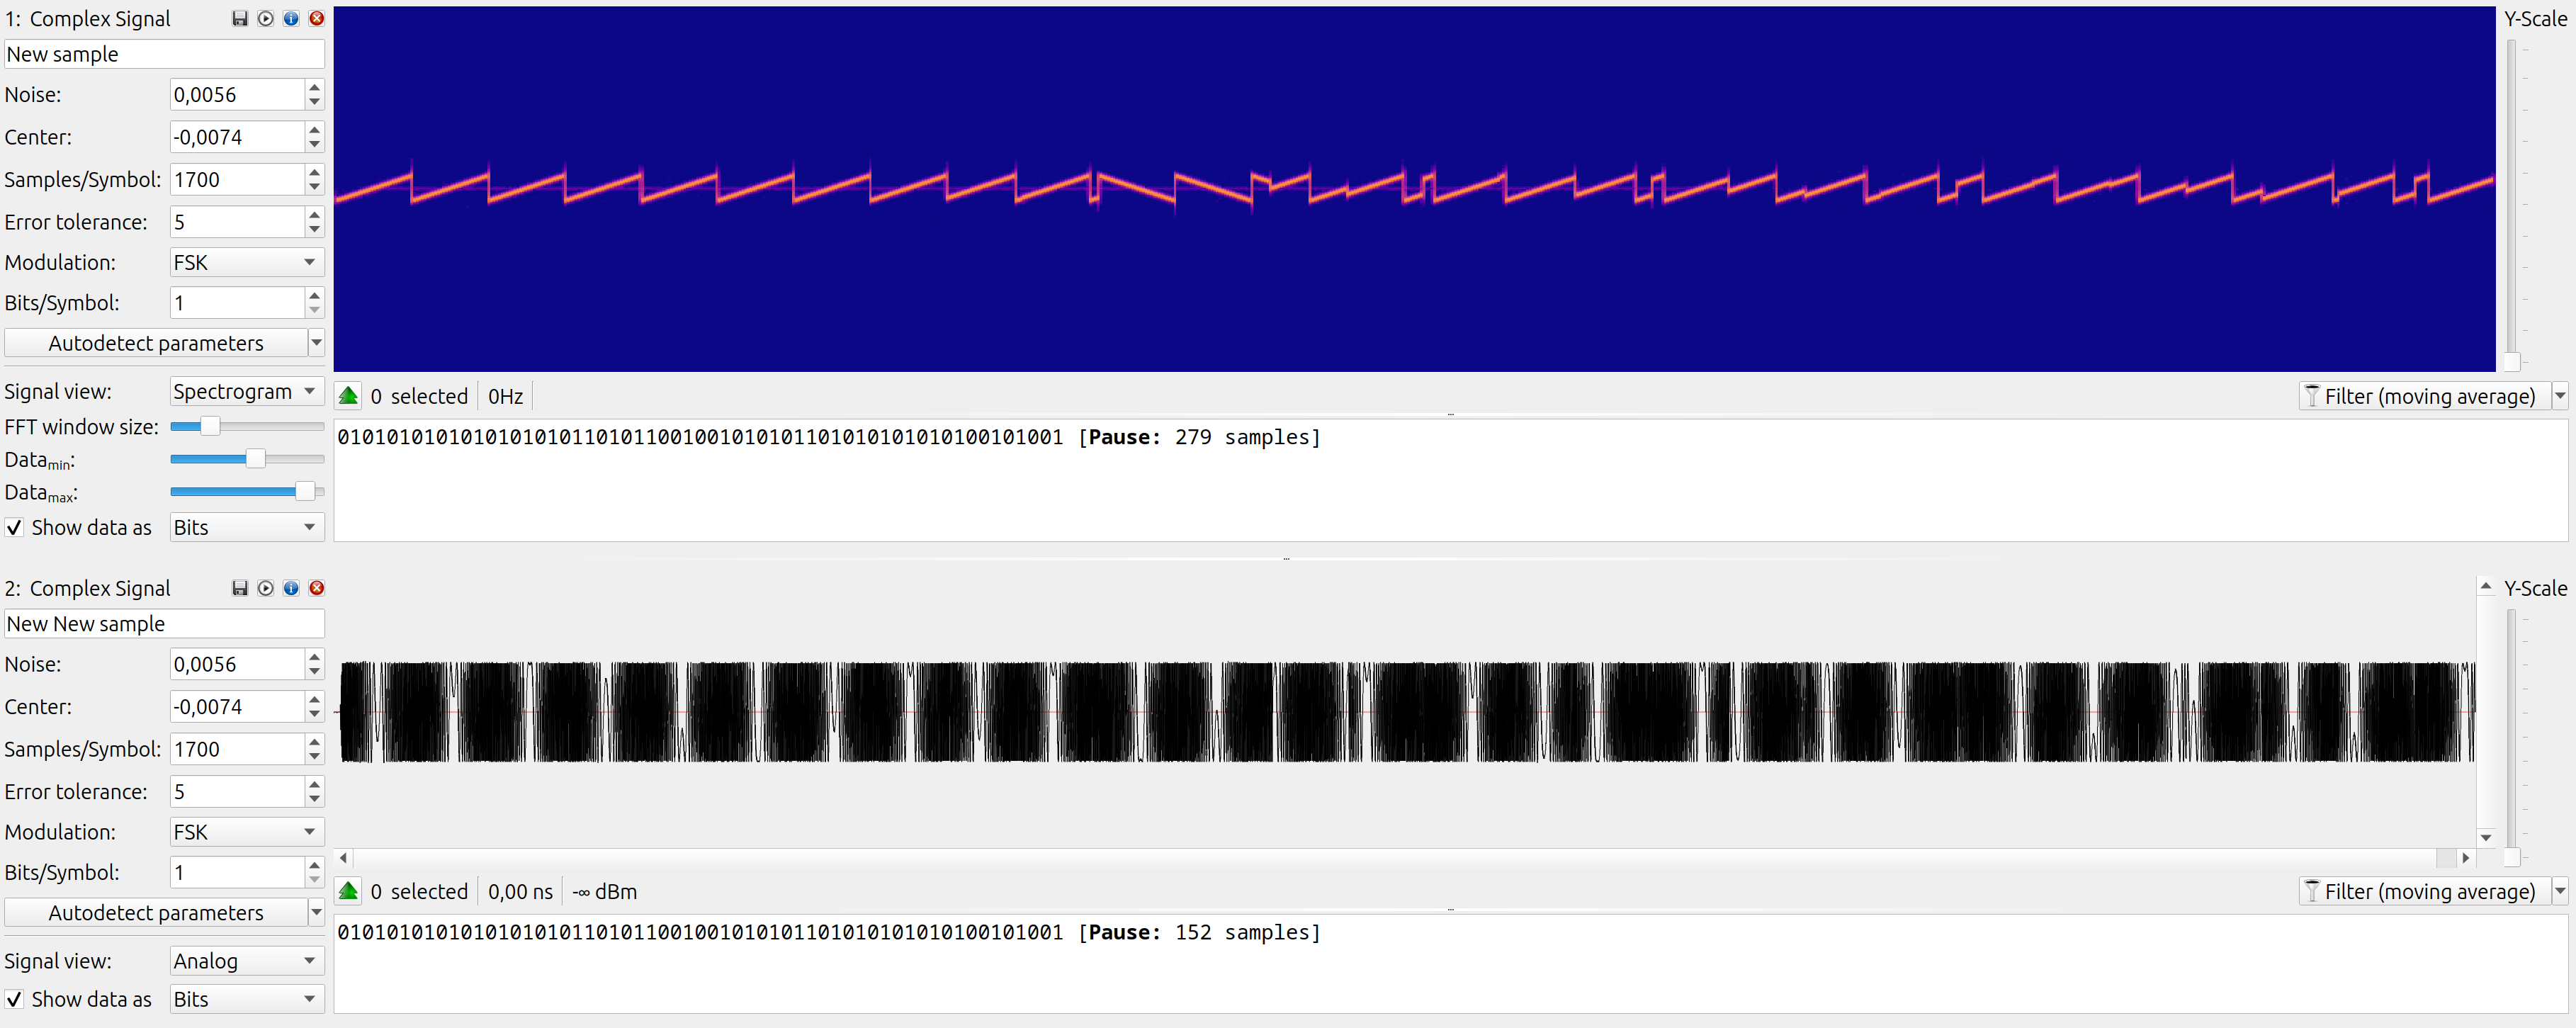
\includegraphics[scale=0.11]{images/urh4.png}
\caption{Signal LoRa sous forme spectrogramme et analogique}\label{term306}
\end{figure}

\begin{figure}[h]
\centering

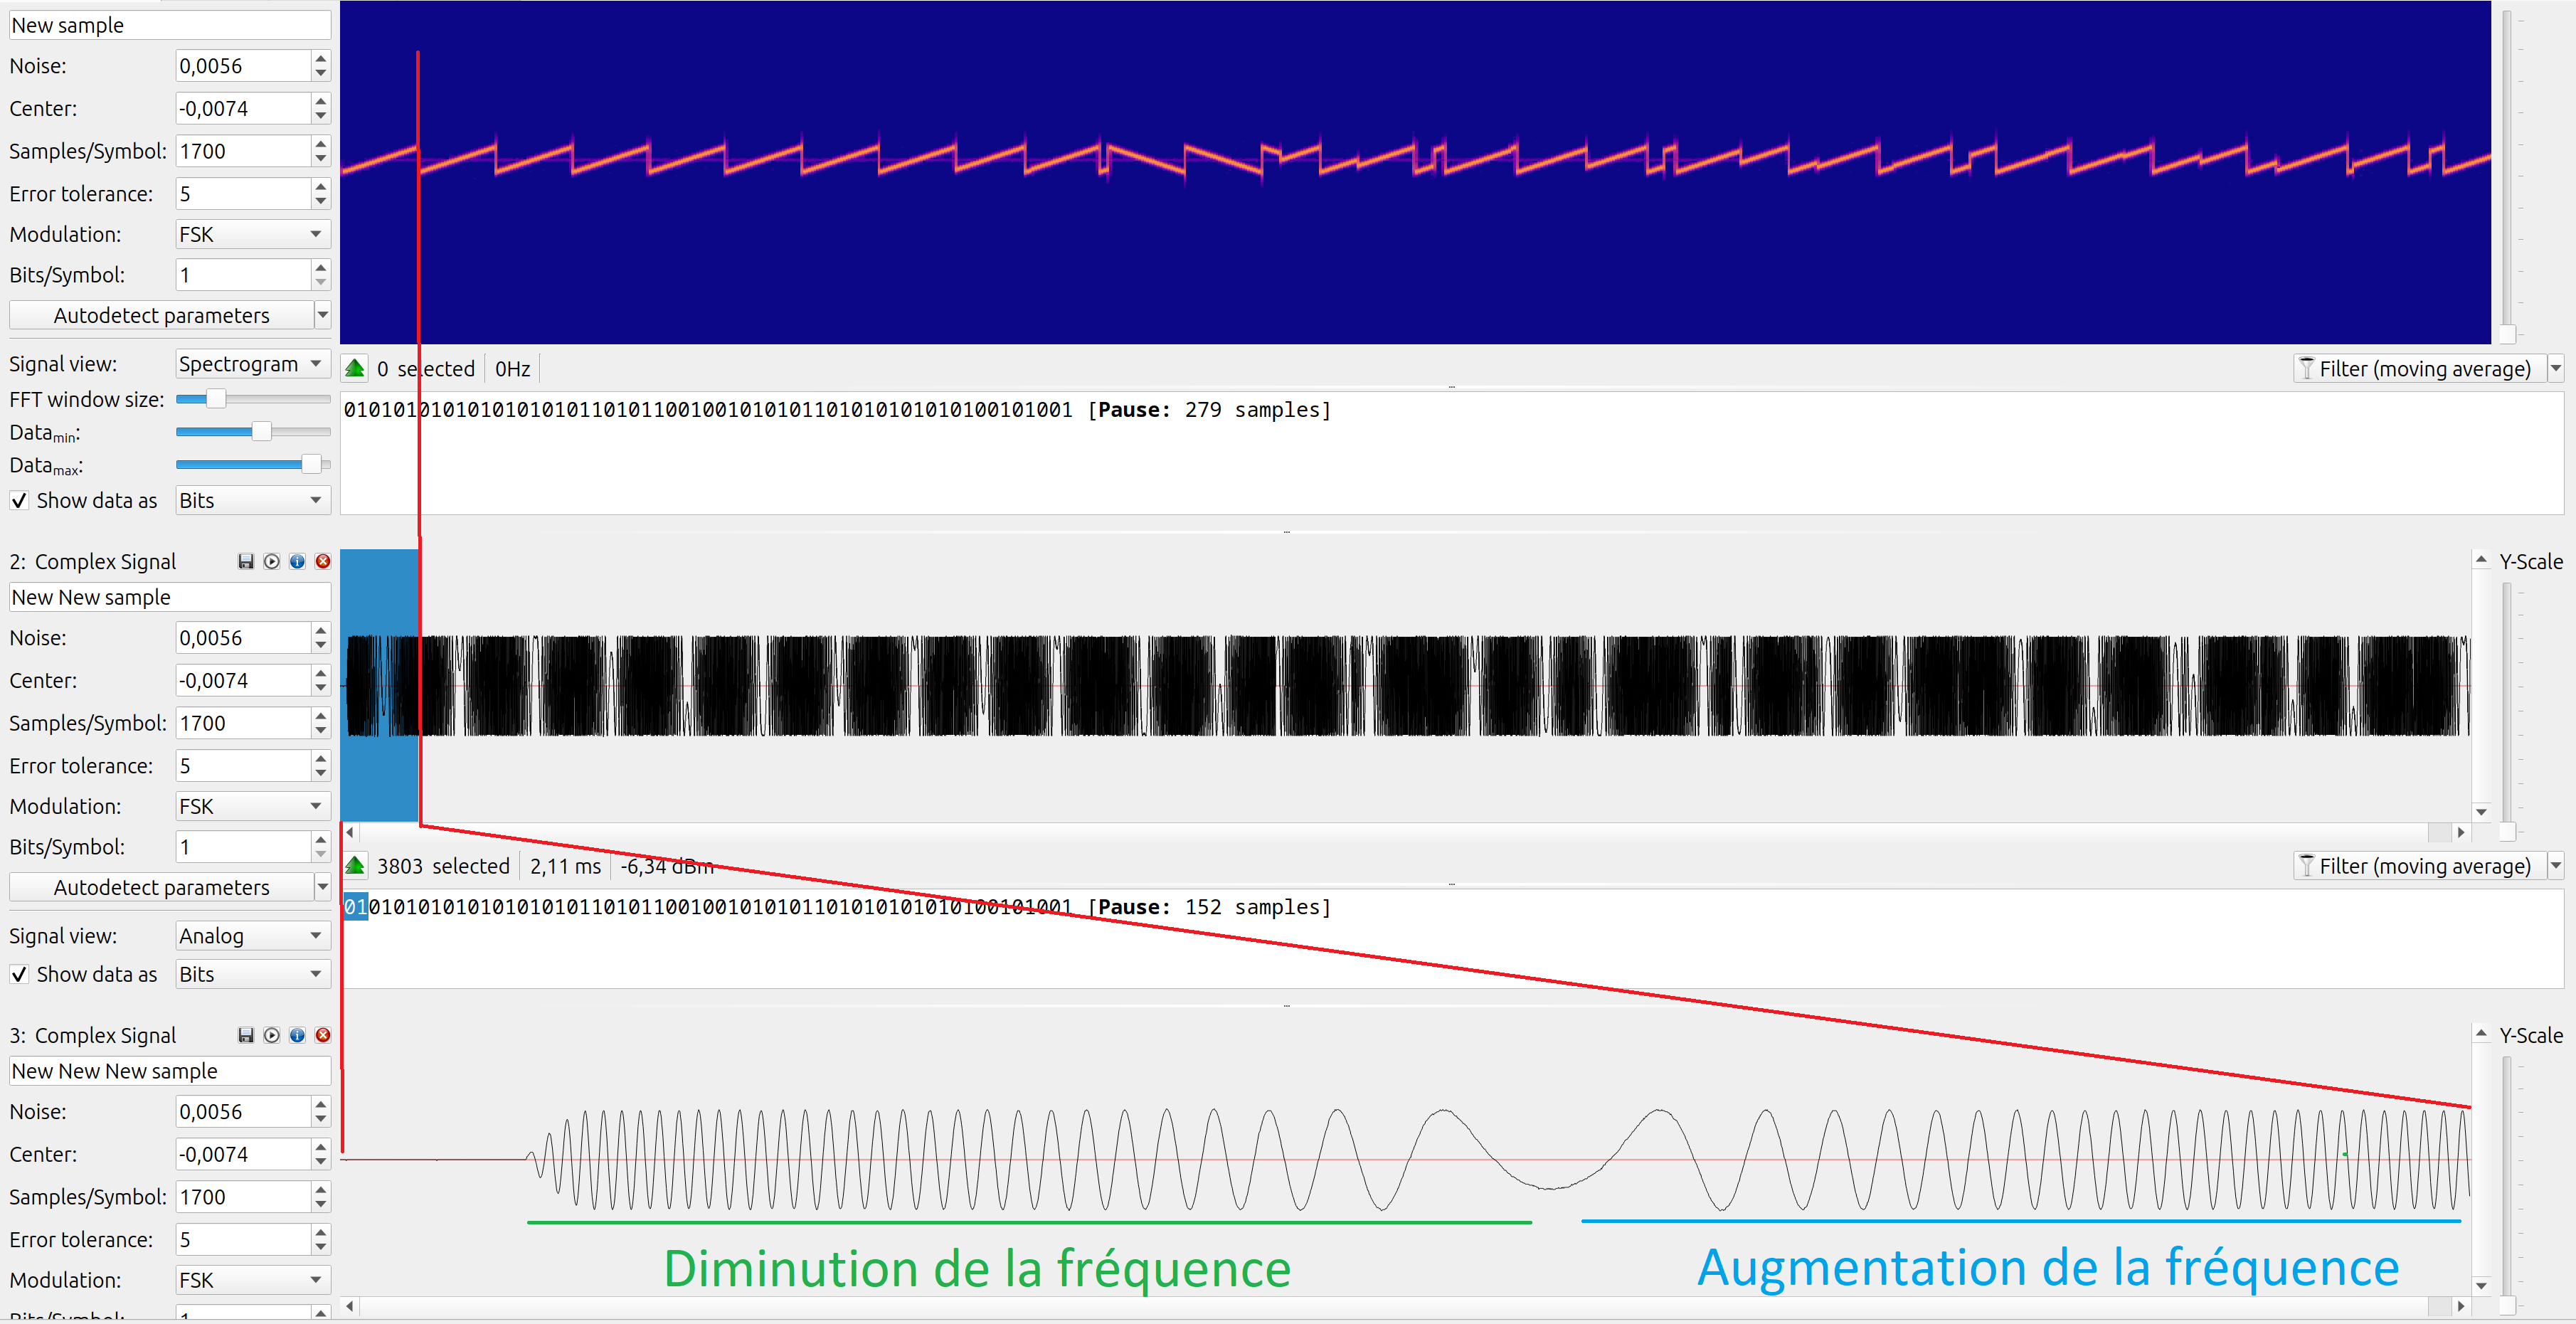
\includegraphics[scale=0.18]{images/urh5.png}
\caption{Zoom d'un upchirp du signal LoRa capturé}\label{term307}
\end{figure}

Ce phénomène est dû à une interprétation faussée par URH. La fréquence du récepteur choisie étant la même que celle de l'émetteur, URH va interpréter 868Mhz comme étant la fréquence centrale ayant pour valeur 0, ce qui signifie que pour un signal reçu à 868Mhz, la moitié des échantillons sont interprétés comme ayant une fréquence "négative". Autrement dit, URH affiche la position inverse des échantillons qu'il considère comme négatifs. Pour éviter cette erreur, il suffit de décaler la fréquence d'écoute proportionnellement à la moitié de la taille de la largeur de bande du signal émis. Dans ce cas, le signal émis à une largeur de bande de 125Khz, il aut ajuster la fréquence d'écoute :

\begin{align}
    F_{recepteur} = F_{emetteur} - \frac{BW}{2} soit: \\
    868Mhz - \frac{125KHz}{2} = 867,9375MHz
\end{align}

On observe également au début du premier chirp une période où l'amplitude est en train de s'ajuster. Ce phénomène appelé \textit{période transitoire (transcient part)} est un état instable durant lequel différentes propriétés du signal peuvent subir des changements. Sur la figure \ref{term307} cela survient au début de la réception, ce qui peut s'expliquer par le fait que le module d'émission change d'état au moment de débuter la transmission.

\vspace{0.1cm}

Selon la section \ref{packetlora}, la structure du paquet LoRa devrait contenir d'abord les symboles du préambule, soit 8 upchirps suivis de 4.25 chirps. La figure \ref{term308} montre le spectrogramme du signal complet, dont la partie fixe du préambule (les 8 upchirps par défaut) ont été mis en évidence sous forme analogique. Pouvoir identifier et récupérer le préambule du signal LoRa est crucial pour l'identification de l'appareil qui l'a émis.


\begin{figure}[h]
\centering

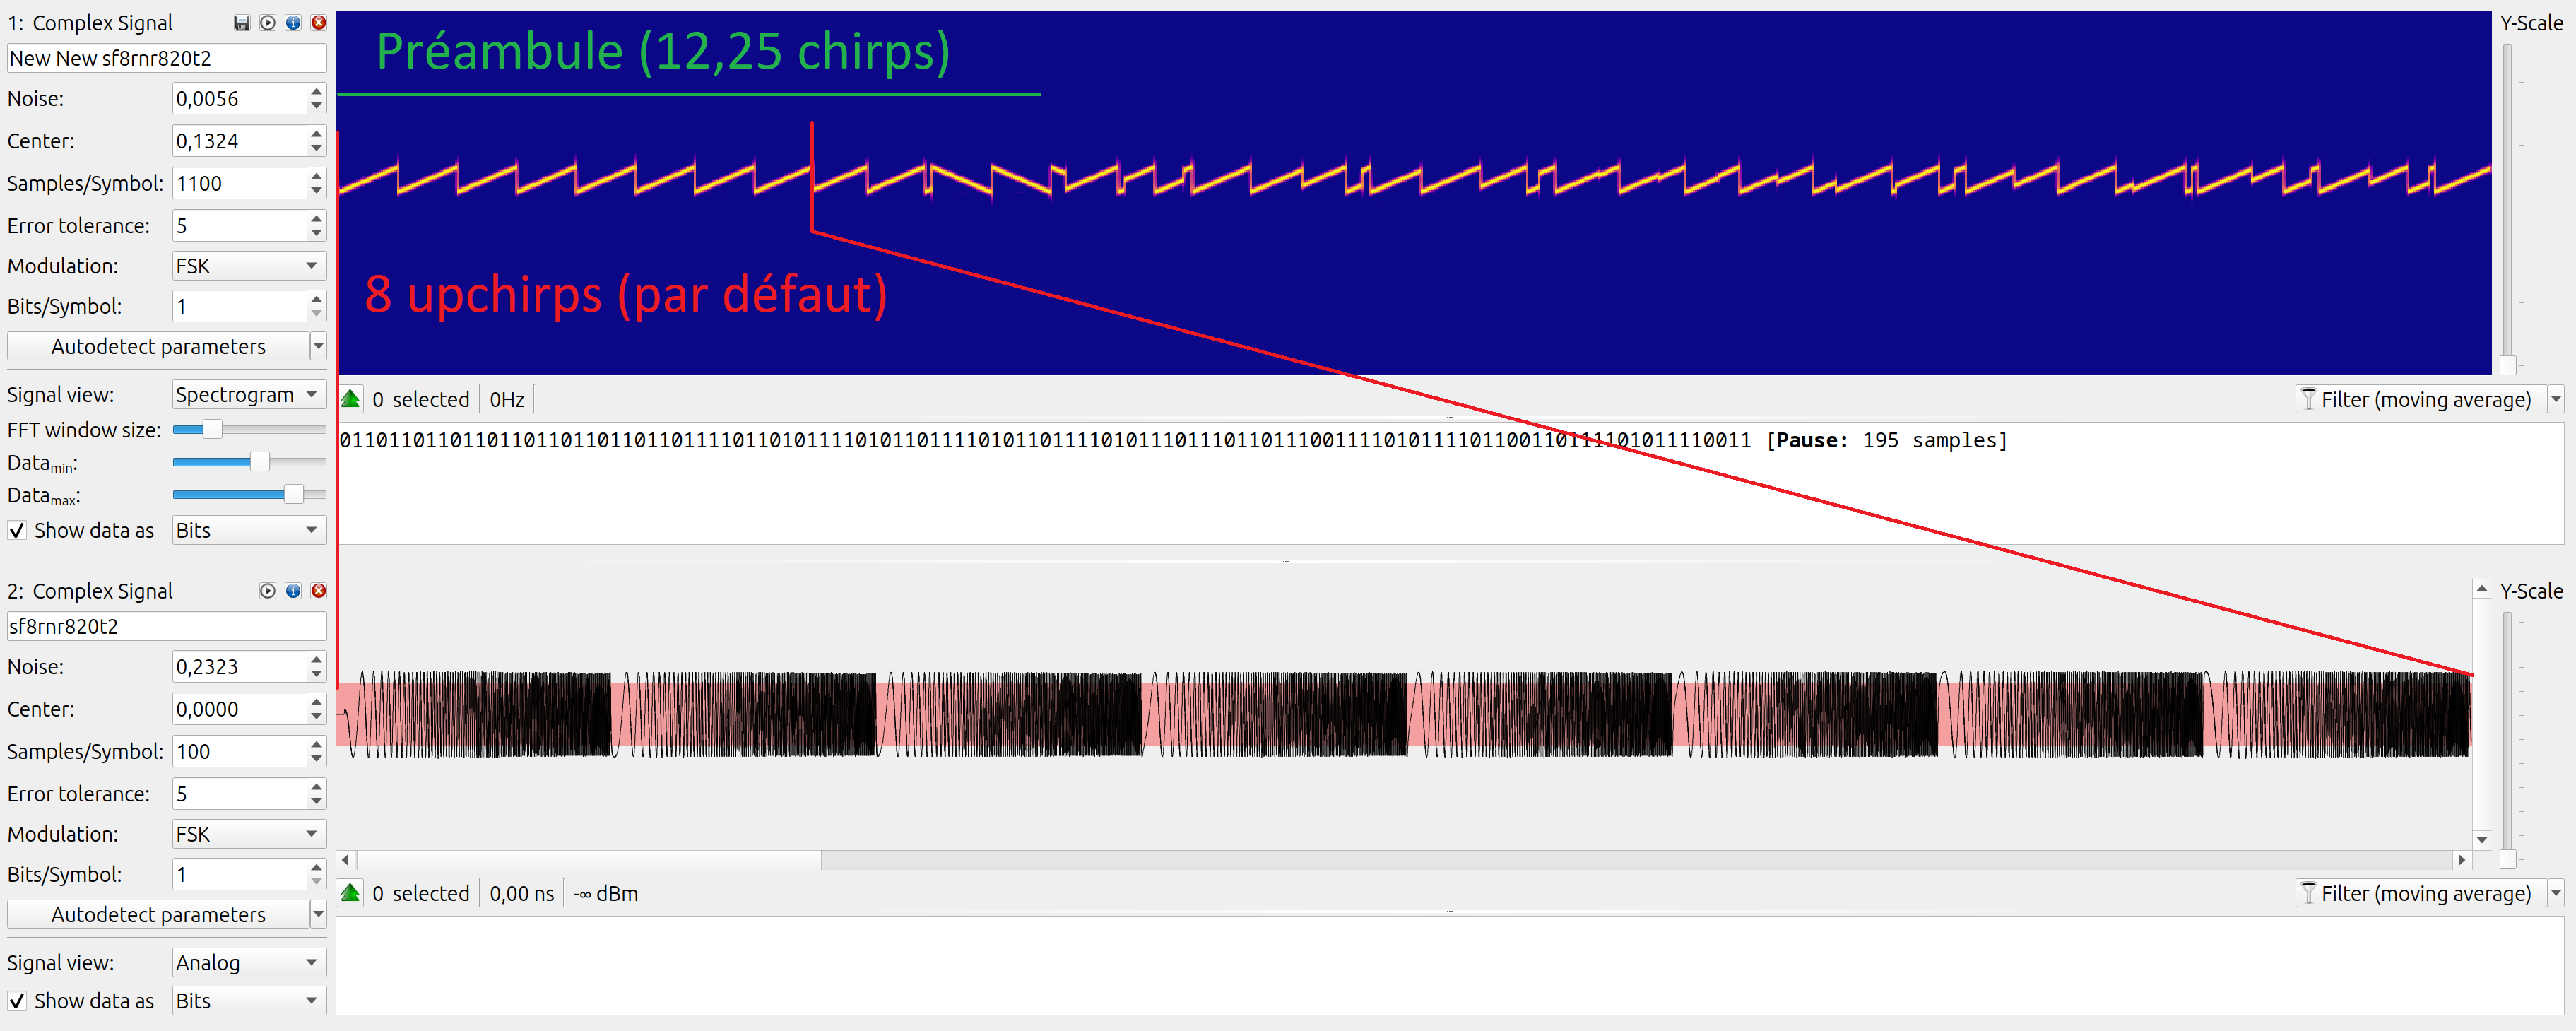
\includegraphics[scale=0.18]{images/urh6.png}
\caption{Identification du préambule LoRa}\label{term308}
\end{figure}

Cependant, l'utilisation d'intermédiaire comme URH ou GQRX n'est pas efficace pour traiter un grand nombre de signaux. La dernière étape avant de commencer l'identification des noeuds à partir des signaux est d'automatiser le processus complet de la capture du signal. Bien qu'URH et GQRX ne soit pas nécessaire pour réaliser l'indentification, leur utilisation a été d'une grande utilité. Par exemple pour l'apprentissage de la reconnaissance de signaux LoRa et de leur représentation, mais également pour l'observation de la partie transitoire d'un signal. Ils ont également permis de visualiser l'impact de paramètres comme le taux d'échantillonnage, le facteur d'étalement ou encore la largeur de bande d'un signal.

\subsection{Analyse avec python}

Une information importante que les deux logiciels de visualisation ont occultée, c'est la composition du signal. En effet, la visualisation analogique du signal avec URH montre une seule onde continue. Cependant il s'agit d'un signal complexe composé de deux ondes distinctes. Les échantillons du signal capturés par la SDR sont composés de deux composantes : la composante \textit{I (In phase}) et la composante \textit{Q (Quadrature)} (voir section \ref{mod}). URH combine les deux pour générer la vue analogique.

\vspace{0.1cm}

La librairie \textit{Matplotlib} de python permet d'afficher le contenu du signal capturé. La figure  \ref{term309} est un plot des échantillons dont la partie réelle (orange) et imaginaire (bleue) ont été séparées. Le signal a été capturé avec un taux d'échantil\-lonnage de 1.8MHz, malgré un TOA relativement court (quelques centièmes de secondes, le calcul du TOA est donné par l'équation \ref{toa}) la quantité d'échantillons capturés est très grande (plus de 130000 échantillons). Matplotlib permet également le zoom, la figure \ref{term310} fait un zoom sur les 4000 premiers échantillons. Les deux ondes apparaissent grâce au zoom.

\begin{figure}[h]
\centering

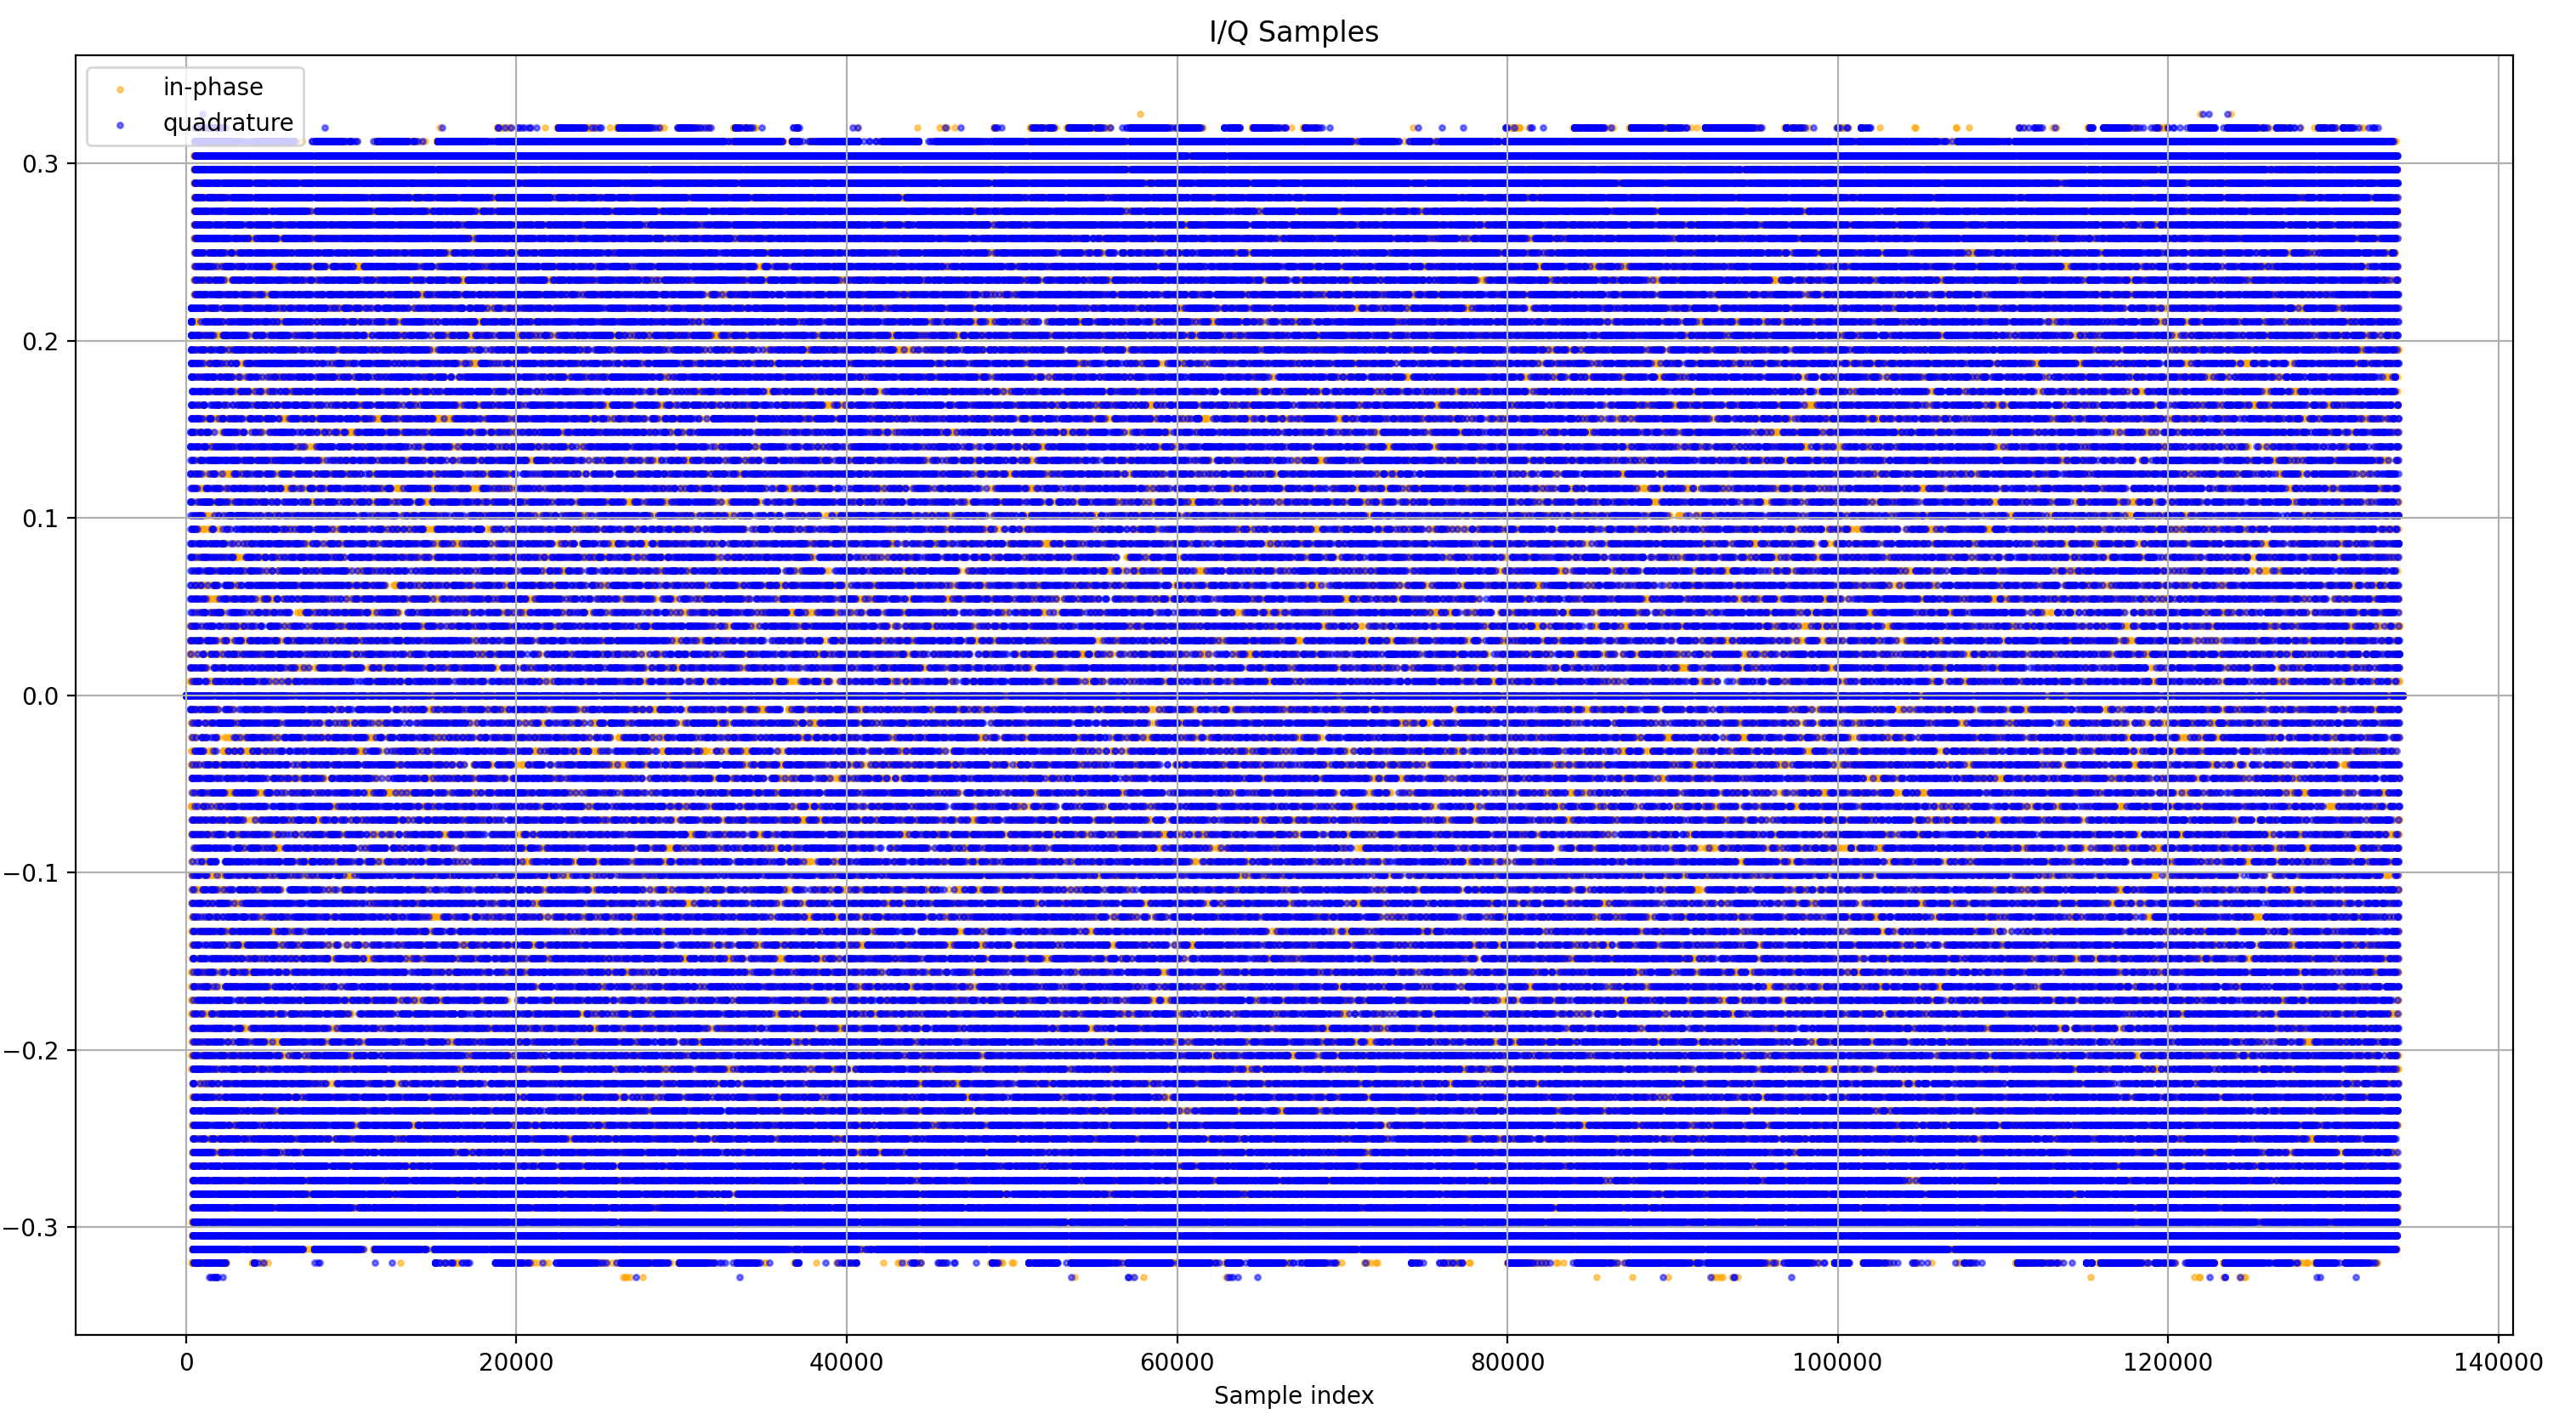
\includegraphics[scale=0.13]{images/iq1.png}
\caption{Plot des échantillons I/Q avec matplotlib}\label{term309}
\end{figure}



\newpage

\begin{figure}[h]
\centering

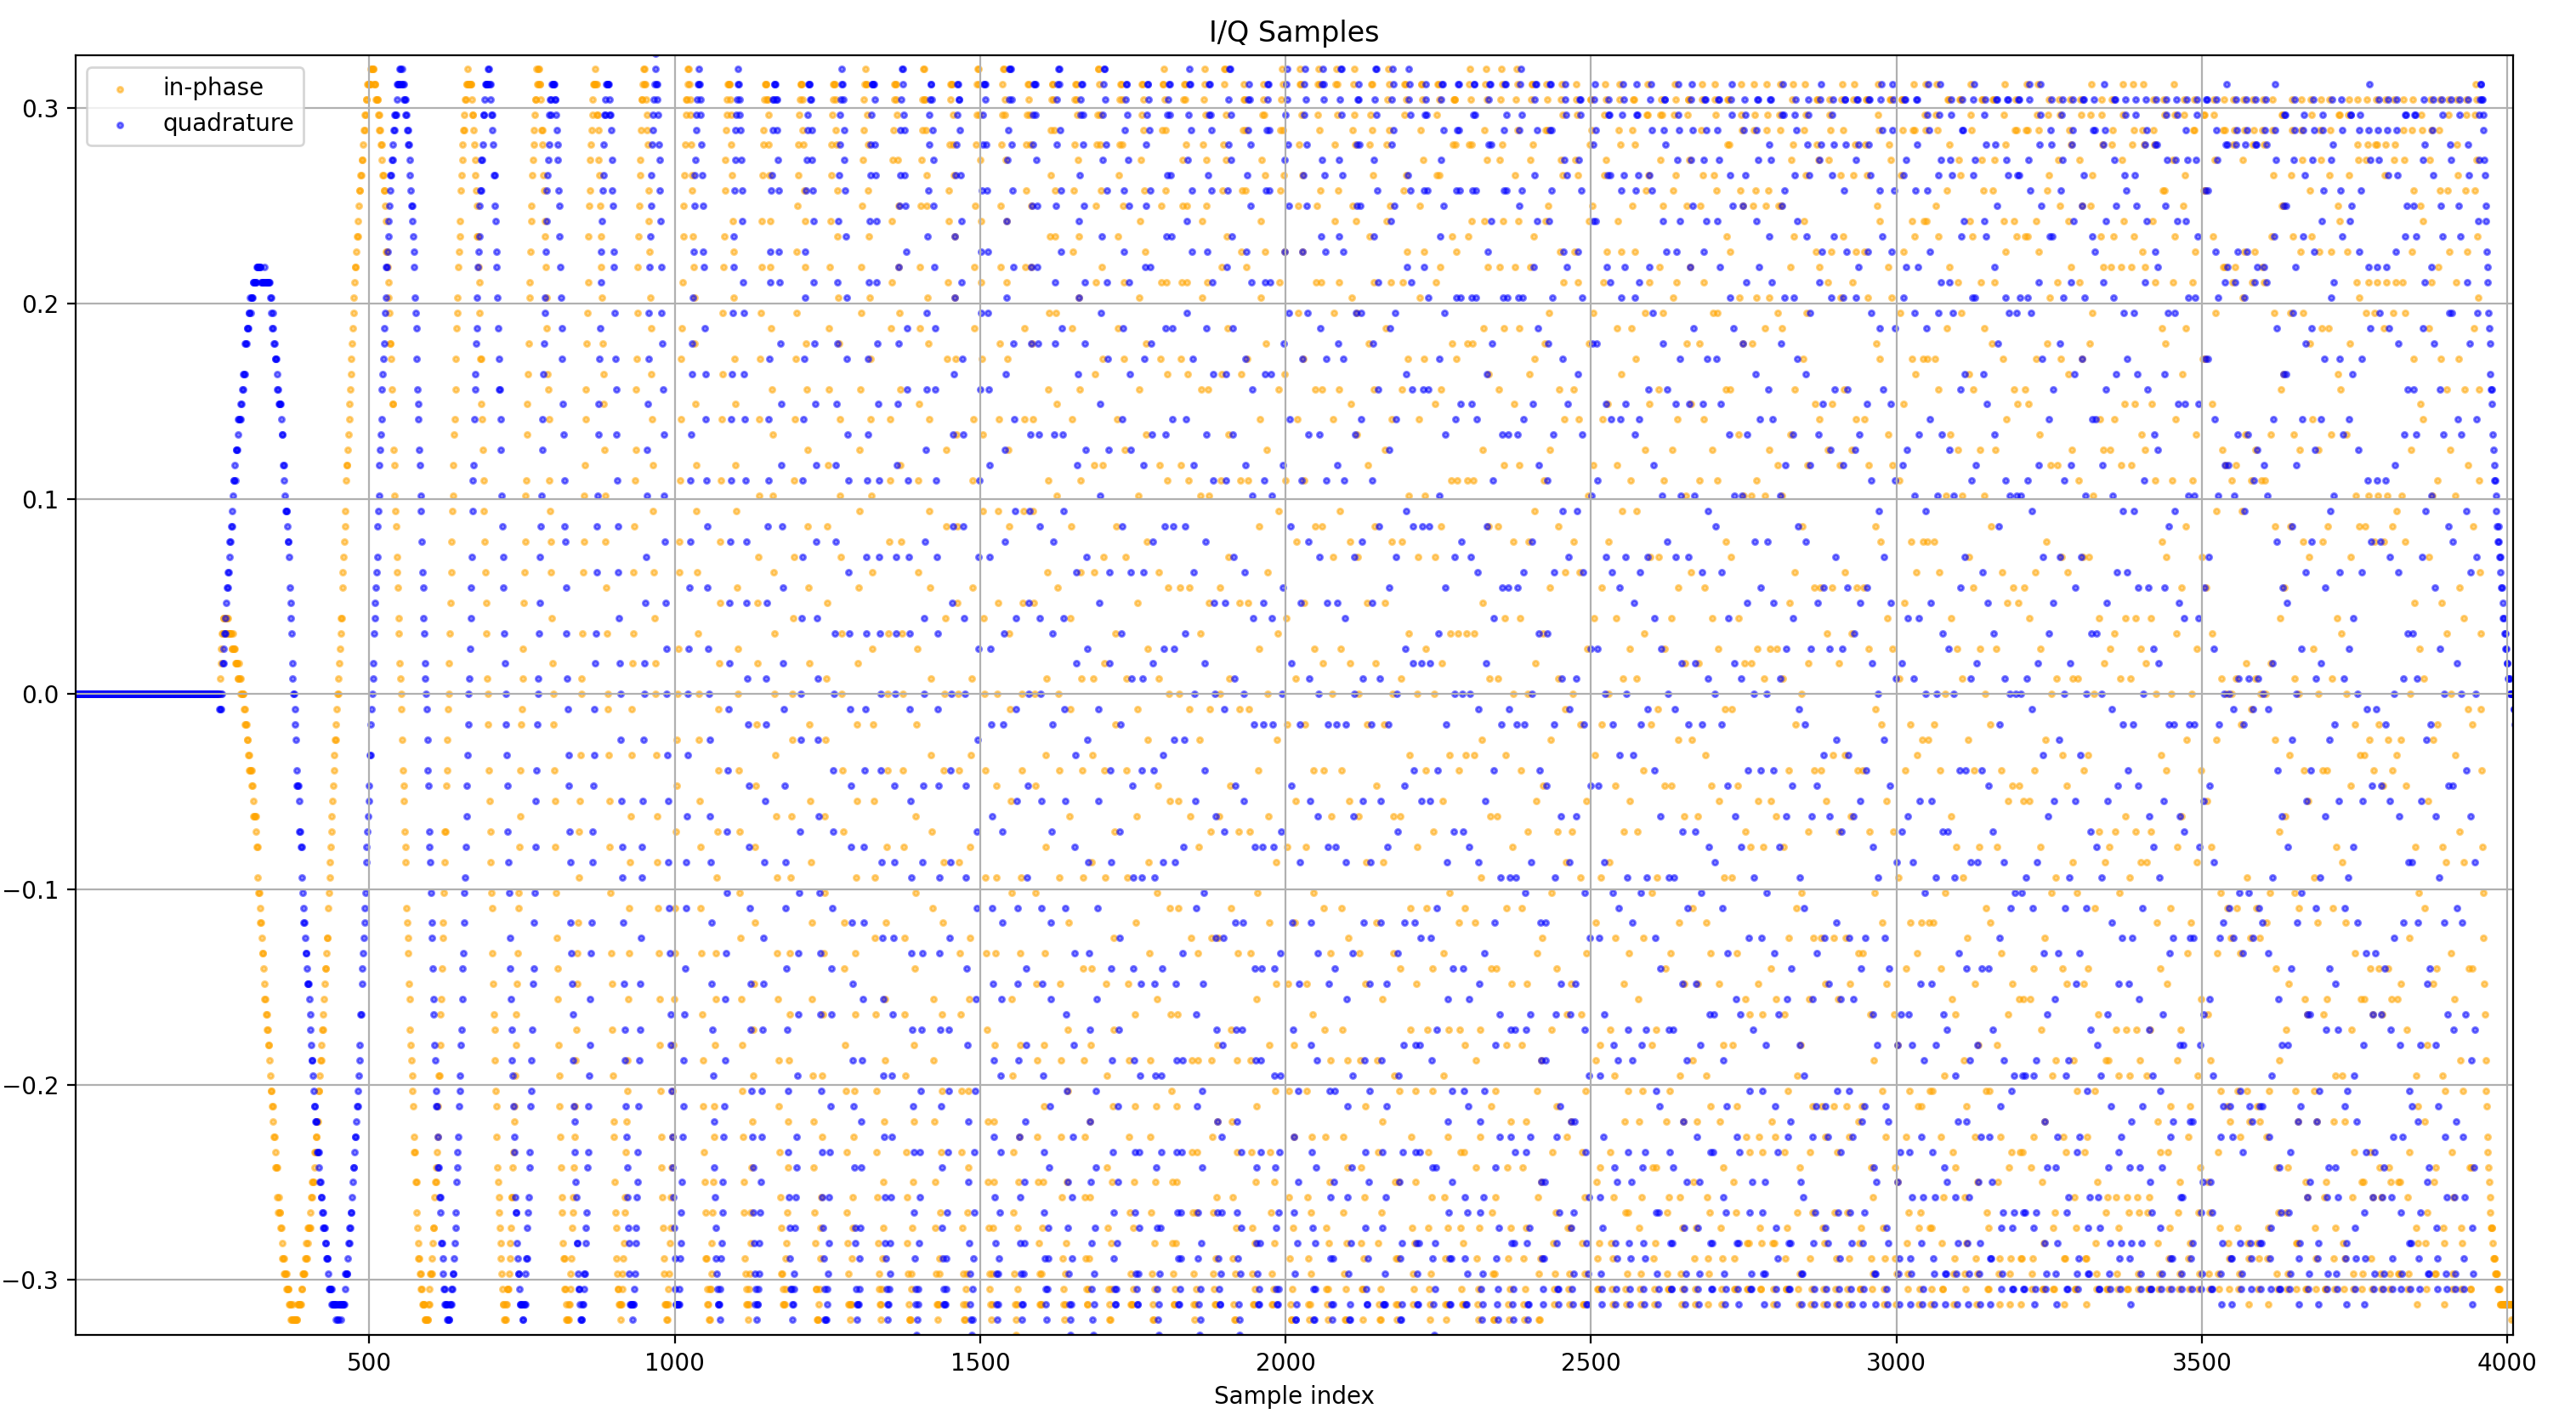
\includegraphics[scale=0.13]{images/iq2.png}
\caption{zoom sur les 4000 premiers échantillons I/Q}\label{term310}
\end{figure}

\subsection{Automatisation du signal et preprocessing}

Afin de pouvoir effectuer l'identification des appareils, il faut que l'environement de test soit identique pour chaque module, donc tous les paramètres d'émissions sont identiques. La même SDR est utilisé avec les mêmes paramètres de réception pour les mêmes raisons. Avec des paramètres d'émission et de réception fixes, il est possible d'automatiser le processus d'enregistrement d'échantillons LoRa.

La librairie PyRTLSDR permet de configurer la radio logicielle depuis un script python (voir annexe \ref{antenne}. La partie du signal que l'on cherche à conserver est le préambule (soit les 8 premiers chirps fixes ou les 12.25 premiers chirp). Si le taux d'échantillonnage ets fixe et que le préambule est toujours de la même taille, alors il est possible de calculer le nombre d'échantillons à capturer. 

Par exemple, la figure \ref{term311} indique qu'un préambule complet (12.25 chirp) contient environ 49000 échantillons. Sachant que le taux d'échantillonnage est de 2MHz pour cette exemple, alors le TOA du préambule vaut :

\begin{align}\label{toa}
    Time On Air (TOA) = \frac{N_{samples}}{sample rate} = 0.0245
\end{align}

\clearpage

\begin{figure}[h]
\centering

\includegraphics[scale=0.14]{images/iq3.png}
\caption{Préambule LoRa (sampel rate = 2MHz)}\label{term311}
\end{figure}

Maintenant que la durée de l'enregistrement est calculée, il reste à fixer le moment à partir duquel l'enregistrement commence. La méthode la plus facile est d'implémenter un threshold qui détermine si un signal est reçu durant l'écoute. Voici en résumé comment toute l'opération se déroule :

\begin{itemize}
\item Les paramètres de l'émetteur sont configurés. 
\item Dès que l'émetteur est prêt à envoyer un signal, le récepteur commence à écouter.
\item le récepteur informe l'émetteur que il est en écoute, l'émetteur envoie un signal.
\item Grâce au threshold, le récepteur commence à enregistrer le TOA du signal dès que le threshold est franchi. L'émetteur est en attente pendant que le signal est enregistré dans un fichier.
\item Le récepteur se remet sur écoute et informe l'émetteur qu'il peut envoyer un nouveau signal.
\end{itemize}

Finalement, il reste une dernière étape avant de pouvoir commencer l'identification des modules. Bien que les prises d'échantillons soient en intérieur avec une faible distance entre l'émetteur et le recepteur (voir figure \ref{term312}), les signaux sont parfois fortement atténués. Il faut donc normaliser les données pour contrer les différences d'amplitude. Les données sont normalisées en utilisant \textit{Root means square (RMS)}. La valeur du RMS pour un set $x$ de $n$ données ${x_1,x_2,...,x_n}$ vaut la racine carrée de la moyenne arithmétique des carrés des valeurs soit :

\begin{align}
    x_{RMS} = \sqrt{\frac{1}{n}(x_1^2 + x_2^2 + ... + x_n^2}
\end{align}

L'implémentation de l'automatisation et de la normalisation est disponible en annexe \ref{codeauto}. L'application de RMS a lieu une fois que les données ont été sauvegardées en fichier. Pour chaque répertoire contenant différents signaux capturés, RMS est appliqué individuellement sur chacun des fichiers.

\begin{figure}[h]
\centering

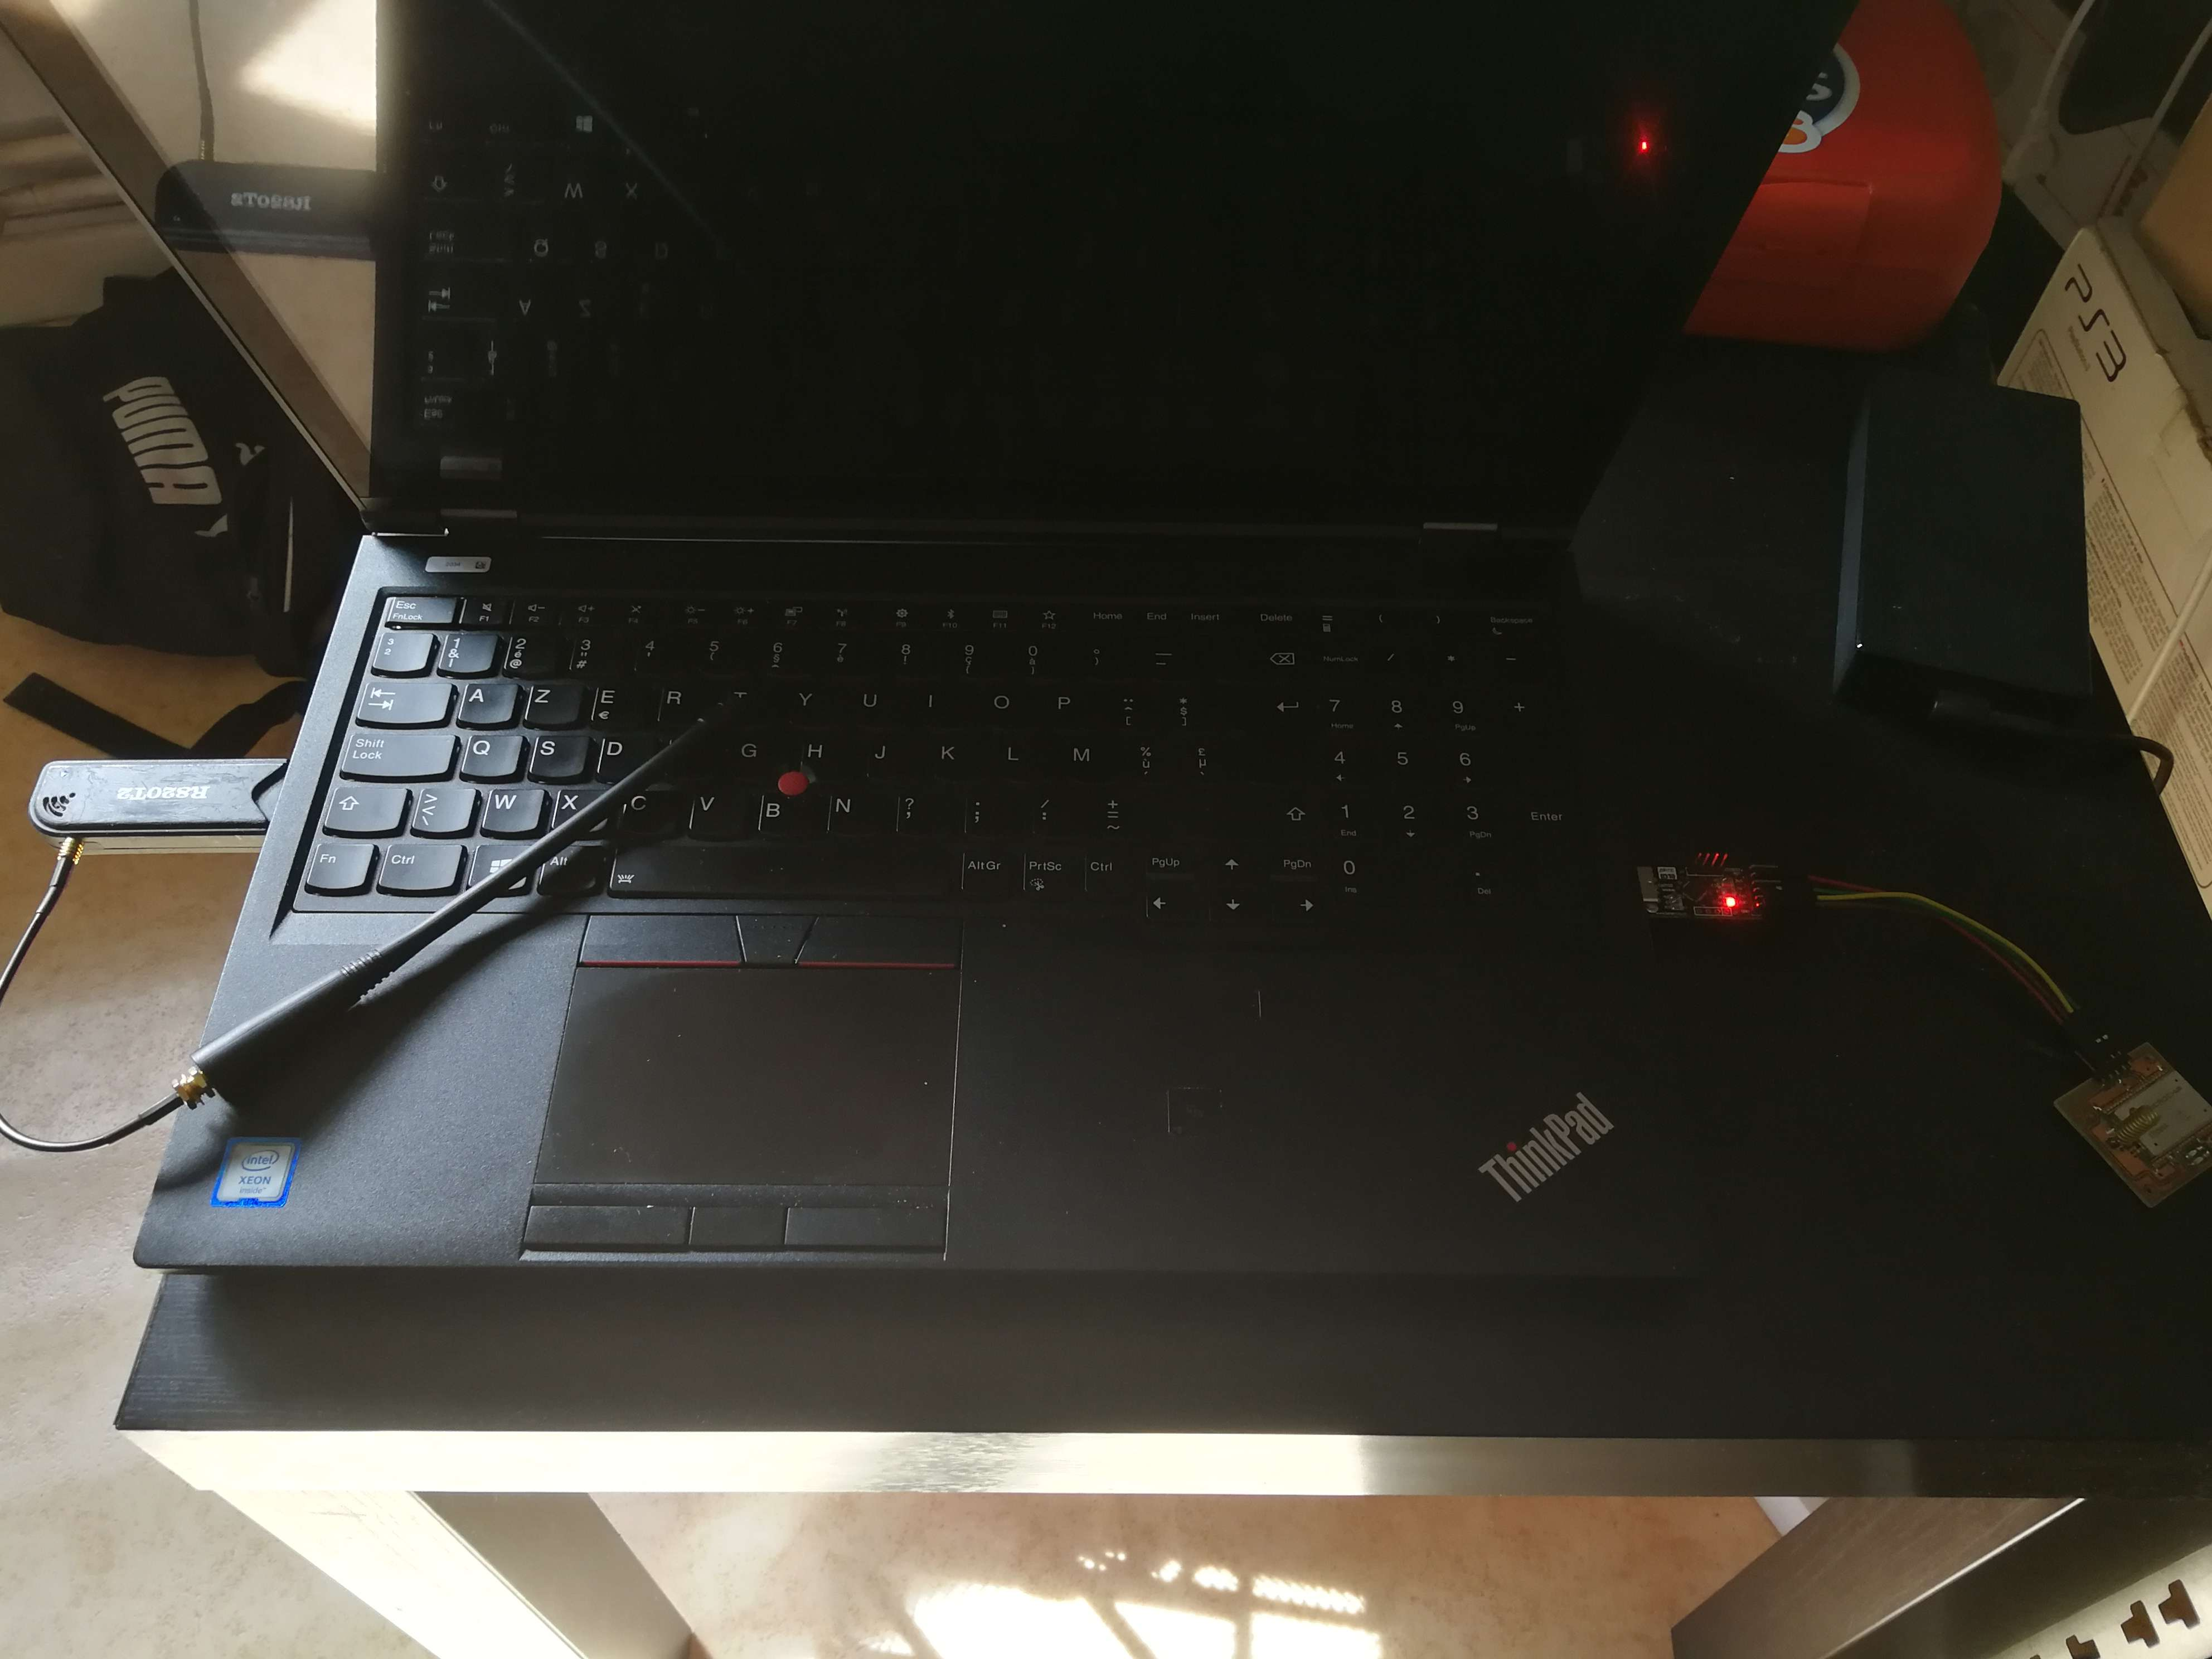
\includegraphics[scale=0.08]{images/conf1.png}
\caption{Configuration en intérieur}\label{term312}
\end{figure}